\documentclass[acmsmall,screen,review]{acmart}
\settopmatter{printfolios=true,printccs=false,printacmref=false}
\renewcommand\footnotetextcopyrightpermission[1]{}

\usepackage{booktabs}
\usepackage{bbm}
\usepackage{ebproof}
\usepackage{minted}
\usepackage{tikz-cd}
\usepackage{subcaption}

% Parameters {{{
%% Rights management information.  This information is sent to you
%% when you complete the rights form.  These commands have SAMPLE
%% values in them; it is your responsibility as an author to replace
%% the commands and values with those provided to you when you
%% complete the rights form.
%% \setcopyright{none}
\setcopyright{acmcopyright}
\copyrightyear{2018}
\acmYear{2018}
\acmDOI{XXXXXXX.XXXXXXX}
\acmConference[]{}{}{}
\acmPrice{15.00}
\acmISBN{978-1-4503-XXXX-X/18/06}

\bibliographystyle{ACM-Reference-Format}
%\citestyle{acmauthoryear}
%}}}

\hyphenation{Comp-Cert}
\hyphenation{Comp-CertX}
\hyphenation{Comp-CertO}
\hyphenation{Comp-CertM}
\hyphenation{Certi-KOS}


% Notations {{{
\newcommand{\kw}[1]{\ensuremath{ \mathsf{#1} }}
\newcommand{\ifr}[1]{\mathrel{[{#1}]}}
\newcommand{\que}{\circ}
\newcommand{\ans}{\bullet}
\newcommand{\vref}{\le_\kw{v}}
\newcommand{\mext}{\le_\kw{m}}
\newcommand{\refby}{\preceq}
\newcommand{\scref}{\sqsupseteq}
\newcommand{\screfd}{\sqsubseteq}
\newcommand{\unitset}{\mathds{1}}
\renewcommand{\preceq}{\le}
\newcommand{\intl}[1]{\underline{#1}}
%\newcommand{\caller}[1]{{\rtimes}#1}
%\newcommand{\callee}[1]{{\ltimes}#1}
\newcommand{\caller}[1]{\langle #1 ]}
\newcommand{\callee}[1]{[ #1 \rangle}
\newcommand{\lensarrow}{\leftrightarrows}
\newcommand{\lensle}{\preccurlyeq}
%}}}

% Names of things {{{
\newcommand{\ClightP}{\ensuremath{ \mathsf{ClightP} }}
\newcommand{\Clight}{\ensuremath{ \mathsf{Clight} }}
%}}}

% Helpful shortcuts {{{
\newcommand{\draftfig}[2]{%
  \vcenter{\hbox{%
    \includegraphics[scale=#1]{draftfig/#2}%
  }}%
}
%}}}

% Custom symbols {{{
\makeatletter
\providecommand*{\cupdot}{%
  \mathbin{%
    \mathpalette\@cupdot{}%
  }%
}
\newcommand*{\@cupdot}[2]{%
  \ooalign{%
    $\m@th#1\cup$\cr
    \hidewidth$\m@th#1\cdot$\hidewidth
  }%
}
\makeatother
%}}}

%\title{Compositional Compiler Correctness with Encapsulated State}
\title{A Framework for Compositional Verification with
  Data Abstraction, Encapsulated State and Certified Compilation}

\begin{document}
\newtheorem{remark}[theorem]{Remark}

\begin{abstract} %{{{
Formal verification is the gold standard
for building reliable computer systems.
\emph{Certified} systems in particular
come with a formal specification,
and with a proof of correctness
which can easily be checked by a third party~%
\cite{shao10}.
Unfortunately, verifying large-scale, heterogeneous systems
remains out of reach of current techniques.
Addressing this challenge
will require the use of compositional methods,
making it easier to construct certified systems
from off-the-shelf certified components~\cite{deepspec}.

In principle,
compositional semantics
could play a key role in enabling this.
In practice, simpler operational models
have proven more amenable
to carrying out actual verification projects,
and few compositional semantic models
support the combination of features
required for large-scale verification tasks.

This paper is concerned with bridging this gap.
We present a compositional, refinement-based verification framework
which incorporates
\emph{data abstraction},
\emph{state encapsulation} and
\emph{certified compilation}.
\end{abstract}

%}}}

\maketitle

\section{Introduction} \label{sec:intro} %{{{

% Preamble {{{

Building large-scale certified systems
requires the ability
to model and specify those systems compositionally,
so that verification can be carried out
on components of a manageable size.
In addition,
the verification of large heterogeneous systems---%
for example,
computer systems involving combinations of
hardware, software and network components---%
will require models versatile enough
to account for the large variety of
operational paradigms and interfaces involved.

%}}}

\subsection{Requirements for Certified Systems Engineering}

This paper is concerned with
the design of verification frameworks
providing the following features.

\subsubsection{Compositionality} %{{{

Complex systems are built by assembling more elementary components.
In a compositional verification framework,
correctness properties must be compatible with this process.
This leads us to favor a \emph{refinement-based} approach,
where specifications and implementations
are represented by mathematical objects of the same kind.
The correctness of a composite system $x \circ y \circ z$
with respect to a specification $\sigma$
is then stated as the refinement
$\sigma \sqsubseteq x \circ y \circ z$.

Under this approach,
compositionality is enabled by two key properties.
First,
the monotonicity of composition
with respect to refinement
makes it possible to replace a specification by its implementation
in any context.
Second,
the transitivity of refinement
allows us to carry out verification in steps.
For example,
it may be easier to first show
$\tau \sqsubseteq x \circ y$,
then reason about $z$ in terms of the specification $\tau$
to derive
$\sigma \sqsubseteq \tau \circ z \sqsubseteq x \circ y \circ z$.
%In the broader context to which our work belongs,
%these two properties are known as
%\emph{horizontal} and \emph{vertical} compositionality.

%}}}

\subsubsection{Data Abstraction} %{{{

It is often desirable to describe a complex system
and its constituents in different terms.
The transistors $x, y, z$ may operate in terms of continuous voltages,
but we would like the specification $\sigma$
of the logic gate they implement
to be formulated in terms of the binary values $\{0, 1\}$.
In other words,
\emph{data abstraction} is critical to the construction of large systems.

Unfortunately,
this means that the truth table $\sigma$
and the circuit $x \circ y \circ z$
can no longer be directly compared.
The correctness property $\sigma \sqsubseteq_R x \circ y \circ z$
is now contingent on a convention $R$
which explains the relationship between
the logical and electrical views of the system.
To support this kind of abstraction,
a verification framework must provide a way to express
such conventions
and manage their interaction with the composition principles.

%}}}

\subsubsection{State Encapsulation} %{{{

%Systems involving \emph{state} are particularly challenging to reason about.
As stateful systems become larger,
so does the number of state variables
and the potential for undesirable interactions between them.
Reasoning about such systems
requires partitioning their state
among loosely coupled \emph{objects}
and controlling any interference.

State encapsulation achieves this by rendering
all or part of the state used by a component
inaccessible by its environment.
From this restriction,
we gain a guarantee that
encapsulated state can only be influenced
by interaction with the component through its interface.

%In addition,
%encapsulation induces a \emph{representation independence} property,
%whereby two components can be identified
%based only on their externally observable behaviors.
%This helps control the complexity of data abstraction:
%because it is hidden,
%encapsulated state no longer needs to be taken into account
%when formulating a system's abstraction convention $R$
%relating the data representations used in the specification
%to the ones used in the implementation.

%}}}

\subsubsection{Certified Compilation} %{{{

Compilers play a critical role
in the construction of modern software systems,
by allowing the low-level code
executed by the computer
to be built and analyzed
using high-level languages.
However, this also creates a challenge
for correctness:
if we verify programs at the source level only,
the compiler may still introduce bugs
into the code that is actually run.

Certified compilers such as CompCert \cite{compcert}
mitigate this issue by
establishing a correctness proof for the compiler itself.
But ensuring \emph{end-to-end} correctness
requires the verification framework to seamlessly integrate
with this correctness proof,
so that guarantees obtained with respect to source-level components
can be formally transferred to the target program.

There exist several verification frameworks
implemented in the Coq proof assistant---%
such as the Verified Software Toolchain \cite{vst}, Certified Abstraction Layers \cite{popl15} or
CompCertM \cite{compcertm}---%
which interface with CompCert to yield end-to-end proofs.
However,
none of them satisfies all of
the requirements which we have outlined
for supporting large-scale verification.

%}}}

\subsection{Contributions} %{{{

We present a verification framework,
implemented in the Coq proof assistant
and based on the certified compiler CompCertO \cite{compcerto},
which provides these features:
\begin{itemize}
  \item We show that,
    under an alternative definition of horizontal composition,
    the semantic model of CompCertO
    exhibits the compositional structure of a \emph{double category}
    (\S\ref{sec:base}).
    This formalizes 
    the usual notions of horizontal and vertical composition
    for compiler correctness proofs.
    %Program semantics and specifications
    %are given as horizontal morphisms,
    %while vertical morphisms
    %formalize abstraction conventions.
  \item We extend the model
    with a compositional treatment of state (\S\ref{sec:scomp}),
    allowing both specifications and data abstraction
    to act independently on different components of the global state.
  \item 
    A partial commutative monoid structure
    defined on the CompCert memory model (\S\ref{sec:sep})
    bridges the gap between this compositional view
    and the global memory used by CompCert.
  \item
    Conversely,
    we extend the compiler's source language Clight
    to take advantage of our treatment of state (\S\ref{sec:clightp}).
    The resulting language ClightP allows the definition of
    component-local \emph{private} variables
    which are kept separate from the global memory.
    %in a distinct \emph{private environment}
    %which can be handled in isolation.
  \item
    Finally,
    we extend our model with state encapsulation (\S\ref{sec:encap}),
    and explain how the associated primitives
    interact with the model's compositional structure.
\end{itemize}
Identifying the categorical structures underlying our model
allows us to make extensive use of \emph{string diagrams} \cite{dcsd}
to describe composite specifications, abstraction relations and simulation proofs
in an intuitive way.
Because our model remains compatible with that of CompCertO,
the compiler's correctness theorem
can be incorporated into our framework as-is.

%}}}

% Old intro stuff
%
%% Preamble {{{
%
%Compilers are a critical component
%of modern computing environments.
%Therefore, ensuring their reliability
%is an important goal.
%To this end,
%certified compilers such as CompCert \cite{compcert}
%come with a formal semantics for source and target programs,
%and a proof of correctness which relates
%the behavior of compiled programs to that of their corresponding source.
%
%In this context,
%the quality of a compiler's correctness theorem
%may be judged in terms of its faithfulness
%to real-world use:
%are the source and target language semantics accurate?
%Does the correctness property relating them
%realistically model the way the compiler is used,
%and the target code executed?
%A high quality correctness theorem will provide stronger reliability guaranteed,
%and reduce the chance of bugs being introduced
%during program compilation.
%Empirical evaluation seems to confirm the benefits of this approach,
%at least in the case of CompCert \cite{csmith}.
%
%Moreover,
%certified compilers can also be important tools
%for \emph{building} other certified systems.
%Here,
%the compiler correctness proof itself
%will become a component within
%the correctness proof of a potentially larger
%and more heterogeneous system.
%This creates additional demands on
%the compiler's correctness theorem:
%is it convenient to interface with the rest of the proof,
%when the target code becomes part of a larger system?
%Can the compiler proof integrate into
%a compositional reasoning framework
%with a larger horizon than the program being compiled?
%
%%Can the compositional structures of the source language
%%be accounted for, and put in correspondence
%%with the compositional structures of the target language?
%%Finally,
%%can these compositional structures be subsumed within
%%a larger framework for compositional reasoning,
%%whose horizon goes beyond the boundary of
%%the target program?
%
%In this paper,
%we evaluate the capabilities of CompCertO \citep{compcerto}
%within this paradigm.
%CompCertO is
%a version of the certified compiler CompCert
%featuring compositional language semantics
%and a compositional correctness theorem.
%We show that with modest extensions,
%the semantic model used in CompCertO
%can support various forms of
%high-level, algebraically oriented compositional reasoning.
%The language semantics and correctness theorem of CompCertO
%can be reused as-is within this framework.
%
%%}}}
%
%\subsection{The CompCert Verified Compiler} %{{{
%
%The extensive body of research
%on the verified C compiler CompCert
%illustrates the different facets and roles
%certified compilers can take on.
%
%In its original form \citep{compcert},
%the correctness theorem of CompCert
%characterizes the compiler's use on complete, sequential C programs.
%Since then,
%efforts have been made to prove more realistic versions
%of the correctness theorem,
%covering use cases such as separate compilation \citep{sepcompcert},
%the compilation of
%code intended to run in a concurrent setting \citep{compcerttso},
%or stronger versions of correctness
%establishing for example
%guarantees on stack consumption of the target program \citep{qompcert}.
%
%Another line of work
%seeks to enable the use of CompCert's correctness theorem
%as an ingredient in
%other verification projects.
%Here,
%the ability to decompose programs and specifications
%is essential,
%so that components of manageable size can be verified in isolation.
%Compositional CompCert \cite{compcompcert} achieved this 
%by giving compositional semantics to the languages of CompCert,
%then expressing the correctness theorem at the level of individual components,
%but only at the expense of a significant increase in proof complexity.
%CompCertX \cite{popl15}, CompCertM \cite{compcertm} and CompCertO \cite{compcerto}
%
%[\ldots]
%
%%}}}
%
%\subsection{Large-scale verification} %{{{
%
%[While there are many verification frameworks
%which use CompCert in some capacity,
%none of them support encapsulated state.
%At most, permissions,
%but here the context still ``sees'' the memory,
%even though it must be shown to be insensitive to it.]
%
%%}}}

%}}}

\begin{table} % tbl:roadmap -- Roadmap and notations {{{
  \caption{
    A summary of
    the various kinds of mathematical objects
    we use to model interfaces,
    component behaviors,
    abstraction conventions and
    refinement properties.
    For each one,
    we show the horizontal (H), vertical (V) and state~(S)
    composition operations they support.
    Active components are our main focus,
    but transition systems can only be $@$-composed
    with simpler, passive components.
    When we make use of a particular string diagram representation
    for components of a given kind (\S\ref{sec:overview:mon}),
    we also list the composition operations which correspond to
    the horizontal ($\mathbb{H}$) and vertical ($\mathbb{V}$)
    juxtaposition of diagrams.
    Note that
    the two-dimensional structure $\mathbf{TSC}$
    contains $\mathbf{TS}$ and $\mathbf{SC}$ as its edges,
    and likewise $\mathbf{LSR}$
    contains $\mathbf{Lens}$ and $\mathbf{Rel}$.
} \label{tbl:roadmap}
  \small
  \begin{tabular}{
    lllc
    c@{\:\:\:}c@{\:\,}c@{\:}c@{}c
    c@{\hspace{1em}}c@{\:\,}c@{}c
  }
    \toprule
    & Role & Components & Notation &
      \multicolumn{5}{c}{Compose} & \multicolumn{4}{c}{Diagrams} \\
    & & & && H & V & S &&& $\mathbb{H}$ & $\mathbb{V}$
    \\
    \midrule
    Active &
      Interface
        & Language interfaces & $A, B, C$ && & & $\otimes$
    \\ &
      Behavior
        & Transition systems & $L : A \twoheadrightarrow B \in \mathbf{TS}$ &&
            $\odot$ & & $\mathbin@$ &&& $\odot$ & $\mathbin@$
    \\ &
      Abstraction
        & Simulation conventions & $\mathbf{R} : A \leftrightarrow B \in \mathbf{SC}$ &&
            & $\mathbin;\,$ & $\otimes$ &&& $\otimes$ & $\,\mathbin;$
    \\ &
      Refinement
        & Simulations &
          $\hspace{-1em} \pi :
           L^\sharp \le_{\mathbf{R} \twoheadrightarrow \mathbf{S}} L^\flat \in \mathbf{TSC}$ &&
          $\odot$ & $\mathbin;\,$ & $\mathbin@$ &&& $\odot$ & $\,\mathbin;$
    \\
    \midrule
    Passive &
      Interface
        & Sets & $U, V$ && & & $\times$ \\ &
      Behavior
        & Lenses & $f : U \lensarrow V \in \mathbf{Lens}$ &&
            $\circ$ & & $\times$ &&& $\circ$ & $\times$ \\ &
      Abstraction
        & Simulation relations & $R \subseteq U \times V \in \mathbf{Rel}$ &&
            & $\cdot$ & $\times$ &&& $\times$ & $\,\cdot\,$ \\ &
      Refinement
        & Bisimulations &
          $\hspace{-1em} \phi : f \lensle_{R \lensarrow S} g \in \mathbf{LSR}$ &&
          $\circ$ & $\cdot$ & $\times$ &&& $\circ$ & $\,\cdot\,$ \\
    \bottomrule
  \end{tabular}
\end{table}
%}}}

\section{Overview of the Framework} %{{{

We begin by providing a high-level overview of our framework.
Its ingredients are
shown in \autoref{tbl:roadmap}.
Note that
as their dimensionality increases,
the objects we manipulate
support increasingly many composition operations.
Our starting point is the semantic model used in CompCertO.

\subsection{Semantics in CompCertO} %{{{

% Language Interfaces {{{

The compositional semantics of CompCertO uses %revolves around
a notion of open transition system $L : A \twoheadrightarrow B$.
The type $A \twoheadrightarrow B$ involves
two \emph{language interfaces} $A$ and $B$,
which decribe how components interact.

\begin{definition} \label{def:li} %{{{
A \emph{language interface} $A = \langle A^\que, A^\ans \rangle$
is a set of questions $A^\que$ and a set of answers $A^\ans$.
\end{definition}
%}}}

Two important language interfaces
are involved in formulating the CompCertO correctness theorem.
The language interface $\mathcal{C}$
models interactions between C translation units.
The language interface $\mathcal{A}$
is used to describe the behavior of assembly-level components.

\begin{example}[The $\mathcal{C}$ language interface] \label{ex:langint} %{{{
When a C component is invoked,
the environment specifies a function to be called
and argument values.
When the function is done executing,
control switches back to the environment
and the component specifies a return value.
This can be described by the language interface $\mathcal{C}$,
defined as follows:
\begin{align*}
  \mathcal{C}^\que &:= \{ f(\vec{v}) \mid f \in \kw{ident}, \vec{v} \in \kw{val}^* \}
  &
  \mathcal{C}^\ans &:= \kw{val}
\end{align*}
In addition,
C programs may access and alter the global memory state.
This means that the current memory state must be attached
to every function call,
and an updated state must be communicated back
alongside the return value.
To this end, CompCertO uses the following language interface:
\begin{align*}
  (\mathcal{C} \mathbin@ \kw{mem})^\que &:=
    \{ f(\vec{v})@m \mid f \in \kw{ident}, \vec{v} \in \kw{val}^*, m \in \kw{mem} \}
  \\
  (\mathcal{C} \mathbin@ \kw{mem})^\ans &:=
    \{ v@m \mid v \in \kw{val}, m \in \kw{mem} \}
  \,.
\end{align*}
\end{example}
%}}}

%Language interfaces specify the information exchanged between
%a component and its environment
%when control switches between the two.
%Questions correspond to function invocations
%and answers correspond to the function returning.
%An execution of the component $L : A \twoheadrightarrow B$
%is initiated with a question $q \in B^\que$
%and terminates with a corresponding answer $r \in B^\ans$.
%At any point during the execution,
%$L$ may ask a question $m \in A^\que$ (an external call),
%in which case it is suspended until an answer $n \in A^\ans$
%resumes the execution.

%}}}

\begin{figure} % fig:overview:ts {{{
  \[
    \draftfig{0.08}{interaction}
    \qquad
    \draftfig{0.08}{composition}
    \qquad
    \draftfig{0.08}{identity}
  \]
  \caption{Informal description of CompCertO's transition systems
    and their composition}  
  \label{fig:overview:ts}
\end{figure}
%}}}

\begin{figure} % fig:code {{{
  \centering\footnotesize
  \begin{subfigure}{0.45\textwidth}
\begin{minted}{C}
/* Encapsulated state */
static int c1, c2;
static V buf[N];

/* Accessors */
int inc1() { int i = c1++; c1 %= N; return i; }
int inc2() { int i = c2++; c2 %= N; return i; }
V get(int i) { return buf[i]; }
void set(int i, V val) { buf[i] = val; }
\end{minted}
  \subcaption{The translation unit $\kw{rb.c}$}
  \label{fig:rb}
  \end{subfigure}
  \hspace{4em}
  \begin{subfigure}{0.38\textwidth}
\begin{minted}{C}
/* Underlay signature */
extern int inc1(void);
extern int inc2(void);
extern V get(int i);
extern void set(int i, V val);

/* Layer implementation */
void enq(V val) { set(inc2(), val); }
V deq() { return get(inc1()); }
\end{minted}
  \subcaption{The translation unit $\kw{bq.c}$}
  \label{fig:bq}
  \end{subfigure}
  \caption{Running example, consisting of two C components.
    The component $\kw{rb.c}$
    implements a ring buffer by encapsulating an array
    and two counters. It is used by the component
    $\kw{bq.c}$ to implement a
    bounded queue.}
  \label{fig:code}
%\caption{The state of a ring buffer,
%  made of two counters and a fixed-size array,
%  is encapsulated behind a simple interface.}
%\label{fig:rb}
%\caption{This component relies on the ring buffer primitives
%  provided in Fig.~\ref{fig:rb} to implement a bounded-size queue.}
%\label{fig:bq}
\end{figure}
%}}}

\paragraph{Transition Systems} %{{{

We describe CompCertO's transition systems in detail in \S\ref{sec:base}.
For now, it suffices to note that
a transition system of type $A \twoheadrightarrow B$
describes a behavior of the shape depicted in Fig.~\ref{fig:overview:ts}a,
generating interaction traces of the following form:
\[
  q \rightarrowtail (q_1 \leadsto r_1)
    \rightarrowtail \cdots \rightarrowtail (q_n \leadsto r_n)
    \rightarrowtail r
\]
Here, $\rightarrowtail$ denotes internal execution
and $\leadsto$ denotes a step where the environment is in control:
The component is activated by an incoming call,
described by a question $q \in B^\que$.
%which is used to determine the transition system's initial state.
As it executes,
the transition system may perform outgoing calls,
asking questions
$q_1, \ldots, q_n \in A^\que$
and receiving corresponding answers
$r_1, \ldots, r_n \in A^\ans$.
Execution terminates with
the top-level answer $r \in B^\ans$.

\begin{example}[Clight semantics] \label{ex:overview:clightsem} %{{{
CompCertO defines
the semantics of a C translation unit $M$
as:
\[
  \kw{Clight}(M) :
    \mathcal{C} \mathbin@ \kw{mem} \twoheadrightarrow
    \mathcal{C} \mathbin@ \kw{mem}
\]
%Note that both incoming and outgoing call
%use the same language interface $\mathcal{C}_\kw{m}$.
%
Consider the translation unit $\kw{rb.c}$ shown in Fig.~\ref{fig:code}.
If $\kw{inc1}()$ is invoked
with a memory state where the variable $\kw{c1}$ has value $5$,
the transition system $\kw{Clight}(\kw{rb.c})$ will behave as follows:
\[
  \kw{Clight}(\kw{rb.c}) \quad \vDash \quad
  \kw{inc1}()@m[\kw{c1} \mapsto 5]
  \: \rightarrowtail \:
  5@m[\kw{c1} \mapsto 6]
\]
Note that the memory is updated to store the new value of the counter $\kw{c1}$.
By contrast, %the function
$\kw{deq}()$ in $\kw{bq.c}$
does not directly modify the memory,
but it makes outgoing calls which may have that effect:
\[
  \kw{Clight}(\kw{bq.c}) \:\: \vDash \:\:
  \kw{deq}()@m
  \rightarrowtail
  \big( \kw{inc1}()@m \leadsto i@m' \big)
  \rightarrowtail
  \big( \kw{get}(i)@m' \leadsto v@m'' \big)
  \rightarrowtail
  v@m''
  \,.
\]
\end{example}
%}}}

%}}}

%}}}

\subsection{Layered Composition} %{{{

Transition systems can be composed in different ways.
To model \emph{linking}, the original work on CompCertO introduces an operator
$
  {\oplus}_A : (A \twoheadrightarrow A) \times (A \twoheadrightarrow A)
  \rightarrow (A \twoheadrightarrow A)
$.
This operator allows mutual recursion:
in $L_1 \oplus L_2$, both
outgoing calls of $L_1$ to functions of $L_2$ and
outgoing calls of $L_2$ to functions of $L_1$
become internal calls and are hidden from the environment.
When mutual recursion is not needed,
we can use a more traditional and flexible operator
\[
  {\odot}_{A,B,C} :
    (B \twoheadrightarrow C) \times
    (A \twoheadrightarrow B) \rightarrow
    (A \twoheadrightarrow C)
  \,.
\]
Here,
the transition systems interact only over
the language interface $B$,
so that in $L_1 \odot L_2$,
incoming calls in $C$ activate $L_1$,
the outgoing calls of $L_1$ in $B$ are handled by $L_2$, and
the outgoing calls of $L_2$
are directed back to the environment in $A$.
This is depicted in Fig.~\ref{fig:overview:ts}b.

This mode of composition is hinted at in \citet{compcerto}.
We provide a formal definition in \S\ref{sec:base:ts}
and show that
it defines a category $\mathbf{TS}$ of
language interfaces and transition systems.
In particular,
the unit for $\odot$ is
the transition system $\kw{id}_A : A \twoheadrightarrow A$
depicted in Fig.~\ref{fig:overview:ts}c,
which echoes the incoming question as an outgoing one
and propagates the answer back to the caller.

\begin{example} % composing bq.c, rb.c {{{
The Clight semantics of $\kw{bq.c}$ and $\kw{rb.c}$
compose as:
\[
  \kw{Clight}(\kw{bq.c}) \odot \kw{Clight}(\kw{rb.c})
  :
  \mathcal{C} \mathbin@ \kw{mem} \twoheadrightarrow
  \mathcal{C} \mathbin@ \kw{mem}
\]
The transition system above generates traces such as
\[
  \kw{deq}()@m[\kw{c1}\mapsto 1, \kw{buf}\mapsto\{a,b,c,\ldots\}]
  \:\rightarrowtail\:
  b@m[\kw{c1} \mapsto 2, \kw{buf} \mapsto \{a, b, c, \ldots\}]
  \,.
\]
\end{example}
%}}}

%}}}

\subsection{Adjoining State} \label{sec:overview:slift} %{{{

% preamble {{{

We have seen that CompCertO
requires the current memory state to be attached
to every question and answer,
and used the notation $\mathcal{C} \mathbin@ \kw{mem}$
to describe the resulting language interface.
Taking a cue from \citep{rbgs-cal},
this can be generalized to arbitrary
language interfaces and sets of states:
\[
  A \mathbin@ U \: := \:
    \langle A^\que \times U, \: A^\ans \times U \rangle
\]

%}}}

\begin{example}[Abstract specifications] \label{ex:abspec} %{{{
CompCertO semantics use the language interface
$\mathcal{C} \mathbin@ \kw{mem}$,
but we can give
a simpler description of the code in \autoref{fig:code}.
Using the empty language interface $\top = \langle \varnothing, \varnothing \rangle$
and describing the queue as $\vec{q} \in D_\kw{bq} := \kw{val}^*$,
we can give an overall specification
\[
  L_\kw{bq} : \top \twoheadrightarrow \mathcal{C} \mathbin@ D_\kw{bq}
  \qquad
  \text{such that}
  \qquad
  \begin{array}{l}
    L_\kw{bq} \:\vDash\:
      \kw{enq}(v) @ \vec{q}
      \:\rightarrowtail\:
      \kw{undef} @ \vec{q}v
      \,,
    \\
    L_\kw{bq} \:\vDash\:
      \kw{deq}() @ v\vec{q}
      \:\rightarrowtail\:
      v @ \vec{q}
      \,.
  \end{array}
\]
Likewise, we can specify $\kw{rb.c}$ in isolation
with an abstract state of type
$D_\kw{rb} := \kw{val}^N \times \mathbb{N} \times \mathbb{N}$,
and define
$L_\kw{rb} : \top \twoheadrightarrow \mathcal{C}@D_\kw{rb}$
such that:
{%\small
\begin{align*}
  L_\kw{rb} &\vDash
    \kw{set}(i, v)@(b, c_1, c_2) \rightarrowtail
    \kw{undef}@(b[i := v], c_1, c_2) &
  L_\kw{rb} &\vDash
    \kw{inc1}()@(b, c_1, c_2) \rightarrowtail
    c_1@(b, c_1\!\!+\!\!1, c_2) \\
  L_\kw{rb} &\vDash
    \kw{get}(i)@(b, c_1, c_2) \rightarrowtail
    b_i@(b, c_1, c_2) &
  L_\kw{rb} &\vDash
    \kw{inc2}()@(b, c_1, c_2) \rightarrowtail
    c_2@(b, c_1, c_2\!\!+\!\!1)
\end{align*}
}
Finally,
note that $\kw{bq.c}$ does not use any state of its own.
We can describe it simply as
\[
  \Sigma_\kw{bq} : \mathcal{C} \twoheadrightarrow \mathcal{C}
  \quad\text{such that}\quad
  \begin{array}{l}
    \Sigma_\kw{bq} \vDash
      \kw{enq}(v) \rightarrowtail
      (\kw{inc2}() \leadsto i) \rightarrowtail
      (\kw{set}(i, v) \leadsto *) \rightarrowtail
      * \,,
    \\
    \Sigma_\kw{bq} \vDash
      \kw{deq}() \rightarrowtail
      (\kw{inc1}() \leadsto i) \rightarrowtail
      (\kw{get}(i) \leadsto v) \rightarrowtail
      v \,.
  \end{array}
\]
Using these specifications,
we would hope to decompose a correctness proof into
\[
  \begin{prooftree}
    \hypo{L_\kw{bq} \sqsubseteq \Sigma_\kw{bq} \odot L_\kw{rb}}
    \hypo{\Sigma_\kw{bq} \sqsubseteq \kw{Clight}(\kw{bq.c})}
    \infer2{L_\kw{bq} \sqsubseteq \kw{Clight}(\kw{bq.c}) \odot L_\kw{rb}}
    \hypo{L_\kw{rb} \sqsubseteq \kw{Clight}(\kw{rb.c})}
    \infer2{L_\kw{bq} \sqsubseteq \kw{Clight}(\kw{bq.c}) \odot \kw{Clight}(\kw{rb.c})}
  \end{prooftree}
\]
However, note that the different types of states
used by the various components
prevents them from being composed or compared directly.
We address this issue below.
%Below, we show how to extend transition systems
%to operate with an additional state component,
%so that we
%both side
%to pass along the other's state:
%\[
%  \small
%  \begin{tikzcd}[sep=8em]
%    \top \cong \top @ \kw{mem}
%    \ar[r, "L_\kw{bq}@ \kw{mem}", twoheadrightarrow] &
%    \mathcal{C} @ D_\kw{bq} @ \kw{mem} \cong
%    \mathcal{C} @ \kw{mem} @ D_\kw{bq}
%    \ar[r, "\kw{Clight}(M) @ D_\kw{bq}", twoheadrightarrow] &
%    \mathcal{C} @ \kw{mem} @ D_\kw{bq}
%    \,.
%  \end{tikzcd}
%\]
\end{example}
%}}}

\paragraph{Transition Systems} %{{{

In our framework,
a transition system
$L : A \twoheadrightarrow B$
can be made compatible with an extra state component of type $U$
by extending it to
$
  L \mathbin@ U : A \mathbin@ U \twoheadrightarrow B \mathbin@ U
$.
The transition system $L \mathbin@ U$ transparently passes along
a state component of type $U$ as follows:
\begin{equation} \label{eqn:slift}
  \begin{prooftree}
  \hypo{
  L \:\vDash\: q \rightarrowtail
    (q_1 \leadsto r_1) \rightarrowtail
    \cdots \rightarrowtail
    (q_n \leadsto r_n) \rightarrowtail
    r
  }
  \infer1{
  L \mathbin@ U \:\vDash\: q@u_0 \rightarrowtail
    (q_1@u_0 \leadsto r_1@u_1) \rightarrowtail
    \cdots \rightarrowtail
    (q_n@u_{n-1} \leadsto r_n@u_n) \rightarrowtail
    r@u_n
  }
  \end{prooftree}
\end{equation}
Here, the value $u_0 \in U$
is initially received from the environment as part of the incoming question.
$L \mathbin@ U$ then mirrors the execution of $L$
but keeps track of this additional state component.
The state is attached to any outgoing question in $A$
and updated when the corresponding answer is received.
When $L$ terminates,
the final value of the state is returned with the answer in $B$.

%}}}

\begin{example} \label{ex:abspeclift} % How that helps, a bit. {{{
Following up on Example~\ref{ex:abspec},
This allows us to state
$\Sigma_\kw{bq} \mathbin@ \kw{mem} \equiv \kw{Clight}(\kw{bq.c})$
and to compose
%$\Sigma_\kw{bq} : \mathcal{C} \twoheadrightarrow \mathcal{C}$
%with
%$L_\kw{rb} : \top \twoheadrightarrow \mathcal{C} \mathbin@ D_\kw{rb}$
%into
$
  (\Sigma_\kw{bq} \mathbin@ D_\kw{rb}) \odot L_\kw{rb} :
  \top \twoheadrightarrow \mathcal{C} \mathbin@ D_\kw{rb}
$.
Note however that the different data representations
used by the various components
remain an obstacle when handling other parts of the proof.
\end{example}
%}}}

%}}}

\subsection{Simulations} \label{sec:overview:sim} %{{{

% Simulation basics {{{

CompCert establishes compiler correctness
as a simulation property between closed semantics
\[
  \kw{CompCert}(M) = M'
  \quad\Rightarrow\quad
  \kw{Clight}[M] \:\le\: \kw{Asm}[M']
  \,.
\]
This means that when $M$ compiles to $M'$,
the behavior of the source program $M$
is simulated by the behavior of $M'$.
The transitivity of simulations enables
\emph{vertical compositionality}:
the overall correctness of the compiler
can be derived from that of
individual compilation passes.

In CompCertO,
correctness is formulated at the level of
individual components.
When $M$ is compiled to $M'$,
we must establish a relationship between
the open transition systems
\[
  \kw{Clight}(M) :
    \mathcal{C} \mathbin@ \kw{mem} \twoheadrightarrow
    \mathcal{C} \mathbin@ \kw{mem}
  \qquad \text{and} \qquad
  \kw{Asm}(M') :
    \mathcal{A} \mathbin@ \kw{mem} \twoheadrightarrow
    \mathcal{A} \mathbin@ \kw{mem}
  \,.
\]
This raises the question of the relationship
between the source-level interactions
in $\mathcal{C} \mathbin@ \kw{mem}$
and their corresponding target-level interactions
in $\mathcal{A} \mathbin@ \kw{mem}$.
In other words,
compositional compiler correctness only makes sense
with respect to a particular calling convention.

%}}}

\paragraph{Simulation Conventions} %{{{

%Rather than modeling the calling convention implicitly
%as part of the assembly semantics,
CompCertO makes this explicit:
simulations operate in the context of specified
\emph{simulation conventions}.
%which express the relationships between
%the source and target components'
%interactions with the environment.
%
This introduces a form of two-dimensional typing.
To establish a simulation
of a transition system $L^\sharp: A^\sharp \twoheadrightarrow B^\sharp$
by a transition system $L^\flat: A^\flat \twoheadrightarrow B^\flat$,
we must first specify a simulation convention
$\mathbf{R}_B : B^\sharp \leftrightarrow B^\flat$
for their incoming calls,
and a simulation convention
$\mathbf{R}_A : A^\sharp \leftrightarrow A^\flat$
for their outgoing calls.
We can depict this situation
in the following ways:
\[
  \begin{tikzcd}
    A^\sharp
      \ar[r, twoheadrightarrow, "L^\sharp"]
      \ar[d, leftrightarrow, "\mathbf{R}_A"'] &
    B^\sharp
      \ar[d, leftrightarrow, "\mathbf{R}_B"] \\
    A^\flat
      \ar[r, twoheadrightarrow, "L^\flat"'] &
    B^\flat
  \end{tikzcd}
  \qquad \qquad
  L^\sharp \le_{\mathbf{R}_A \twoheadrightarrow \mathbf{R}_B} L^\flat
  \qquad \qquad
  \vcenter{ \hbox{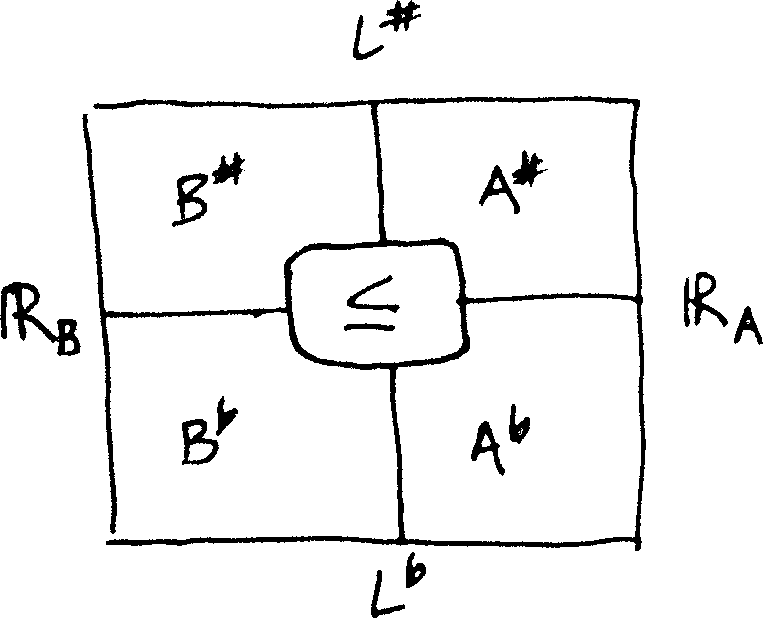
\includegraphics[scale=0.085]{draftfig/simsd}} }
\]
Simulation conventions are relational in nature.
Given $\mathbf{R} : A \leftrightarrow B$ and
$\mathbf{R}' : B \leftrightarrow C$,
we can derive their sequential composition
$\mathbf{R} \cdot \mathbf{R}' : A \leftrightarrow C$.
We will write $\epsilon_A : A \leftrightarrow A$
for the identity simulation convention,
and call $\mathbf{SC}$ the associated category of
language interfaces and simulation conventions.

%}}}

\begin{figure} % fig:overview:simcomp %{{{
  \[
      \pi_1 :
        L_1^\sharp
        \le_{\mathbf{R}_B \cdot \mathbf{R}_B' \twoheadrightarrow
             \mathbf{R}_C}
        L_1^\flat
      \qquad
      \pi_2 :
        L_2^\sharp
        \le_{\mathbf{R}_A \twoheadrightarrow \mathbf{R}_B}
        L_2^\natural
      \qquad
      \pi_2' :
        L_2^\natural
        \le_{\mathbf{R}_A' \twoheadrightarrow \mathbf{R}_B'}
        L_2^\flat
  \]
  \[
    \begin{tikzcd}[row sep=1.5em]
      A^\sharp \ar[r, twoheadrightarrow, "L_2^\sharp"]
	       \ar[d, leftrightarrow, "\mathbf{R}_A"'] &
      B^\sharp \ar[r, twoheadrightarrow, "L_1^\sharp"]
               \ar[d, leftrightarrow, "\mathbf{R}_B"] &
      C^\sharp \ar[dd, leftrightarrow, "\mathbf{R}_C"]
      \\
      A^\natural \ar[r, twoheadrightarrow, "L_2^\natural"]
	       \ar[d, leftrightarrow, "\mathbf{R}'_A"'] &
      B^\natural \ar[d, leftrightarrow, "\mathbf{R}'_B"]
      \\
      A^\flat \ar[r, twoheadrightarrow, "L_2^\flat"] &
      B^\flat \ar[r, twoheadrightarrow, "L_1^\flat"] &
      C^\flat
    \end{tikzcd}
    \qquad
    \begin{prooftree}
      \hypo{\pi_1 \quad}
      \hypo{\pi_2 \quad}
      \hypo{\quad \pi_2'}
      \infer2{
	%\pi_2 \odot \pi_2' :
	L_2^\sharp
	\le_{\mathbf{R}_A \cdot \mathbf{R}_A' \twoheadrightarrow
	     \mathbf{R}_B \cdot \mathbf{R}_B'}
	L_2^\flat}
      \infer2{
	%\pi_1 \otimes (\pi_2 \odot \pi_2') :
	L_1^\sharp \odot L_2^\sharp
	\le_{\mathbf{R}_A \cdot \mathbf{R}_A' \twoheadrightarrow
	     \mathbf{R}_C}
	L_1^\flat \odot L_2^\flat}
    \end{prooftree}
    \qquad
    \vcenter{ \hbox{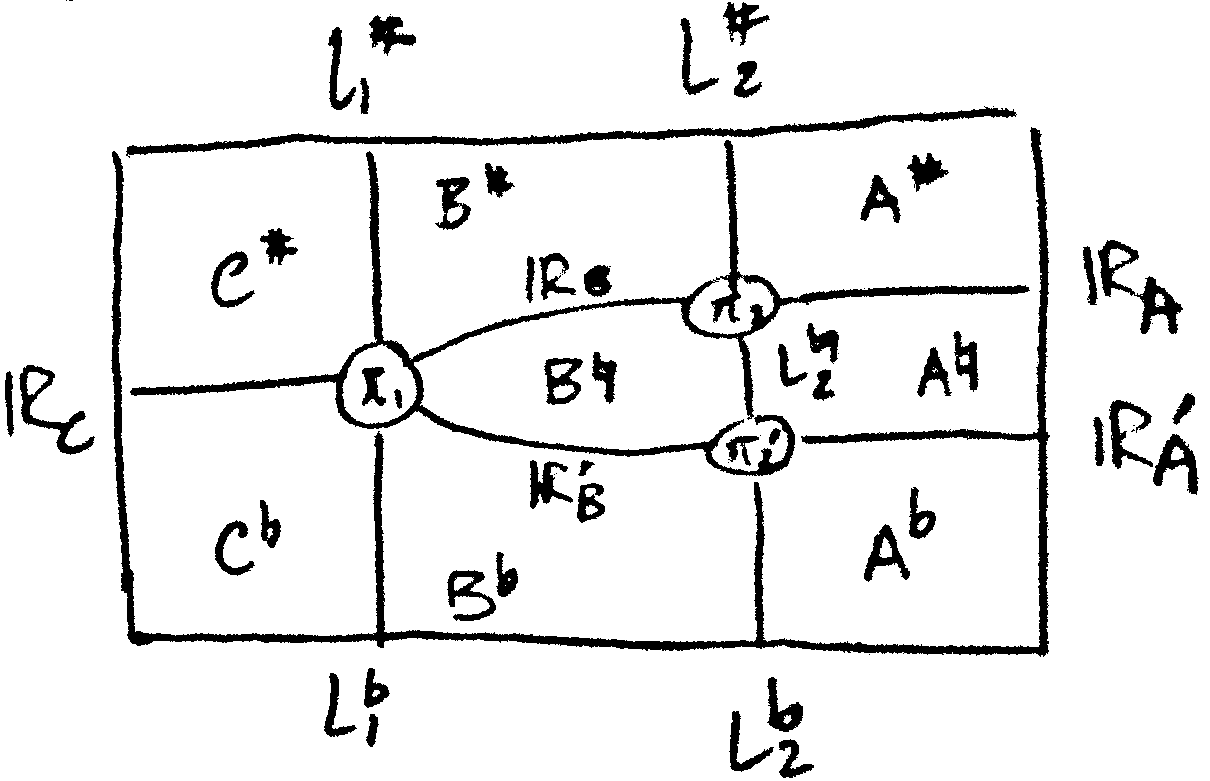
\includegraphics[scale=0.1]{draftfig/simsdcomp}} }
  \]
  \caption{A composite simulation proof
     and associated graphical representations}
  \label{fig:overview:simcomp}
\end{figure}
%}}}

\paragraph{Composition Properties} \label{sec:overview:doublecat} %{{{

As illustrated in Fig.~\ref{fig:overview:simcomp},
when their boundaries are compatible,
simulation squares of the kind depicted above compose both
vertically and horizontally.
Vertical composition produces a simulation
with composite incoming and outgoing simulation conventions.
Horizontal composition produces a simulation
between composite source and target components.

As suggested in \citet{compcerto},
given our use of $\odot$ as horizontal composition,
the composition properties outlined above
equip language interfaces,
transition systems and
simulation conventions
with the structure of a double category.
Compared with CompCertO,
we also make simulation conventions more expressive
by allowing them to retain a form of \emph{state},
so that they can relate successive interactions
in different ways.
Finally,
based on the $\mathbin@$ construction introduced in \S\ref{sec:overview:slift},
we add one more dimension to the compositional structure.

%}}}

%}}}

\subsection{Monoidal Structures} \label{sec:overview:mon} %{{{

We introduced in \S\ref{sec:overview:slift}
the constructions $A \mathbin@ U$ and $L \mathbin@ U$
which extend a language interface $A$ and a transition system $L$
with an additional state component taken in the set $U$.
This construction can be decomposed further
and extended to simulation conventions.

\begin{definition}[Composite language interfaces] \label{def:litens} %{{{
Given two language interfaces $A$ and $B$,
the language interface $A \otimes B$ is defined as:
$
  A \otimes B :=
    \langle A^\que \times B^\que, \,
            A^\ans \times B^\ans \rangle
$.
The language interface
$\mathbf{I} = \langle \mathbbm{1}, \mathbbm{1} \rangle$
is a unit for $\otimes$.
In addition, for a set $U$
we define the language interface
$[U] := \langle U, U \rangle$.
\end{definition}
%}}}

We can recover
$A \mathbin@ U := A \otimes [U]$.
Note also that $\otimes$ is %(in essence)
associative and commutative,
and that:
\[
  [U \times V] = [U] \otimes [V]
  \qquad \qquad
  [\mathbbm{1}] = \mathbf{I}
  \qquad
  [\varnothing] = \top
\]
Moreover,
these structures
are mirrored at the level of simulation conventions.

\paragraph{Simulation Conventions} %{{{

Two simulation conventions
$\mathbf{R} : A^\sharp \leftrightarrow A^\flat$ and
$\mathbf{S} : B^\sharp \leftrightarrow B^\flat$
can be combined into %a simulation convention
$
  \mathbf{R} \otimes \mathbf{S} :
  A^\sharp \otimes B^\sharp \leftrightarrow
  A^\flat \otimes B^\flat
$.
This simulation convention
(Def.~\ref{def:sctens})
requires the $A$ and $B$ components
of questions and answers
to be related independently by $\mathbf{R}$ and $\mathbf{S}$.
In addition,
a relation $R \subseteq U^\sharp \times U^\flat$
can be promoted to a simulation convention
$
  [R] : [U^\sharp] \leftrightarrow [U^\flat]
$
which uses $R$ as the underlying relation for both
questions and answers.

%}}}

\begin{example}[Correctness of \kw{bq.c}] \label{ex:bqcorrect} %{{{
Building on Example~\ref{ex:abspeclift},
consider the refinement between
\[
  L_\kw{bq} :
    \top \twoheadrightarrow \mathcal{C}@D_\kw{bq}
  \qquad\text{and}\qquad
  (\Sigma_\kw{bq} \mathbin@ D_\kw{rb}) \odot L_\kw{rb} :
    \top \twoheadrightarrow \mathcal{C}@D_\kw{rb}
  \,.
\]
To establish a simulation between them,
we use the abstraction relation
$R \subseteq D_\kw{bq} \times D_\kw{rb}$
defined by
\begin{align*}
  \vec{q} \mathrel{R} (b, c_1, c_2) \:\Leftrightarrow\: {}
    & (c_1 \le c_2 < N \:\wedge\: \vec{q} = b_{c_1} \cdots b_{c_2-1}) \vee {} \\
    & (c_2 \le c_1 < N \:\wedge\: \vec{q} = b_{c_1} \cdots b_{N-1} b_0 \cdots b_{c_2 - 1})
  \,.
\end{align*}
to formulate the correctness property
$
  \pi_\kw{bq} :
  L_\kw{bq}
  \:\le_{\top \twoheadrightarrow \mathcal{C} \otimes [R]}\:
  (\Sigma_\kw{bq} \mathbin@ D_\kw{rb}) \odot
  L_\kw{rb}
$.
\end{example}
%}}}

\paragraph{Categorical Structure} %{{{

These constructions satisfy many properties
which are well-understood in the context of category theory.
For example, the properties
\[
  \epsilon_A \otimes \epsilon_B = \epsilon_{A \otimes B}
  \qquad \text{and}
  \qquad
  (\mathbf{R}_1 \otimes \mathbf{R}_2) \cdot
  (\mathbf{S}_1 \otimes \mathbf{S}_2) =
  (\mathbf{R}_1 \cdot \mathbf{S}_1) \otimes
  (\mathbf{R}_2 \cdot \mathbf{S}_2)
  \,,
\]
and various properties of the invertible simulation conventions:
\[
  \lambda_A : A \otimes \mathbf{I} \cong A \,,
  \qquad
  \alpha_{ABC} : (A \otimes B) \otimes C \cong A \otimes (B \otimes C) \,,
  \qquad
  \gamma_{AB} : A \otimes B \cong B \otimes A \,,
\]
equip %the category
$\mathbf{SC}$
%of language interfaces and simulation conventions
with the structure of a \emph{symmetric monoidal category}.
Likewise, the properties
\[
  [{=}_U] = \epsilon_{[U]} \,,
  \qquad
  [R \cdot S] = [R] \mathbin; [S] \,,
  \qquad
  [R \times S] = [R] \otimes [S]
\]
can be captured by describing
$[-] : \mathbf{Rel} \rightarrow \mathbf{SC}$
as a \emph{monoidal functor}
from the symmetric monoidal category $\mathbf{Rel}$
of sets and relations
to the symmetric monoidal category $\mathbf{SC}$.

%This categorical description %of the compositional structure
%of simulation conventions
%brings with it useful tools.
%In essence,
Symmetric monoidal categories capture
the algebra of systems or processes which
compose both in series and parallel
\cite{rosetta}.
In the case of simulation conventions,
the process is one of concretization
from a high-level, abstract representation
of component interactions
to a more concrete and low-level one.
Series composition ($\cdot$)
allows us to carry out this process in a stepwise manner,
while parallel composition ($\otimes$)
allows us to operate independently on various components
of questions and answers.
This intuition is backed by the formal language of string diagrams.

%}}}

\paragraph{String Diagrams} %{{{

As implied by the properties above,
a composite morphism in a symmetric monoidal category
can often be written in a variety of equivalent ways.
String diagrams provide a more economical representation,
where these equivalences are captured
by simple geometric intuition.
For example, consider the following situation:
\[
  \begin{prooftree}
    \hypo{
      \begin{array}{c}
	w : A \leftrightarrow B \\
	x : \mathbf{I} \leftrightarrow C \\
	y : C \leftrightarrow D \\
	z : B \otimes D \leftrightarrow E
      \end{array}
    }
    \infer1{\mathbf{R} : A \leftrightarrow E}
  \end{prooftree}
  \quad
  \begin{array}{r@{}l}
    \mathbf{R} := {} &
    \lambda_A^{-1} \cdot
    (A \otimes x) \cdot
    (w \otimes y) \cdot
    z 
    \\[0.5ex]
    = {} &
    \lambda_A^{-1} \cdot
    (w \otimes (x \cdot y)) \cdot z
    \\[0.5ex]
    = {} &
    w \cdot \lambda_B^{-1} \cdot
    (B \otimes (x \cdot y)) \cdot z
    \\
    \vdots \:\, &
  \end{array}
  \qquad\qquad
  \mathbf{R} := \:\vcenter{\hbox{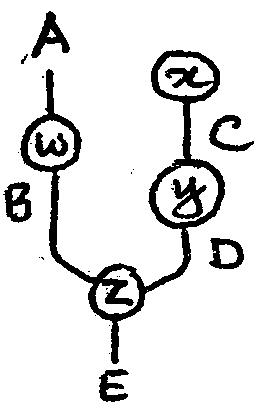
\includegraphics[scale=0.15]{draftfig/sdexample}} }
\]
Here,
we define a simulation convention $\mathbf{R}$ from various components
using categorical operations.
On the left,
we show the type of every variable,
and give several equivalent definitions for $\mathbf{R}$.
The string diagram on the right
captures the same information.
Note that
string diagrams
are \emph{formal} diagrams
which denote a particular morphism
with the same rigor
as traditional notation.

The string diagrams we use to represent simulation conventions
can be read from top to bottom.
Vertical lines denote language interfaces,
and horizontal juxtaposition represent tensor products.
Since it is the unit for $\otimes$,
the language interface $\mathbf{I}$ is not explicitly represented.
Nodes connect a group of lines above to a group of lines below
and denote elementary simulation conventions,
and are connected vertically to denote sequential composition.
Like the language interface $\mathbf{I}$,
the identity simulation convention $\epsilon$ is omitted,
and may appear as a vertical line without an intervening node.
Based on these conventions,
the string diagram above can be read as:
\newcommand{\chunk}[1]{%
  \vcenter{\hbox{%
    \includegraphics[scale=0.1]{draftfig/sd/#1}%
  }}%
}
\begin{align*}
  \mathbf{R}
     = \chunk{l1} \cdot \chunk{l2} \cdot \chunk{l3}
    &= \lambda_A^{-1} \cdot
       \left( \chunk{c1} \otimes \chunk{c2} \right) \cdot
       \left( \chunk{c3} \otimes \chunk{c4} \right) \cdot
       \chunk{c5} \\
    &= \lambda_A^{-1} \cdot (\epsilon_A \otimes x) \cdot (w \otimes y) \cdot z
    \,.
\end{align*}
%There are other ways to decompose the diagram,
%which yield some of the alternate formulas for $\mathbf{R}$
%shown above.
%But conversely,
%the string diagrams representations of these formulas
%are all identical,
%up to topological deformations
%which correspond to the axioms of monoidal categories.

%}}}

\paragraph{Transition Systems} %{{{

Unfortunately,
it is not possible in general
to form the tensor product of transition systems.
To see why, consider a hypothetical product
\[
  L_1 \otimes L_2 : A_1 \otimes A_2 \twoheadrightarrow B_1 \otimes B_2
  \,.
\]
When a question is received in $B_1 \otimes B_2$,
its components in $B_1$ and $B_2$ can be used to activate
the underlying transition systems $L_1$ and $L_2$.
However, during their execution,
each may ask
an arbitrary number of questions in $A_1$ and $A_2$.
In general,
there is no reason to expect that these questions
will synchronize or
that there will be a way to
combine them meaningfully
into questions of $A_1 \otimes A_2$.

Nevertheless,
it possible to generalize the construction $L@U$
introduced in \S\ref{sec:overview:slift}
to incorporate a \emph{lens} $f : U \lensarrow V$
with a more sophisticated action on the state component.
Such a lens provides access to a filed of type $U$ within $V$,
in the form of two functions:
\[
  \begin{array}{c}
    \kw{get}_f : V \rightarrow U \\[1ex]
    \kw{set}_f : V \times U \rightarrow V
  \end{array}
  \qquad
  \text{such that}
  \qquad
  \begin{array}{r@{\:}l}
    \kw{get}(\kw{set}(v, u)) &= u \\
    \kw{set}(v, \kw{get}(v)) &= v \\
    \kw{set}(\kw{set}(v, u_1), u_2) &= \kw{set}(v, u_2)
    \,.
  \end{array}
\]
The transition system
$L \mathbin@ f : A \mathbin@ U \rightarrow B \mathbin@ V$
can then use $\kw{get}_f$ to extract $u \in U$ from the incoming state in $V$,
thread that $U$ state component through the external calls of $L$,
and use $\kw{set}_f$ to update the state component of type $V$
in the top-level answer of $L$.

Sets and lenses form a category,
and the construction described above defines a functor
\[
  \mathbin@ : \mathbf{TS} \times \mathbf{Lens}
    \rightarrow \mathbf{TS}
  \,,
\]
which from $L : A \twoheadrightarrow B$
and $f : U \lensarrow V$
constructs
$
  L \mathbin@ f \::\: A \mathbin@ U \:\twoheadrightarrow\: B \mathbin@ V
$.
Since the right-hand side argument of $\mathbin@$
is limited to sets and lenses,
it cannot be used to define a proper monoidal structure on $\mathbf{TS}$.
Nevertheless, there are transition systems
\[
  \lambda_A : \mathbf{I} \mathbin@ U \cong [U]
  \qquad
  \rho_A : A \mathbin@ \mathbbm{1} \cong A
  \qquad
  \alpha_{AUV} : A \mathbin@ (U \times V) \cong
    (A \mathbin@ U) \mathbin@ V
\]
which satisfy a version of the expected properties.
This makes it possible to construct for transition systems
a string diagram language
similar to that of simulation conventions.

\begin{example}[Client code for $L_\kw{rb}$] %{{{
To compose $\kw{Clight}(\kw{bq.c})$ with $L_\kw{rb}$,
each must be extended with an additional state component.
This can be achieved in the following way:
\begin{gather*}
    XXX\vcenter{\hbox{ 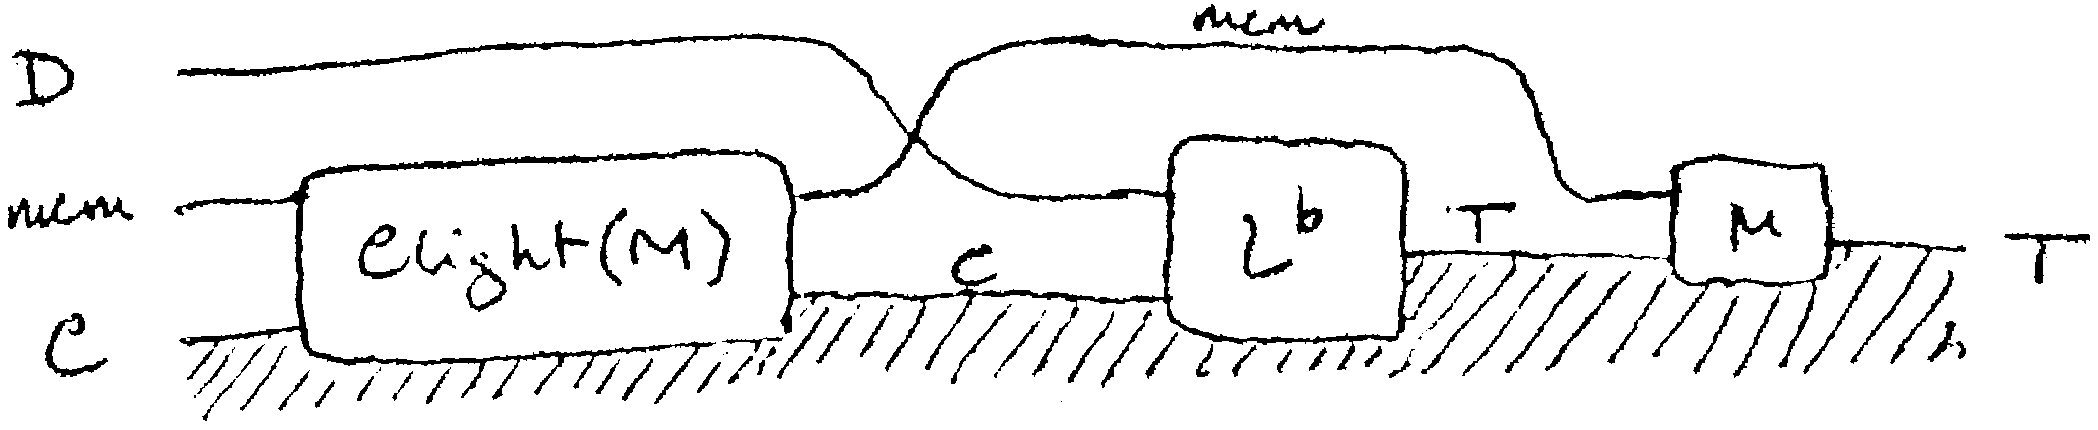
\includegraphics[scale=0.1]{draftfig/layersem-pure} }}XXX
  \\[1ex]
     (\kw{Clight}(\kw{bq.c}) \mathbin@ D_\kw{rb}) \odot
     (\mathcal{C} \mathbin@ \gamma_{\kw{mem}, D_\kw{rb}}) \odot
     (L_\kw{bq} \mathbin@ *_\kw{mem})
\end{gather*}
Composition runs from left to right
and the product
$\mathcal{C} \mathbin@ \kw{mem} \mathbin@ D_\kw{rb}$
run from bottom to top.
Lines and nodes connecting the shaded area
to the rest of the diagram
can be arbitrary language interfaces and transition systems,
but those appearing in the upper part
are restricted to sets and lenses.
We have drawn
$\gamma_{UV} : U \times V \lensarrow V \times U \in \mathbf{Lens}$
as a twist
and
${*}_U : \mathbbm{1} \lensarrow U$
as a circle.
\end{example}
%}}}

%}}}

%}}}

\subsection{Memory Separation} \label{sec:overview:sepalg} %{{{

The constructions we have outlined so far
make it possible to describe
the state of complex systems compositionally.
State can be separated into different fields;
we can then describe and reason about individual components
independently of the fields which they do not access,
and use the $\mathbin@$ operator
to connect these components with the rest of the system.

This compositional description
facilitates local reasoning,
but it must eventually be refined into
a concrete implementation:
a program acting on a global memory state
into which all state components have been merged.
To achieve this in a way which preserves compositionality,
we use a \emph{partial commutative monoid}
over the CompCert memory model.
This provides an operation $\bullet$
which can be used to decompose a memory state $m$ into
a number of \emph{shares}
$
  m_1 \bullet \cdots \bullet m_n
$.

The properties of $\bullet$
and its interaction with memory operations
ensure that CompCert semantics satisfy
a \emph{frame} property,
meaning that they are insensitive to
additional memory shares:
\begin{equation} \label{eqn:overview:sepalg:frame}
  \begin{prooftree}
  \hypo{
  L \:\vDash\: q@m_0 \rightarrowtail
    (q_1@m_1 \leadsto r_1@m_1') \rightarrowtail
    \cdots \rightarrowtail
    (q_n@m_n \leadsto r_n@m_n') \rightarrowtail
    r@m'}
  \infer1{
   {\begin{array}{r@{\:}l}
    L \:\vDash\: q@(m_0 \bullet w_0) \rightarrowtail
      \big( q_1@(m_1 \bullet w_0) &\leadsto r_1@(m_1' \bullet w_1) \big) \rightarrowtail
      \cdots \\ \cdots \rightarrowtail
      \big( q_n@(m_n \bullet w_{n-1}) &\leadsto r_n@(m_n' \bullet w_n) \big) \rightarrowtail
      r@(m' \bullet w_n)
   \end{array}} }
  \end{prooftree}
\end{equation}
The similarity of (\ref{eqn:overview:sepalg:frame})
with the behavior (\ref{eqn:slift})
of the transition system $L \mathbin@ U$ (\S\ref{sec:overview:slift})
is no coincidence.
In fact,
using the separation algebra as a relation
${\bullet} \subseteq (\kw{mem} \times \kw{mem}) \times \kw{mem}$,
the frame property for a transition system
$L : A \mathbin@ \kw{mem} \twoheadrightarrow B \mathbin@ \kw{mem}$
can be described as
$
  L \mathbin@ \kw{mem}
  \le_{A \otimes [\bullet] \twoheadrightarrow B \otimes [\bullet]}
  L
$.

The partial commutative monoid we use
is similar in spirit to the \emph{algebraic memory model}
of \citet{ccal};
its construction is explained in Appendix~\ref{sec:sep}.

%}}}

\subsection{ClightP} \label{sec:overview:clightp} %{{{

To further facilitate the implementation of abstract state,
we introduce the language
\[
  \kw{ClightP}(M) :
    \mathcal{C} \mathbin@ \kw{mem}
    \twoheadrightarrow
    \mathcal{C} \mathbin@ \kw{mem} \mathbin@ \kw{penv}
  \,,
\]
a variant of Clight
where global variables can be declared \emph{private}.
Private variables cannot be accessed
from other translation units and are stored
in a separate
\emph{private environment} $p \in \kw{penv}$.
The program $M$ can easily be compiled to a regular
Clight program $M' := \kw{ClightUnP}(M)$
by erasing the $\kw{private}$ annotations from all variables.
We will see in \S\ref{sec:clightp}
that the techniques presented in \S\ref{sec:overview:sepalg} 
play a key role in formulating the corresponding correctness property
for this transformation.

\begin{example}[Verifying $\kw{rb.c}$]
Using ClightP,
we can declare the variables
\texttt{c1}, \texttt{c2} and \texttt{buf}
as private.
We can then
define a relation $R_\kw{rb} \subseteq D_\kw{rb} \times \kw{penv}$
in order to verify
\[
  (\mathcal{C} \mathbin@ \gamma) \odot
  (L_\kw{rb} \mathbin@ \kw{mem})
  \le_{\varnothing \twoheadrightarrow \mathcal{C} \mathbin@ \kw{mem} \mathbin@ R_\kw{rb}}
  \kw{ClightP}(\kw{rb.c})
  \,.
\]
\end{example}

%}}}

\subsection{Encapsulated State} \label{sec:overview:encap} %{{{

In the semantic model of CompCertO, state exists in two forms:
\begin{itemize}
  \item The memory state is global and persistent.
    It is shared across all components
    and must be carried along
    every time a question or answer transfers control
    between components.
  \item The states used to define transition systems
    are local to each component.
    They can only be observed indirectly,
    through the component's interaction with the environment.
\end{itemize}
Since C does not offer objects, closures or similar abstractions,
component-local state has a lifetime limited to a particular function activation.
In the semantics of CompCert languages,
maintaining persistent local state
across successive activations of a given component
would serve no purpose.
Nevertheless,
persistent local state is important in many applications.

The constructions we have introduced so far
make it possible to manage global state
and control interference between components,
but do not support true encapsulation.
In \S\ref{sec:encap},
%we extend the semantic model of CompCertO
%to support to introduce \emph{persistent}
%local state.
%
%\paragraph{Approach}
%
%Rather than modifying the definition of transition systems,
we introduce a construction $\mathbf{C}^\dagger$
which can be applied to $\mathbf{TS}$ and $\mathbf{Lens}$
to obtain a model with state encapsulation.

%inspired by \citet{feedback,caots}.
%Concretely,
%a component $\Sigma : A \rightarrow B$
%consists of a set $U$ of \emph{private states},
%an underlying transition system of type
%$L : A \twoheadrightarrow B \mathbin@ U$,
%and an initial state $u \in U$.
%When $\Sigma$ is activated for the first time,
%the initial state is adjoined to incoming question
%to activate $L$.
%When $L$ terminates,
%the updated state is saved
%to be used with the next activation.

\paragraph{Encapsulation Primitive}

The double category structure
and the constructions we have described
embed into the extended model.
In addition,
that model supports a component:
\[
  \langle u \rangle : U \lensarrow \mathbbm{1} \in \mathbf{Lens}^\dagger
  \qquad
  \langle u \rangle := (u \in U \mid \rho^{-1}_U)
  =\:
  \draftfig{0.1}{encap-prim}
\]
This component is constructed from
$\rho^{-1}_U : U \cong \mathbbm{1} \times U \in \mathbf{Lens}$,
but the incoming $U$ component is hidden from its interface.
When the component is activated
by an incoming question $* \in \mathbbm{1}$,
the initial state $u \in U$ is adjoined
and propagated by $\rho^{-1}_U$ into an outgoing question.
When an answer $u' \in U$ is received
and propagated back by $\rho^{-1}_U$,
the component stores $u'$ as the next state and returns control to the environment.
This allows $\langle u \rangle$ to act
as a state encapsulation primitive.

\begin{example}[Encapsulated ClightP]
We define a version
$\kw{ClightP}\langle M \rangle :
    \mathcal{C} \mathbin@ \kw{mem} \rightarrow
    \mathcal{C} \mathbin@ \kw{mem}$
of the ClightP semantics
which encapsulates the private environment, as
\[
  \kw{ClightP} \langle M \rangle :=
  \:\draftfig{0.12}{encap-clightp}\: =
  (\mathcal{C} \mathbin@ \kw{mem} \mathbin@ \langle p_0 \rangle) \odot
    \kw{ClightP}(M)
  \,,
\]
where
$p_0 := \kw{init\_penv}(M)$
is the initial state of the private environment.
Note that the resulting type
means that ClightP semantics in this form
can be composed directly.
\end{example}

\paragraph{Simulations}

The component $\langle u \rangle$
has a \emph{companion}
$\langle u \rangle^* : [U] \leftrightarrow \mathbf{I}$
and a \emph{conjoint}
$\langle u \rangle_* : \mathbf{I} \leftrightarrow [U]$,
which are simulation conventions satisfying the simulation properties:
\begin{equation} \label{eqn:compconj}
  \draftfig{0.07}{comp1} \quad
  \draftfig{0.07}{comp2} \quad
  \draftfig{0.07}{conj1} \quad
  \draftfig{0.07}{conj2} \quad
  u \mathrel{R} v \Rightarrow
  \draftfig{0.1}{encap-rel}
\end{equation}
As shown above,
the simulation conventions $\langle u \rangle^*$
and $\langle u \rangle_*$
make it possible to relate components
where different amounts of state have been encapsulated.
The last property
establishes a form of representation independence
for encapsulated state.

%\begin{itemize}
%  \item Beyond the world of C,
%    many language features behave in this way.
%    It is important to understand how CompCertO's approach
%    carries over to this context.
%  \item For verification,
%    we want make it a structural thing
%    rather than a rely/guarantee property we carry around everywhere.
%    Example: certified abstraction layers.
%\end{itemize}
%In the remainder of this section,
%we show how persistent, encapsulated state
%can be incorporated into
%the semantic model of CompCertO.

%For the most part, the C language relies on a global memory state.
%Because all components can in principle access every part of this global memory,
%cross-component interactions carry the current state of the memory
%back and forth with every question and answer.

%}}}

%}}}

\section{A Double Category of Transition Systems} \label{sec:base} %{{{

% Preamble {{{

We begin our technical exposition with
our extensions to the semantic model of CompCertO.
While we reuse CompCertO's notion of transition system as-is,
we introduce our own layered composition operator.
Moreover,
our model makes simulation conventions and simulations
more general, so that they can account for
history-sensitive relationships
between source and target interactions.
After providing a formal description of this model,
we discuss its relationship with the original.

%}}}

\subsection{Transition Systems} \label{sec:base:ts} %{{{

As in the original CompCert semantics,
a transition system in CompCertO
executes by updating an internal state,
which is not directly observable
in its interactions with the environment.

\begin{definition} \label{def:lts} %{{{
A \emph{transition system} $L : A \twoheadrightarrow B$
is a tuple $L = \langle S, {\rightarrow}, I, X, Y, F \rangle$
consisting of:
\begin{itemize}
  \item a set $S$ of states;
  \item a transition relation ${\rightarrow} \subseteq S \times S$;
  \item a relation $I \subseteq B^\que \times S$
    which assigns possible \emph{initial states}
    to each question of $B$;
  \item a relation $F \subseteq S \times B^\ans$
    which specifies \emph{final states} together with
    corresponding answers in $B$;
  \item a relation $X \subseteq S \times A^\que$
    which identifies \emph{external states} and
    corresponding questions of $A$;
  \item a relation $Y \subseteq S \times A^\ans \times S$,
    which identifies \emph{resumption states}.
\end{itemize}
\end{definition}
%}}}

We use infix notation for the binary relations $I$, $F$, $X$.
We also write $r \mathrel{Y^s} s'$ when $(s, r, s') \in Y$;
this means that
after an external state $s$ triggers a question in $A^\que$ % ($s \mathrel{X} m$),
and the environment replies with an answer $r \in A^\ans$,
the execution resumes with state $s'$.
In other words,
the trace
\[
  q \rightarrowtail
  (q_1 \leadsto r_1) \rightarrowtail
  \cdots \rightarrowtail
  (q_n \leadsto r_n) \rightarrowtail
  r
\]
is generated by a transition sequence
\[
  q \mathrel{I} s_0 \rightarrow^*
  s_1 \mathrel{X} q_1 \leadsto
  r_1 \mathrel{Y^{s_1}} s_1' \rightarrow^*
  s_2 \mathrel{\cdots}
  s_n \mathrel{X} q_n \leadsto
  r_n \mathrel{Y^{s_n}} s_n' \rightarrow^*
  s_f \mathrel{F} r
\]

Note that
when $L : A \twoheadrightarrow B$
performs an outgoing call in $A$,
the internal state $s$ is preserved
until an answer resumes the execution.
By contrast, in $B$
no state is preserved across invocations of $L$.
Each question $q \in B^\que$ initializes a fresh state $s$
such that $q \mathrel{I} s$
regardless of any previous calls. % made into $L$.

%\begin{example}[Clight semantics] \label{ex:base:clightsem} %{{{
%In Example~\ref{ex:overview:clightsem}
%we discussed the externally observable behavior
%of the transition system
%$\kw{Clight}(\kw{rb.c}) :
% \mathcal{C} \mathbin@ \kw{mem} \twoheadrightarrow
% \mathcal{C} \mathbin@ \kw{mem}$.
%The trace mentioned in that example
%is generated by a transition sequence of the form
%\[
%  \kw{inc1}()@m[\kw{c1} \mapsto 5]
%  \mathrel{I}
%  s_0 \rightarrow \cdots \rightarrow s_k
%  \mathrel{F}
%  5@m[\kw{c1} \mapsto 6]
%  \,.
%\]
%Likewise,
%our example for
%$\kw{Clight}(\kw{bq.c})$
%is generated by a transition sequence
%\begin{align*}
%  \kw{deq}()@m
%  \mathrel{I}
%  u_0 \rightarrow \cdots \rightarrow u_1
%  \mathrel{X}
%  \kw{inc1}()@m &\leadsto i@m'
%  \mathrel{Y^{u_1}}
%  u_2 \rightarrow \cdots \\ \cdots \rightarrow u_3
%  \mathrel{X}
%  \kw{get}(i)@m' &\leadsto v@m''
%  \mathrel{Y^{u_3}}
%  u_4 \rightarrow \cdots \rightarrow u_5
%  \mathrel{F}
%  v@m''
%  \,.
%\end{align*}
%\end{example}
%%}}}
%
%To model linking,
%CompCertO introduces an operator $\oplus$
%which lets transition systems interact
%by having them handle each other's external calls.
%Because this operator permits mutual recursion,
%it is limited to transition systems which perform
%their incoming and outgoing calls
%according to the same language interface:
%\[
%  {\oplus_A} :
%    (A \twoheadrightarrow A) \times
%    (A \twoheadrightarrow A) \rightarrow
%    (A \twoheadrightarrow A)
%\]
%When mutual recursion is not needed,
%we can instead use the operator
%\[
%  {\odot_{A,B,C}} :
%    (B \twoheadrightarrow C) \times
%    (A \twoheadrightarrow B) \rightarrow
%    (A \twoheadrightarrow C)
%  \,,
%\]
%which is simpler in its construction
%and handles more general types.

\begin{definition}[Transition system composition] \label{def:lcomp} %{{{
The transition system
$\kw{id}_A : A \twoheadrightarrow A$
is defined as
\[
  \kw{id}_A \::=\:
  \big\langle
    A^\que + A^\ans, \:
    \varnothing, \:
    \iota_1, \:
    \iota_1^{-1}, \:
    \iota_2, \:
    \iota_2^{-1}
  \big\rangle
  \,.
\]
The composition of
$
  L_1 = \langle S_1, {\rightarrow_1}, I_1, X_1, Y_1, T_1 \rangle
    : B \twoheadrightarrow C
$ and $
  L_2 = \langle S_2, {\rightarrow_2}, I_2, X_2, Y_2, T_2 \rangle
    : A \twoheadrightarrow B
$,
is the transition system
$
  L_1 \odot L_2 :=
  \langle S, {\rightarrow}, I, X, Y, F \rangle
  : A \twoheadrightarrow C
$ defined as follows.
States are taken in the set
$
    S := S_1 + (S_2 \times S_1)
$.
When an call in $C$ activates $L_1$,
the left summand is used:
\[
  \begin{prooftree}
    \hypo{q_C \mathrel{I_1} s_1}
    \infer1{q_C \mathrel{I} \iota_1(s_1)}
  \end{prooftree}
  \qquad
  \begin{prooftree}
    \hypo{s_1 \rightarrow_1 s_1'}
    \infer1{\iota_1(s_1) \rightarrow \iota_1(s_1')}
  \end{prooftree}
  \qquad
  \begin{prooftree}
    \hypo{s_1 \mathrel{F_1} r_C}
    \infer1{\iota_1(s_1) \mathrel{F} r_C}
  \end{prooftree}
\]
When $L_1$ makes an outgoing call in $B$,
its current state is saved and
the question activates $L_2$.
The execution then
operates on the state of $L_2$
until a final state of $L_2$ is reached
and $L_1$ is resumed:
\[
  \small
  \begin{prooftree}
    \hypo{s_1 \mathrel{X_1} q_B}
    \hypo{q_B \mathrel{I_2} s_2}
    \infer2{\iota_1(s_1) \rightarrow \iota_2(s_2, s_1)}
  \end{prooftree}
  \quad
  \begin{prooftree}
    \hypo{s_2 \rightarrow_2 s_2'}
    \infer1{\iota_2(s_2, s_1) \rightarrow \iota_2(s_2', s_1)}
  \end{prooftree}
  \quad
  \begin{prooftree}
    \hypo{s_2 \mathrel{X_2} q_A}
    \infer1{\iota_2(s_2, s_1) \mathrel{X} q_A}
  \end{prooftree}
  \quad
  \begin{prooftree}
    \hypo{r_A \mathrel{Y_2^{s_2}} s_2'}
    \infer1{r_A \mathrel{Y^{\iota_2(s_2, s_1)}} \iota_2(s_2', s_1)}
  \end{prooftree}
  \quad
  \begin{prooftree}
    \hypo{s_2 \mathrel{F_2} r_B}
    \hypo{r_B \mathrel{Y_1^{s_1}} s_1'}
    \infer2{\iota_2(s_2, s_1) \rightarrow \iota_1(s_1')}
  \end{prooftree}
\]
\end{definition}
%}}}

%\begin{example} \label{ex:base:lcomp} %{{{
%Referring back to Example~\ref{ex:base:clightsem},
%consider the transition system:
%\[
%  \kw{Clight}(\kw{bq.c}) \odot \kw{Clight}(\kw{rb.c}) :
%  \mathcal{C}@\kw{mem} \twoheadrightarrow \mathcal{C}@\kw{mem}
%  \,.
%\]
%There,
%the calls of $\kw{bq.c}$ into $\kw{rb.c}$
%are turned into internal steps,
%triggering a switch between executions of the two components.
%For example,
%the call to $\kw{inc1}$ from $\kw{deq}$
%may proceed as follows:
%\begin{align*}
%  \kw{deq}()@m[\kw{c_1} \mapsto 5] \mathrel{I} \iota_1(u_0)
%  \rightarrow \cdots &\rightarrow \iota_1(u_1)
%  \rightarrow \iota_2(s_0, u_1)
%  \rightarrow \cdots \\ \cdots &\rightarrow \iota_2(s_k, u_1)
%  \rightarrow \iota_1(u_2) \rightarrow \cdots
%  \rightarrow \iota_1(u_5) \mathrel{F} v@m[\kw{c1} \mapsto 6]
%  \,.
%\end{align*}
%\end{example}
%%}}}

%}}}

\subsection{Kripke Relators} %{{{

To formulate our simulation infrastructure,
we will rely on the Kripke relator framework
used in \citet{compcerto},
which we summarize below.
Relators are operations on relations
which mirror operations on types.
They are similar to functors on $\mathbf{Rel}$
but satisfy weaker properties.

\paragraph{Basic Relators for Simulations}

Given two relations
$R \subseteq A \times B$ and
$S \subseteq U \times V$,
the relation
$(R \rightarrow S) \subseteq
 (A \rightarrow U) \times
 (B \rightarrow V)$
is defined in the usual way:
\[
  f \ifr{R \rightarrow S} g
  \quad:\Leftrightarrow\quad
  \forall (a, b) \in A \times B \mathbin.
    a \mathrel{R} b \Rightarrow
    f(a) \mathrel{S} g(b)
  \,.
\]
The more unusual powerset relator $\mathcal{P}^\le$
is used to express simulation diagrams.
Given $R \subseteq A \times B$,
the relation
$\mathcal{P}^\le(R) \subseteq \mathcal{P}(A) \times \mathcal{P}(B)$
is defined as:
\[
  x \ifr{\mathcal{P}^\le(R)} y
  \quad:\Leftrightarrow\quad
  \forall a \in x \mathbin.
  \exists b \in y \mathbin.
  a \mathrel{R} b
\]
To see how this works,
consider the simple transition systems
$\alpha : A \rightarrow \mathcal{P}(A)$
and
$\beta : B \rightarrow \mathcal{P}(B)$.
The relation $R$ is a simulation relation between them
when the following property holds:
\[
  \alpha \:\ifr{R \rightarrow \mathcal{P}^\le(R)}\: \beta
  \qquad\qquad\qquad
  \begin{tikzcd}
    a \ar[r, "\alpha"] \ar[d, dash, "R"'] &
    a' \ar[d, dash, dashed, "R"] \\
    b \ar[r, dashed, "\beta"'] &
    b'
  \end{tikzcd}
\]

\paragraph{Kripke Relations}

Components of complex data structures
must often be related in ways which vary
depending on the context in which they appear,
or the history of the computation.
In such cases,
component relations can be indexed over a set of \emph{worlds},
which capture the relevant contextual information.
Formally, a \emph{Kripke relation} over a set of worlds $W$
is a ternary relation $R \subseteq W \times A \times B$.
We will write $R \in \mathcal{R}_W(A, B)$,
and use the notation
$
  w \Vdash a \mathrel{R} b
$
to mean that $(w, a, b) \in R$.
We will also write
$\Vdash a \mathrel{R} b$
to mean that $a$ and $b$ are related at all worlds.

It is often useful to let the world evolve
by endowing $W$ with an \emph{accessibility} relation
${\leadsto} \subseteq W \times W$.
World transitions are then captured by the modal relator $\Diamond$,
which associates to a Kripke relation $R \in \mathcal{R}_W(A, B)$
the Kripke relation $\Diamond R$ of the same type, defined by:
\[
  w \Vdash a \ifr{\Diamond R} b
  \quad:\Leftrightarrow\quad
  \exists w' \mathbin. w \leadsto w' \wedge w' \Vdash a \mathrel{R} b
\]
For example,
a Kripke simulation between $\alpha : A \rightarrow \mathcal{P}(A)$
and $\beta : B \rightarrow \mathcal{P}(B)$
operating in the context of a Kripke frame $\langle W, {\leadsto} \rangle$
and a Kripke simulation relation $R \in \mathcal{R}_W(A, B)$
can be formulated in the following way.
The relators $\rightarrow$ and $\mathcal{P}^\le$
can be promoted to Kripke relators
by pointwise extension over the set of worlds.
The complex Kripke simulation property:
{\small
\[
  \forall w \in W \mathbin.
  \forall a \in A \mathbin.
  \forall b \in B \mathbin.
  w \Vdash a \mathrel{R} b \Rightarrow
  \forall a' \in \alpha(a) \mathbin.
  \exists b' \in \beta(b) \mathbin.
  \exists w' \in W \mathbin.
  w \leadsto w' \wedge w' \Vdash a' \mathrel{R} b'
\]
}
can be stated simply as
$
  \Vdash \alpha \ifr{R \rightarrow \mathcal{P}^\le(\Diamond R)} \beta
$.

%}}}

\subsection{Simulation Conventions} %{{{

Simulation conventions
characterize the relationship between
source- and target-level
questions and answers.
In CompCertO,
every pair of calls is related in isolation,
independently of any past or future calls.
Our notion of simulation convention
is more general,
and maintains state across calls.
%to operate on \emph{sequences} of calls.

\begin{remark}[Motivating stateful simulation conventions] \label{rem:base:ssc} %{{{
This will be useful in \S\ref{sec:encap}
when we introduce encapsulation.
Calls to a specification with encapsulated state
may produce traces like:
\begin{equation} \label{eqn:ssc:encap}
  \kw{inc}() \cdot 0 \cdot \kw{inc}() \cdot 1 \,\cdots {}
\end{equation}
However, a more concrete version (and eventually, the implementation)
may use explicit state:
\begin{equation} \label{eqn:ssc:explicit}
  \kw{inc}()@[\kw{c} \mapsto 0] \:\cdot\:
  0@[\kw{c} \mapsto 1] \:\cdot\:
  \kw{inc}()@[\kw{c} \mapsto 1] \:\cdot\:
  1@[\kw{c} \mapsto 2] \:\cdots\: {}
\end{equation}
The correspondence between
the questions and answers in (\ref{eqn:ssc:encap})
and those in (\ref{eqn:ssc:explicit})
cannot be formulated on a call-by-call basis
but must take into account the history of the computation.
\end{remark}
%}}}

State is maintained using Kripke worlds.
In CompCertO's version,
Kripke worlds are only used to ensure that
questions and answers for a given call
are related consistently.
We extend the definition to incorporate
caller and callee world transitions
as well as an initial world.

\begin{definition} \label{def:sconv} %{{{
A \emph{simulation convention}
$\mathbf{R} = \langle W, {\leadsto}, {\mapsto}, R^\que, R^\ans \rangle$
between %the language interfaces
$A^\sharp$ and $A^\flat$
is specified by:
\begin{itemize}
  \item a pointed set of worlds $W$,
    which store the current state of the simulation convention;
  \item a \emph{caller} accessibility relation ${\mapsto} \subseteq W \times W$;
  \item a \emph{callee} accessibility relation ${\leadsto} \subseteq W \times W$;
  \item a Kripke relation $R^\que \in \mathcal{R}_W\big(A_\sharp^\que,\, A_\flat^\que\big)$
    between the language interfaces' questions, and
  \item a Kripke relation $R^\ans \in \mathcal{R}_W\big(A_\sharp^\ans,\, B_\flat^\ans\big)$
    between their answers.
\end{itemize}
The accessibility relations are required to be reflexive and transitive.
We write $\mathbf{R} : A^\sharp \leftrightarrow A^\flat$.
\end{definition}
%}}}

\begin{example} \label{ex:base:ssc} %{{{
Referring to Remark~\ref{rem:base:ssc},
we can formulate a simulation convention
whose worlds capture the counter's value.
The callee may update it
but the caller must leave it unchanged.
\[
  \mathbf{R} := \langle \mathbb{N}, \top, {=}, R^\que, R^\ans \rangle
  \qquad
  \begin{prooftree}
    \infer0{n \Vdash \kw{inc}() \mathrel{R^\que} \kw{inc}()@[\kw{c} \mapsto n]}
  \end{prooftree}
  \qquad
  \begin{prooftree}
    \infer0{n + 1 \Vdash n \mathrel{R^\ans} n@[\kw{c} \mapsto n + 1]}
  \end{prooftree}
\]
The simulation convention $\mathbf{R}$ defined above
relates the sequences (\ref{eqn:ssc:encap}) and (\ref{eqn:ssc:explicit}).
\end{example}
%}}}

%The initial world $\intl{w}$ gives the simulation convention's initial state.
%While the environment is in control,
%the world may transition according to the relation $\mapsto$.
%When control is transferred to the system,
%the corresponding questions must be related by $w \Vdash R^\que$.
%World transitions may then occur according to $\leadsto$.
%Hence, when the system returns control to the environment,
%the corresponding answers
%will be related by $w' \Vdash R^\ans$,
%where $w'$ is a successor world of $w$ such that $w \leadsto w'$.
%The questions for any subsequent activation
%must in turn be related at a world $w''$ such that $w' \mapsto w''$,
%and so on and so forth indefinitely:
%\begin{align*}
%  \intl{w} \mapsto w_1 &\Vdash q^\sharp_1 \mathrel{R^\que} q^\flat_1 \\
%  w_1 \leadsto w_1' &\Vdash r^\sharp_1 \mathrel{R^\ans} r^\flat_1 \\
%  w_1' \mapsto w_2 &\Vdash q^\sharp_2 \mathrel{R^\que} q^\flat_2 \\
%  w_2 \leadsto w_2' &\Vdash r^\sharp_2 \mathrel{R^\ans} r^\flat_2 \\[-1ex]
%  &\:\:\vdots
%\end{align*}

\begin{definition}[Composition of Simulation Conventions] \label{def:sccomp}
The identity simulation convention
$\kw{id}_A : A \leftrightarrow A$
is given by
$\kw{id}_A := \langle
    \mathbbm{1}, {=}_\mathbbm{1}, {=}_\mathbbm{1}, {=}_{A^\que}, {=}_{A^\ans}
 \rangle$.
The simulation conventions
$\mathbf{R}_1 : A^\sharp \leftrightarrow A^\natural$ and
$\mathbf{R}_2 : A^\natural \leftrightarrow A^\flat$,
compose into
$\mathbf{R}_1 \mathbin; \mathbf{R}_2 : A^\sharp \leftrightarrow A^\flat$,
which is defined in the following way:
\begin{align*}
  W &:= W_1 \times W_2 &
  R^\que &:= R_1^\que \cdot R_2^\que &
  (w_1, w_2) \mapsto (w_1', w_2') \: &:\Leftrightarrow \:
    w_1 \mapsto_1 w_1' \: \wedge \:
    w_2 \mapsto_2 w_2' \\
&&  R^\ans &:= R_1^\ans \cdot R_2^\ans &
  (w_1, w_2) \leadsto (w_1', w_2') \: &:\Leftrightarrow \:
    w_1 \leadsto_1 w_1' \: \wedge \:
    w_2 \leadsto_2 w_2'
  \,.
\end{align*}
\end{definition}

%}}}

\subsection{Simulations} \label{sec:base:sim} %{{{

We are now ready to define our generalized notion of simulation.
Consider a simulation of type:
\[
\begin{tikzcd}
  A_1 \ar[r, twoheadrightarrow, "L_1"] \ar[d, leftrightarrow, "\mathbf{R}_A"'] &
  B_1 \ar[d, leftrightarrow, "\mathbf{R}_B"] \\
  A_2 \ar[r, twoheadrightarrow, "L_2"] & B_2
\end{tikzcd}
\]
The simulation simultaneously
plays the role of the caller with respect to
the simulation convention $\mathbf{R}_A$ and
the role of the callee with respect to $\mathbf{R}_B$.
Hence,
it will operate in the context of a Kripke frame
constructed from both $W_A$ and $W_B$.
The possible states of a simulation will be a subset
$W \subseteq W_A \times W_B$,
which must contain
the initial state $\intl{w} := (\intl{w}_A, \intl{w}_B) \in W$.
Between successive activations,
the environment may update the $W_B$ component.
Hence we require:
\[
  (w_A, w_B) \in W \:\wedge\:
  w_B \mapsto_B w_B' \:\Rightarrow\:
  (w_A, w_B') \in W
\]
When the components execute,
the worlds will evolve according to
the accessibility relation:
\[
  (w_A, w_B) \leadsto_{\bar{A}B} (w_A', w_B') \::\Leftrightarrow\:
  w_A \mapsto_A w_A' \:\wedge\: w_B \leadsto_B w_B'
\]
Reading the constituent transition relations
within $L_1, L_2$ as functions of type:
\begin{align*}
  I_1 &: B_1^\que \rightarrow \mathcal{P}(S_1) &
  {\rightarrow_1} &: S_1 \rightarrow \mathcal{P}(\mathbb{E}^* \times S_1) &
  F_1 &: S_1 \rightarrow \mathcal{P}(B_1^\ans)
  \\
  I_2 &: B_2^\que \rightarrow \mathcal{P}(S_2) &
  {\rightarrow_2} &: S_2 \rightarrow \mathcal{P}(\mathbb{E}^* \times S_2) &
  F_2 &: S_2 \rightarrow \mathcal{P}(B_2^\ans)
  \,,
\end{align*}
we can formulate the simulation properties for internal steps
as shown in \autoref{fig:simint}.

\begin{figure} % fig:simint {{{
  \small
  \[
    \begin{array}{c@{\qquad}c@{\qquad}c}
      \begin{tikzcd}[sep=tiny,column sep=0]
        q_1 \ar[dd, "w \Vdash \mathbf{R}_B^\que"', dash] \ar[rr, dash, "I_1"] &&
        s_1 \ar[dd, "w' \Vdash R", dash, dashed] \\
        & \leadsto_{\bar{A}B} & \\
        q_2 \ar[rr, "I_2"', dash, dashed] &&
        s_2
      \end{tikzcd}
      &
      \begin{tikzcd}[sep=tiny,column sep=0]
        s_1 \ar[rr, "t"] \ar[dd, "w \Vdash R"', dash] &&
        \!\!{}_1 \:\, s_1' \ar[dd, "w' \Vdash R", dash, dashed] \\
        & \leadsto_{\bar{A}B} & \\
        s_2 \ar[rr, "t", dashed] &&
        \!\!{}_2^* \:\, s_2'
      \end{tikzcd}
%      \begin{tikzcd}[sep=large]
%        s_1 \ar[r] \ar[d, "{(w_A, w_B) \Vdash R}"', dash] &
%        s_1' \ar[d, "{(w_A,w_B) \Vdash R}", dash, dashed] \\
%        s_2 \ar[r, dashed] &
%        \!\!\!{}^* \: s_2'
%      \end{tikzcd}
      &
      \begin{tikzcd}[sep=tiny, column sep=0]
        s_1 \ar[rr, "F_1", dash] \ar[dd, "w \Vdash R"', dash] &&
        r_1 \ar[dd, "w' \Vdash \mathbf{R}_B^\ans", dash, dashed] \\
        & \leadsto_{\bar{A}B} & \\
        s_2 \ar[rr, "F_2"', dash, dashed] &&
        r_2
      \end{tikzcd}
      \vspace{1ex} \\
      I_1 \ifr{\Vdash \mathbf{R}_B^\que \rightarrow
        \mathcal{P}^\le(\Diamond_{\bar{A}B} R)} I_2
      &
      {\rightarrow_1}
      \ifr{\Vdash R \rightarrow \mathcal{P}^\le(\Diamond_{\bar{A}B} ({=} \times R))}
      {\rightarrow_2^*}
      &
      F_1
      \ifr{\Vdash R \rightarrow \mathcal{P}^\le(\Diamond_{\bar{A}B} \mathbf{R}_B^\ans)}
      F_2
      \vspace{1.2ex} \\
      \text{(a) Initial states} &
      \text{(b) Internal states} &
      \text{(c) Final states}
    \end{array}
  \]
  \caption{Stateful simulation properties for internal steps}
  \label{fig:simint}
\end{figure}
%}}}

Conversely, for external calls,
the simulation plays the role of the environment.
We expect that:
\[
  (w_A, w_B) \in W \:\wedge\:
  w_A \leadsto_A w_A' \:\Rightarrow\:
  (w_A', w_B) \in W
\]
Moreover,
from the point of view of the simulation,
an external call will make a transition according to
the following accessibility relation:
%[NB we may want to restrict $\leadsto_B$ to $=$
%if this causes problems, but]
%Note that by allowing a transition $w_B \leadsto_B w_B'$,
%we are able to capture the effect that
%any reentrant call may have on the simulation state:
\[
  (w_A, w_B) \leadsto_{AB} (w_A', w_B') \::\Leftrightarrow\:
  w_A \leadsto_A w_A' \:\wedge\:
  w_B = w_B'
\]
By reading the action of transition systems at external calls
in terms of the functions:
\begin{align*}
  Z_1 &: S_1 \rightarrow
    \mathcal{P}(A_1^\que \times (A_1^\ans \rightarrow \mathcal{P}(S_1))) &
  Z_1(s_1) &:= \{ (q_1, Y_1^{s_1}) \mid s_1 \mathrel{X_1} q_1 \}
 \\
  Z_2 &: S_2 \rightarrow
    \mathcal{P}(A_2^\que \times (A_2^\ans \rightarrow \mathcal{P}(S_2))) &
  Z_2(s_2) &:= \{ (q_2, Y_2^{s_2}) \mid s_2 \mathrel{X_2} q_2 \}
  \,,
\end{align*}
we can then formulate the simulation condition for external calls
as presented in \autoref{fig:simext}.

\begin{figure} % fig:simext {{{
  \[
    \begin{array}{c}
      \begin{tikzcd}[sep=tiny, column sep=small]
        s_1 \ar[rr, "X_1", dash] \ar[dd, "w \Vdash R"', dash] &&
        m_1 \ar[rr, dotted, dash] \ar[dd, "w'"', "{} \Vdash \mathbf{R}_A^\que", dash, dashed] &&
        n_1 \ar[rr, "Y_1^{s_1}", dash] \ar[dd, "w''"', "{} \Vdash \mathbf{R}_A^\ans", dash] &&
        s_1' \ar[dd, "w''' \Vdash R", dash, dashed]
        \\
        & \leadsto_{\bar{A}B} && \leadsto_{AB} && \leadsto_{\bar{A}B} &
        \\
        s_2 \ar[rr, "X_2"', dash, dashed] &&
        m_2 \ar[rr, dotted, dash] &&
        n_2 \ar[rr, "Y_2^{s_2}"', dash, dashed] &&
        s_2'
      \end{tikzcd}
      \vspace{1ex} \\
      Z_1
      \mathrel{[
        \Vdash R \rightarrow \mathcal{P}^\le(
          \Diamond_{\bar{A}B} (
          \mathbf{R}_A^\que \times
            \Box_{AB} (
            \mathbf{R}_A^\ans \rightarrow
            \mathcal{P}^\le(\Diamond_{\bar{A}B} R))))
      ]}
      Z_2
    \end{array}
  \]
  \caption{Simulation property for external states}
  \label{fig:simext}
\end{figure}
%}}}

\begin{definition}[Open simulation]
There is a simulation
of $L_1 : A_1 \twoheadrightarrow B_1$
by $L_2 : A_2 \twoheadrightarrow B_2$
under the simulation conventions
$\mathbf{R}_A : A_1 \leftrightarrow A_2$ and
$\mathbf{R}_B : B_1 \leftrightarrow B_2$,
if there exists
\begin{itemize}
\item a set of worlds $W$,
closed under ${\leadsto_A} \times {\mapsto_B}$ and
such that
$(\intl{w}_A, \intl{w}_B) \in W \subseteq W_A \times W_B$;
and
\item
a Kripke relation $R \in \mathcal{R}_W(S_1, S_2)$
between the states of $L_1$ and $L_2$;
\end{itemize}
satisfying the properties given in
\autoref{fig:simint} and
\autoref{fig:simext}.
We will write
$L_1 \preceq_{\mathbf{R}_A \twoheadrightarrow \mathbf{R}_B} L_2$.
\end{definition}

%}}}

\subsection{Compositional Structure} \label{sec:base:double} %{{{

The composition of transitions systems and simulation conventions
define the respective categories $\mathbf{TS}$ and $\mathbf{SC}$.
In addition,
simulations compose both horizontally and vertically,
namely:
\[
  \begin{prooftree}
    \hypo{
      L_1^\sharp
      \preceq_{\mathbf{R}_B \twoheadrightarrow \mathbf{R}_C}
      L_1^\flat}
    \hypo{
      L_2^\sharp
      \preceq_{\mathbf{R}_A \twoheadrightarrow \mathbf{R}_B}
      L_2^\flat}
    \infer2{
      L_1^\sharp \odot L_2^\sharp
      \preceq_{\mathbf{R}_A \twoheadrightarrow \mathbf{R}_C}
      L_1^\flat \odot L_2^\flat}
  \end{prooftree}
  \qquad
  \begin{prooftree}
    \hypo{L^\sharp
      \preceq_{\mathbf{R}_A \twoheadrightarrow \mathbf{R}_B}
      L^\natural}
    \hypo{L^\natural
      \preceq_{\mathbf{S}_A \twoheadrightarrow \mathbf{S}_B}
      L^\flat}
    \infer2{L^\sharp
      \preceq_{\mathbf{R}_A \mathbin; \mathbf{S}_A \twoheadrightarrow
	   \mathbf{R}_B \mathbin; \mathbf{S}_B}
      L^\flat}
  \end{prooftree}
\]
Overall,
the compositional structure of our model
can be stated concisely in the following way.

\begin{theorem}
Language interfaces,
transition systems,
simulation conventions and
simulation properties
form a thin double category $\mathbf{TSC}$.
\end{theorem}

This characterization
gives a formal underpinning to the usual notions of
horizontal and vertical composition
found in existing work on compositional certified compilers.

%\begin{lemma}[Horizontal composition of simulations]
%\[
%  \begin{prooftree}
%    \hypo{
%      L_1^\sharp
%      \preceq_{\mathbf{R}_B \twoheadrightarrow \mathbf{R}_C}
%      L_1^\flat}
%    \hypo{
%      L_2^\sharp
%      \preceq_{\mathbf{R}_A \twoheadrightarrow \mathbf{R}_B}
%      L_2^\flat}
%    \infer2{
%      L_1^\sharp \odot L_2^\sharp
%      \preceq_{\mathbf{R}_A \twoheadrightarrow \mathbf{R}_C}
%      L_1^\flat \odot L_2^\flat}
%  \end{prooftree}
%  \qquad \qquad
%  \begin{tikzcd}
%    A^\sharp \ar[r, twoheadrightarrow, "L_2^\sharp"]
%	     \ar[d, leftrightarrow, "\mathbf{R}_A"] &
%    B^\sharp \ar[r, twoheadrightarrow, "L_1^\sharp"]
%	     \ar[d, leftrightarrow, "\mathbf{R}_B"] &
%    C^\sharp \ar[d, leftrightarrow, "\mathbf{R}_C"]
%    \\
%    A^\flat \ar[r, twoheadrightarrow, "L_2^\flat"'] &
%    B^\flat \ar[r, twoheadrightarrow, "L_1^\flat"'] &
%    C^\flat
%  \end{tikzcd}
%\]
%\end{lemma}
%
%\begin{theorem}[Vertical composition of simulations] \label{thm:svcomp}
%\[
%  \begin{prooftree}
%    \hypo{L^\sharp
%      \preceq_{\mathbf{R}_A \twoheadrightarrow \mathbf{R}_B}
%      L^\natural}
%    \hypo{L^\natural
%      \preceq_{\mathbf{S}_A \twoheadrightarrow \mathbf{S}_B}
%      L^\flat}
%    \infer2{L^\sharp
%      \preceq_{\mathbf{R}_A \mathbin; \mathbf{S}_A \twoheadrightarrow
%	   \mathbf{R}_B \mathbin; \mathbf{S}_B}
%      L^\flat}
%  \end{prooftree}
%\]
%\end{theorem}
%
%\begin{theorem}[Layered composition of simulations] \label{thm:lcompsim}
%Simulations compose as follows:
%\[
%  \begin{prooftree}
%    \hypo{L_1^\sharp
%          \le_{\mathbf{R}_B \twoheadrightarrow \mathbf{R}_C}
%          L_1^\flat}
%    \hypo{L_2^\sharp
%          \le_{\mathbf{R}_A \twoheadrightarrow \mathbf{R}_B}
%          L_2^\flat}
%    \infer2{L_1^\sharp \odot L_2^\sharp
%          \le_{\mathbf{R}_A \twoheadrightarrow \mathbf{R}_C}
%          L_1^\flat \odot L_2^\flat}
%  \end{prooftree}
%  \qquad \qquad
%  \begin{tikzcd}
%    A^\sharp \ar[r, twoheadrightarrow, "L_2^\sharp"]
%             \ar[d, Leftrightarrow, "\mathbf{R}_A"'] &
%    B^\sharp \ar[r, twoheadrightarrow, "L_1^\sharp"]
%             \ar[d, Leftrightarrow, "\mathbf{R}_B"] &
%    C^\sharp \ar[d, Leftrightarrow, "\mathbf{R}_C"]
%    \\
%    A^\flat \ar[r, twoheadrightarrow, "L_2^\flat"'] &
%    B^\flat \ar[r, twoheadrightarrow, "L_1^\flat"'] &
%    C^\flat
%  \end{tikzcd}
%\]
%\end{theorem}

%}}}

\subsection{Relationship with CompCertO} %{{{

The simulation conventions used in CompCertO
constitute a subset of the ones we have defined.
In CompCertO,
the caller may specify an arbitrary world with each new call.
The callee must relate the answers at the same world.
Hence,
within the context of our definition,
CompCertO's simulation conventions
take the form $\langle W, {=}, \top, R^\que, R^\ans \rangle$.

When simulation conventions of this form are used,
CompCertO's simulations coincide with our own,
making them possible to reuse within our framework.
In particular,
CompCertO's correctness theorem can be reused as-is,
and combined with any correctness result
obtained for Clight programs.

Moreover,
CompCertO defines a notion of simulation convention \emph{refinement},
whereby a simulation convention
can replace another in all simulation statments.
Having defined a proper categorical structure for $\mathbf{TS}$,
in our setting
it will be possible to encode simulation convention refinement as:
\[
  \mathbf{R} \sqsubseteq \mathbf{S} \quad :\Leftrightarrow \quad
    \kw{id} \le_{\mathbf{R} \rightarrow \mathbf{S}} \kw{id}
\]
The interaction of $\sqsubseteq$ with simulations properties
is then just an instance of horizontal composition.

Finally,
our layered composition operator $\odot$
\emph{under-approximates}
CompCertO's semantic linking operator $\oplus$.
Since CompCert's syntactic linking of assembly programs
is known to implement $\oplus$,
this shows that linking is also a correct implementation of
the layered composition $\odot$.

\begin{theorem}[Linking implements layered composition]
For two assembly programs $M_1, M_2$,
%For $L_1, L_2 : A \twoheadrightarrow A$,
\[
  \kw{Asm}(M_1) \odot \kw{Asm}(M_2)
  \le
  \kw{Asm}(M_1) \oplus \kw{Asm}(M_2)
 \,.
\]
\end{theorem}

This means that when a system is compositionally
specified and verified at the Clight level,
and an overall correctness property is derived
in terms of $\odot$,
we can combine it with the compiler's correctness theorem
to obtain guarantees about the linked assembly program.

%}}}

%}}}

\section{Compositional State} \label{sec:scomp} %{{{

The constructions described in \S\ref{sec:base}
equip CompCertO semantics
with the two-dimensional structure of a double category.
In this section,
we add one more dimension to our compositional infrastructure,
spanning different components of a system's state.

%building on the outline given in \S\ref{sec:overview:mon},
%We formalize these structures for
%transition systems (\S\ref{sec:base:tsmon}),
%and for simulations (\S\ref{sec:base:scmon}).
%
%We have mentioned in \S\ref{sec:base:compcerto}
%CompCertO's approach to \emph{state}:
%the internal states of transition systems
%cannot be observed across components and
%persist only for the duration of a function activation;
%therefore,
%every question and answer must be annotated with
%the current state of the global memory
%at the time of a function's invocation or return,
%as shown in the language interface $\mathcal{C}@\kw{mem}$
%discussed in Example~\ref{ex:langint}.
%
%In this section,
%we show how this overall approach to persistent state
%can be generalized,
%and we introduce constructions
%which can be used to manage
%this kind of global state.

\subsection{Bijections and Relations} %{{{

As we have noted in \S\ref{sec:overview:mon},
transition systems acting on independent components
of language interfaces
cannot in general be composed directly.
However,
transition systems can be extended to pass along
an additional state component,
possibly transformed between their incoming and outgoing interfaces
using a bijective function.
In fact, bijections and relations
form their own double category,
which embeds into $\mathbf{TSC}$.
The associated simulation property
is defined as follows.

\begin{definition}
Given two bijective functions
$f^\sharp : U^\sharp \rightarrow V^\sharp$ and
$f^\flat : U^\flat \rightarrow V^\flat$,
we say that there is a bisimulation of $f^\sharp$ by $f^\flat$
with respect to
$R_U \subseteq U^\sharp \times U^\flat$ and 
$R_V \subseteq V^\sharp \times V^\flat$
when:
\[
  \forall u^\sharp u^\flat \mathbin.
    \big( u^\sharp \mathrel{R_U} u^\flat \Leftrightarrow
     f^\sharp(u^\sharp) \mathrel{R_V} f^\flat(u^\flat) \big)
\]
We will write $f^\sharp \equiv_{R_U \cong R_V} f^\flat$.
\end{definition}

Simulations of this kind compose
both horizontally and vertically
so that sets,
bijective functions and
relations,
under their usual composition algebras,
constitute a thin double category
$\mathbf{SBR}$.
We will see that there is a double functor
$[-] : \mathbf{SBR} \hookrightarrow \mathbf{TSC}$
identifying $\mathbf{SBR}$ as a subcategory of $\mathbf{TSC}$.

%}}}

\subsection{Transition Systems} \label{sec:scomp:tr} %{{{

As explained in \S\ref{sec:overview:slift},
transition systems can be extended
to pass along an extra state component.
In addition,
a bijection can be used to translate
this extra state between incoming and outgoing calls.

\begin{definition}[Lifting] \label{def:lift} %{{{
Given a transition system
$L = \langle S, {\rightarrow}, I, X, Y, F \rangle : A \twoheadrightarrow B$
and a bijective function $f : U \rightarrow V$,
the transition system
$L \mathbin@ f : A \mathbin@ U \twoheadrightarrow B \mathbin@ V$
is defined as:
\begin{gather*}
  L \mathbin@ f := \langle S \times U, {\rightarrow_U}, I_U, X_U, Y_U, F_U \rangle \\
 {\begin{prooftree}
    \hypo{q \mathrel{I} s}
    \hypo{f^{-1}(v) = u}
    \infer2{q@v \mathrel{I_U} s@ u}
  \end{prooftree}}
  \quad
 {\begin{prooftree}
    \hypo{s \rightarrow s'}
    \infer1{s@u \rightarrow_U s'@u}
  \end{prooftree}}
  \quad
 {\begin{prooftree}
    \hypo{s \mathrel{X} m}
    \infer1{s@u \mathrel{X_U} m@u}
  \end{prooftree}}
  \quad
 {\begin{prooftree}
    \hypo{n \mathrel{Y}^s s'}
    \infer1{n@u' \mathrel{Y^{s@u}_U} s'@u'}
  \end{prooftree}}
  \quad
 {\begin{prooftree}
    \hypo{s \mathrel{F} r}
    \hypo{f(u) = v}
    \infer2{s@u \mathrel{F_U} r@v}
  \end{prooftree}}
\end{gather*}
\end{definition}
%}}}

\begin{theorem} %{{{
The operation defined above satisfies
defines a functor
${@} : \mathbf{TS} \times \mathbf{Bij} \rightarrow \mathbf{TS}$
since
\[
  (L_1 \odot L_2) \mathbin@ (f \circ g) \equiv
    (L_1 \mathbin@ f) \odot (L_2 \mathbin@ g)
  \,,
  \qquad
  \kw{id}_A \mathbin@ \kw{id}_U \equiv \kw{id}_{A \mathbin@ U}
  \,.
\]
This functor can be specialized to
$[-] : \mathbf{Bij} \rightarrow \mathbf{TS}$
by defining
$[f] := \kw{id}_\mathbf{I} \mathbin@ f$.
\end{theorem}
%}}}

%}}}

\subsection{Simulation Conventions} \label{sec:scomp:sc} %{{{

Compared with transition systems,
simulation conventions compose more easily.
They admit a fine-grained
composition structure
which follows the constructions introduced in Def.~\ref{def:litens}.

\begin{definition}[Tensor product of simulation conventions] \label{def:sctens}
Given $R_A : A^\sharp \leftrightarrow A^\flat$
and $R_B : B^\sharp \leftrightarrow B^\flat$,
we can define the simulation convention
$R_A \otimes R_B : A^\sharp \otimes B^\sharp
  \leftrightarrow
  A^\flat \otimes B^\flat$
as follows:
\[
  R_A \otimes R_B \: := \:
    \big\langle
      W_A \times W_B, \:
      R_A^\que \times R_B^\que, \:
      R_A^\ans \times R_B^\ans
    \big\rangle
\]
In addition,
given a relation $R \subseteq U \times V$,
the simulation convention $[R] : [U] \leftrightarrow [V]$
is defined as
\[
  [R] := \langle \mathbbm{1}, \top, \top, R, R \rangle
  \,.
\]
We will also write $\mathbf{R} \mathbin@ R := \mathbf{R} \otimes [R]$.
\end{definition}

%As outlined in \S\ref{sec:overview:mon},
%these constructions satisfy many pleasant properties,
%which can be summarized as follows.

\begin{theorem}
The constructions above constitute \emph{functors}
${\otimes} : \mathbf{SC} \times \mathbf{SC} \rightarrow \mathbf{SC}$
and
$[-] : \mathbf{Rel} \rightarrow \mathbf{SC}$.
$\mathbf{SC}$ under $\otimes$ is a symmetric monoidal category,
and $[-]$ is a monoidal functor
from $\langle \mathbf{Rel}, {\times} \rangle$ to
$\langle \mathbf{SC}, {\otimes} \rangle$.
\end{theorem}

%}}}

\subsection{Simulations} \label{sec:scomp:sim} %{{{

Finally,
the compositional structures we have introduced above
are compatible with simulations:
\[
  \begin{prooftree}
    \hypo{L^\sharp \le_{\mathbf{R} \twoheadrightarrow \mathbf{S}} L^\flat}
    \hypo{f \equiv_{R \cong S} g}
    \infer2{
      L^\sharp \mathbin@ f
      \:\le_{\mathbf{R}\mathbin@R \rightarrow \mathbf{S}\mathbin@S}\:
      L^\flat \mathbin@ g
    }
  \end{prooftree}
\]
This can be stated as follows.

\begin{theorem}
The constructions in this section
define a double functor
${@} : \mathbf{TSC} \times \mathbf{SBR} \rightarrow \mathbf{TSC}$
and a double functor
$[-] : \mathbf{SBR} \hookrightarrow \mathbf{TSC}$.
\end{theorem}

%}}}

%}}}

\section{Clight with module-local state} \label{sec:clightp} %{{{

We have briefly introduced in \S\ref{sec:overview:clightp}
the language ClightP which allows \emph{private} variables
to be stored in a separate environment.
We now discuss the correctness of
the transformation $\kw{ClightUnP}$
which converts private variables into regular variables
stored in the global memory state.
The corresponding correctness property is
formulated using the techniques outlined in \S\ref{sec:overview:sepalg}.

\subsection{Correctness Property}

Given a simulation convention $\mathbf{R} : A \leftrightarrow \kw{mem}$,
we write $\mathbf{R}^\bullet :=
(\kw{mem} \otimes \mathbf{R}) \mathbin; [\bullet] :
 \kw{mem} \otimes A \leftrightarrow \kw{mem}$
for the simulation convention
which merges the target memory share of $\mathbf{R}$
into another memory component.
In addition,
the simulation convention $[U]_* : \mathbf{I} \leftrightarrow U$
allows the caller to use an arbitrary target question $u$
but requires the callee to return it unchanged.
The correctness of $\kw{ClightUnP}$
can then be stated as:
\[
  \vcenter{ \hbox{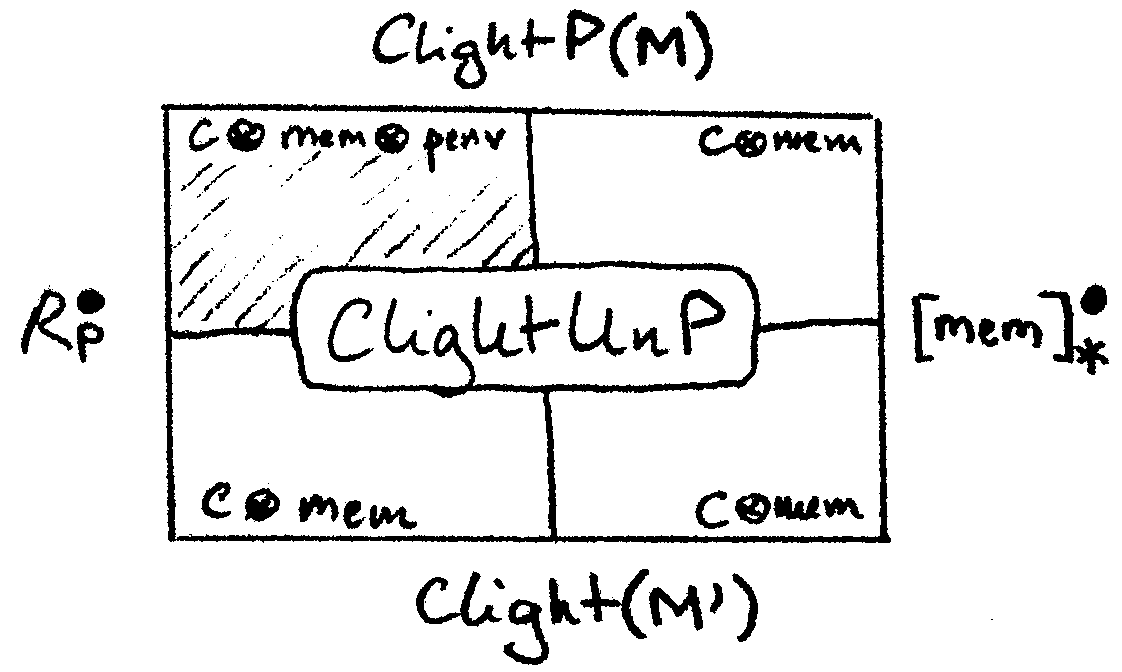
\includegraphics[scale=0.1]{draftfig/unclight}} }
  \,,
  \quad
  \text{where}
  \quad
  R_\kw{P}^\bullet =
    \vcenter{ \hbox{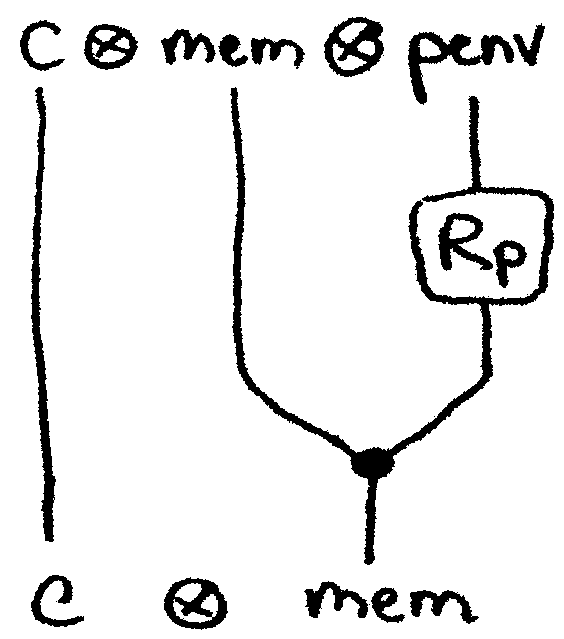
\includegraphics[scale=0.09]{draftfig/unclight-ccb}} }
    \,,
  \qquad
  [\kw{mem}]_*^\bullet =
    \vcenter{ \hbox{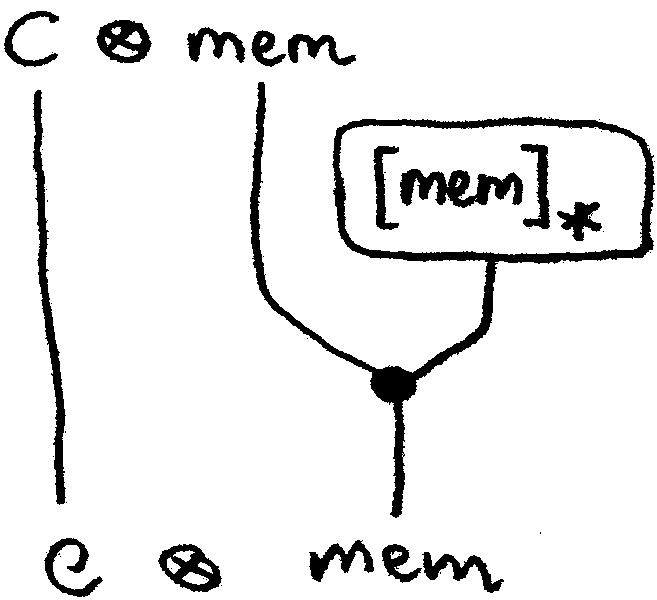
\includegraphics[scale=0.09]{draftfig/unclight-cca}} }
    \,.
\]
The Clight program
stores formerly private variables in the main memory.
For incoming calls,
the private environment is refined
into a memory share according to a relation $R_\kw{P}$,
and is then merged with the main memory.
For outgoing calls,
the private environment is not included in the source question,
but the variables are still stored in the target memory.
The use of $[\kw{mem}]_*^\bullet$
requires the callee to return
this region of the memory unchanged.

\subsection{Encapsulating Private Environments}

In order to give the semantics
a more tractable type,
we can encapsulate the private environment:
\[
  \kw{ClightP} \langle M \rangle :=
    (C \mathbin@ \kw{mem} \mathbin@ \langle p_0 \rangle_*) \odot
    \kw{ClightP}(M)
    :
    \mathcal{C} \mathbin@ \kw{mem} \twoheadrightarrow
    \mathcal{C} \mathbin@ \kw{mem}
\]
Here $p_0 := \kw{init\_penv}(M)$ is the initial private environment for $M$.
The facilities discussed in \S\ref{sec:overview:encap}
can then be used to
derive a correctness property
stated in terms of the encapsulated semantics:
\[
  \draftfig{0.08}{encap-clightunp}
\]
Here, $m_0 := \kw{init\_mem} \big(M'_\kw{priv}\big)$
is the initial memory fragment associated with
the global variable definitions introduced in $M'$
in order to implement the private variables of $M$.
Note that private environments
no longer appear in the type of the ClightP semantics
or in the correctness property.

\subsection{Composition}

One challenge is that the correctness property depicted above
is not compositional,
because the incoming and outgoing simulation conventions are different:
\[
    \kw{ClightP}\langle M \rangle
      \le_{\mathcal{C} \otimes \langle m_0 \rangle_*^\bullet
           \twoheadrightarrow
           \mathcal{C} \otimes [\kw{mem}]_*^\bullet}
      \kw{Clight}(M')
\]
Two ClightP modules
$
  \kw{ClightP} \langle M_1 \rangle \odot \kw{ClightP}\langle M_2 \rangle
$
can be composed,
but the associated $\kw{ClightUnP}$ correctness properties
do not directly compose alongside them.
We will use the following strategy:
\[
  \draftfig{0.09}{clightp-comp}
\]
First,
we will establish self-simulation properties
for $\kw{ClightP}$ (1) and $\kw{Clight}$ (2)
which show that they are compatible with
the simulation conventions $\langle m \rangle_*^\bullet$
and $[\kw{mem}]_*^\bullet$.
These properties follow mainly from the frame rule
of our memory separation primitives.
Second,
we show that the incoming (3) and outgoing (4)
simulation conventions compose with themselves.

First,
the property
$
  \kw{Clight}(M)
  \le_{\langle m \rangle_*^\bullet \twoheadrightarrow \langle m \rangle_*^\bullet}
  \kw{Clight}(M)
$,
stems from the fact that
\[
L \odot (A \mathbin@ \langle u \rangle) = L \mathbin@ \langle u \rangle =
 (B \mathbin@ \langle u \rangle) \odot (L \mathbin@  U)
  \quad\text{for any}  \quad L : A \twoheadrightarrow B
  \,.
\]
This can be combined with the frame rule and properties of $\langle m_0 \rangle_*$ to show:
\[
  \draftfig{0.08}{spinwheel}
\]
A similar argument can be used to show
the analogous property of ClightP.

Second,
the self-composition of the simulation conventions involved
follows mostly from properties of the partial commutative monoid.

%}}}

\section{Encapsulated State} \label{sec:encap} %{{{

% Preamble {{{
We now construct the version of our model
which allows state components to be encapsulated.
The underlying transition systems are unchanged,
and encapsulated state
is communicated from one activation to the next
in the same way global state would be.
However,
marking state as encapsulated
removes it from a component's type,
and prevents the environment from accessing it.
%}}}

\subsection{Components} %{{{

The compositional treatment of state
presented in \S\ref{sec:scomp}
allows a component $L_1 : B \rightarrow C \in \mathbf{TS}$
to interact with %a component
$L_2 : A \rightarrow B \mathbin@ U$
as the composite $(L_1 \mathbin@ U) \odot L_2$.
This guarantees that
$L_1$ will not interfere with the state in $U$.
Our approach to state encapsulation
is to force the environment to
interact with components in this manner.
In the extended model,
a component $L : A \rightarrow B \in \mathbf{TS}^\dagger$
is defined using an underlying transition system
of type $A \rightarrow B \mathbin@ U$
with
an additional state component $U \in \mathbf{Bij}$.

\begin{definition} \label{def:slts}
Consider a category $\mathbf{C}$
equipped with a functor
${\star} : \mathbf{C} \times \mathbf{Bij} \rightarrow \mathbf{C}$
and a family of isomorphisms
$
  \alpha_{A,U,V} : A \star (U \times V) \cong A \star U \star V
$.
We define a category $\mathbf{C}^\dagger$
with the same objects,
where morphism take the form
$(u \in U \mid L) : A \rightarrow B \in \mathbf{C}^\dagger$
and consist of:
\begin{itemize}
  \item a set of states $U$ with a distinguished initial state $u \in U$;
  \item a morphism $L : A \rightarrow B \star U \in \mathbf{C}$
    of the underlying category.
\end{itemize}
Composition in $\mathbf{C}^\dagger$ is defined as:
\[
  (u \in U \mid L_1) \,\circ\, (v \in V \mid L_2) \::=\:
  \big( (u, v) \in U \times V \mid
        \alpha^{-1} \circ (L_1 \star V) \circ L_2 \big)
\]
An embedding of $\mathbf{C}$ into $\mathbf{C}^\dagger$
is defined by $(* \in \mathbbm{1} \mid {-})$.
\end{definition}

The construction above can be applied both to
the active components in $\mathbf{TS}$ (with ${\star} := {\mathbin@}$) and
the passive components in $\mathbf{Bij}$ (with ${\star} := {\otimes}$).
The first time a component
$(u \in U \mid L) : A \rightarrow B \in \mathbf{TS}^\dagger$
is activated by a question $q \in B^\que$,
%the state $u$ is adjoined to $q$ and
the transition system $L$ is initialized using %the question
$q@u \in (B \mathbin@ U)^\que$.
When $L$ terminates with an answer $r@u' \in (B \mathbin@ U)^\ans$,
the component passes $r \in B^\ans$ on to the environment and
the new state $u'$ is set aside to be used with the next activation.

In addition to composition,
the functor ${\star} : \mathbf{C} \times \mathbf{Bij} \rightarrow \mathbf{C}$
can also be extended to
${\star} : \mathbf{C}^\dagger \times \mathbf{Bij}^\dagger \rightarrow \mathbf{C}^\dagger$.
This can be shown using string diagrams of the following form:
\[
  \draftfig{0.1}{encap-comp}
  \qquad\qquad
  \draftfig{0.08}{encap-tens}
\]
where the beads on the left-hand side
represent the encapsulated state components.
This representation stems from the fact that
any morphism in $\mathbf{C}^\dagger$
can be defined using the embedded morphisms of $\mathbf{C}$
together with the following state encapsulation primitive:
\[
  \langle u \in U \rangle : U \rightarrow \mathbbm{1} \in \mathbf{Bij}^\dagger
  \qquad \qquad
  \langle u \in U \rangle  :=  (u \in U \mid \kw{id}_U)
    = \quad u \circ \!\!-
\]

%Once private state has been encapsulated,
%in principle it can only be observed by the environment
%through the way the transition system responds
%to successive queries.
%In particular,
%constructions on stateful components
%should preserve the following notion of equivalence.
%
%\begin{definition}[Simple Simulation] \label{def:ssim}
%We will say that $\Sigma_1 : A \rightarrow B$
%is refined by $\Sigma_2 : A \rightarrow B$
%and write $\Sigma_1 \preceq \Sigma_2$
%when there exists a relation $R \subseteq K_1 \times K_2$
%such that:
%\begin{itemize}
%  \item the initial states $\intl{k}_1, \intl{k}_2$ are related by $R$;
%  \item the transition systems satisfy
%    $L_1 \le_{\kw{id}_A \twoheadrightarrow B@R} L_2$.
%\end{itemize}
%We write $\Sigma_1 \equiv \Sigma_2$ when
%$\Sigma_1 \preceq \Sigma_2$ and
%$\Sigma_2 \preceq \Sigma_1$.
%\end{definition}

%}}}

%\subsection{Composition} %{{{
%
%The composite $\Sigma_1 \circ \Sigma_2$
%uses states of type $K_1 \times K_2$.
%Each side of the pair is updated
%when the corresponding component is active.
%Incoming questions in $C$ are routed to $L_1 : B \twoheadrightarrow C@K_1$,
%which we lift to pass through an additional state component of type $K_2$.
%Outgoing questions of $L_1$ in $B$ can then be routed to $L_2$,
%as depicted in the following diagram:
%\[
%  \begin{tikzpicture}[yscale=0.5]
%    \draw (0,2) node[left] {$K_2$} -- (2,2) .. controls +(0.5,0) and +(-0.5,0) .. (3,1);
%    \draw (0,1) node[left] {$K_1$} -- (1,1);
%    \draw (0,0) node[left] {$C$} -- (1,0);
%    \draw (2,0) -- node[below] {$B$} (3,0);
%    \draw (4,0) -- (5,0) node[right] {$A$};
%    \draw (1,1.5) rectangle node {$L_1$} (2,-0.5);
%    \draw (3,1.5) rectangle node {$L_2$} (4,-0.5);
%  \end{tikzpicture}
%\]
%Formally,
%composition is defined as follows.
%
%\begin{definition}[Composition] \label{def:slcomp}
%Given two stateful components
%$\Sigma_1 = (K_1 \mid L_1) : B \rightarrow C$ and
%$\Sigma_2 = (K_2 \mid L_2) : A \rightarrow B$,
%we define their composition
%$\Sigma_1 \circ \Sigma_2 : A \rightarrow C$
%in the following way:
%\[
%  \Sigma_1 \circ \Sigma_2 :=
%    ( K_1 \times K_2 \mid L_1@K_2 \odot L_2 )
%\]
%Note that this formulation
%implicitly uses the isomorphism
%\[
%  L_1@K_2 : B@K_2 \twoheadrightarrow (C@K_1)@K_2 \cong C@(K_1 \times K_2)
%  \,.
%\]
%\end{definition}
%
%
%
%
%\begin{lemma}
%  This is compatible with:
%  \begin{itemize}
%    \item simple simulations;
%    \item lifting hence associativity is preserved.
%  \end{itemize}
%
%\end{lemma}
%
%%}}}

%\subsection{Combining Hidden and Explicit State} %{{{
%
%It is possible for a stateful component
%to hide only part of the explicit state
%used by the underlying transition system.
%For example,
%in a transition system
%$L : A \rightarrow B@(K \times U) \cong B@U@K$,
%we may choose to hide only $K$,
%to obtain a stateful component
%$\Sigma = (K \mid L) : A \rightarrow B@U$
%which still exchanges explicit state of type $U$
%with the environment.
%This makes it possible to construct
%complex stateful components incrementally
%from simpler, stateless parts,
%by first promoting them using $\&$,
%then hiding state in a step-by-step fashion
%using $\kw{fbk}$.
%
%In addition,
%stateful components can be lifted
%to pass through explicit state.
%
%\begin{definition} \label{def:slift}
%The stateful component $\Sigma = (K \mid L) : A \rightarrow B$
%can be lifted to \[ \Sigma@U := (K \mid L@U) : A@U \rightarrow B@U \,. \]
%Note that this relies on the isomorphism
%\[
%  L@U : A@U \twoheadrightarrow (B@K)@U \cong (B@U)@K
%  \,.
%\]
%\end{definition}
%
%The following properties
%relate the promotion operator $\&$,
%the composition operators $\odot$ and $\circ$,
%and the hiding operator $\kw{fbk}$.
%
%\begin{lemma}
%  For $L_1 : B \twoheadrightarrow C@K_1$ and
%  $L_2 : A \twoheadrightarrow B@K_2$,
%  the following property holds:
%  \[
%    \&(L_1@K_2) \circ \&L_2 \equiv \&(L_1@K_2 \odot L_2)
%    \,.
%  \]
%  In addition, for $\Sigma_1 : B \rightarrow C@U_1$
%  and $\Sigma_2 : A \rightarrow B@U_2$,
%  the following property holds:
%  \[
%    \kw{fbk}_{U_1}(\Sigma_1) \circ \kw{fbk}_{U_2}(\Sigma_2) \equiv
%    \kw{fbk}_{U_1 \times U_2}(\Sigma_1@U_2 \circ \Sigma_2)
%    \,.
%  \]
%\end{lemma}
%
%%}}}

\subsection{Simulations} %{{{

We must now extend the double category structure of $\mathbf{TSC}$
to the encapsulated state model.
The same notion of simulation convention can be reused as-is.
In addition,
the simulation property
$L^\sharp \le_{\mathbf{R} \rightarrow \mathbf{S}} L^\flat \in \mathbf{TSC}^\dagger$
can be defined using a simulation
in the original model $\mathbf{TSC}$
between the underlying transition systems.
However,
to take into account the components' encapsulated states,
we must first incorporate those states into
the incoming simulation convention $\mathbf{S}$.
To this end,
we will use the elementary simulation conventions
$\langle u \rangle^*$ and $\langle u \rangle_*$
mentioned in \S\ref{sec:overview:encap}.

\begin{definition}
For $u \in U$,
the simulation conventions
$\langle u \rangle^*$ and
$\langle u \rangle^*$ are defined as:
\[
  \langle u \rangle^* :=
    \big\langle U,\, u,\, \top,\, {=},\, \Gamma_U,\, \Gamma_U \big\rangle
    : U \leftrightarrow \mathbf{I}
  \qquad \qquad
  \langle u \rangle^* :=
    \big\langle U,\, u,\, \top,\, {=},\, \Gamma_U^\kw{op},\, \Gamma_U^\kw{op} \big\rangle
    : \mathbf{I} \leftrightarrow U
\]
where $\Gamma_U \in \mathcal{R}(U, \mathbbm{1})$
is the smallest Kripke relation containing $u \Vdash u \mathrel{\Gamma_U} *$ for all $u \in U$.
\end{definition}

These elementary simulation conventions
internalize a state component of type $U$ in their Kripke worlds,
and express the guarantees provided by the environment
for encapsulated state:
on the first call, the source (resp. target) component
must be passed the initial state $u \in U$.
It may then modify the state,
performing a callee world transition
in $\langle u \rangle^*$ (resp. $\langle u \rangle_*$).
However,
between successive calls,
the caller may not update the world.
With the ability to express these constraints,
we can define our notion of simulation
for components with encapsulated states.

\begin{definition} \label{def:ssim} %{{{
Simulations of components with encapsulated state are defined by
\[
  (u \in U \mid L^\sharp)
  \le_{\mathbf{R} \rightarrow \mathbf{S}}
  (v \in V \mid L^\flat)
  \in \mathbf{TSC}^\dagger
  \quad:\Leftrightarrow\quad
  L^\sharp
  \le_{\mathbf{R} \rightarrow
       \mathbf{S} \otimes (\langle u \rangle^* \mathbin; \langle v \rangle_*)}
  L^\flat
  \in
  \mathbf{TSC}
  \,.
\]
\end{definition}
%}}}

As in $\mathbf{TSC}$,
simulations in $\mathbf{TSC}^\dagger$ compose
horizontally and vertically.

\begin{theorem} %{{{
Language interfaces, encapsulated transition systems, simulation conventions
and simulations in the sense of Def.~\ref{def:ssim}
constitute a double category $\mathbf{TSC}^\dagger$.
There is an embedding double functor $\mathbf{TSC} \hookrightarrow \mathbf{TSC}^\dagger$
which preserves the compositional structure of $\mathbin@$ and $\otimes$.
\end{theorem}
%}}}

%}}}

%}}}

\section{Related Work} %{{{

\subsection{CompCert-based Vertification Frameworks}

CompCert \cite{compcert}
is the first certified C compiler offering industrial-grade performance.
As a result,
there has long been interest in extending the compiler
to offer verification frameworks
with formal guarantees going all the way to assembly code.
For example, VST \cite{vst}
provides a separation logic for Clight
whose soundness proof interfaces with CompCert's correctness proof.

\paragraph{Compositional Semantics}

Compositional semantics were introduced by
Compositional CompCert \cite{compcompcert}
in part to support the verification of
programs with multiple translation units,
potentially written in different languages,
but used a fixed language interface and simulation convention.
CompCertM \cite{compcertm} refined this approach
with a better model of the interaction between
C and assembly programs,
and more flexibility in simulation conventions,
making it possible for example to introduce of module-local state
by expressing constraints on the environment.
However, neither Compositional CompCert nor CompCertM
support data abstraction or state encapsulation
of the kinds we have presented,
and the general notions of
language interface and simulation convention
were first introduced in CompCertO.
We refer interested readers to \citet{compcerto}
for a detailed comparison between Compositional CompCert,
CompCertM and CompCertO.

Interaction trees \cite{itree,itrees} provide
another framework for compositional semantics
formalized in the Coq proof assistant
which presents similarities with our own,
though their interface with CompCert is less comprehensive.

\paragraph{Certified Abstraction Layers}

Data abstraction in a form closer to our own
is present in certified abstraction layers (CAL),
originally implemented by CompCertX \cite{popl15}
to verify the certified operating CertiKOS.
The semantic model of CompCertX can be summarized as
\[
  \forall D \in \mathbf{Set}
  \: \mathbin. \:
  L^\flat :
    \top \twoheadrightarrow
    \mathcal{C} \mathbin@ \kw{mem} \mathbin@ D^\flat
  \: \vdash \:
  \kw{Clight}_{L^\flat}[M] :
    \top \twoheadrightarrow
    \mathcal{C} \mathbin@ \kw{mem} \mathbin@ D^\flat
  \,.
\]
Here $L^\flat$ is an \emph{underlay interface}.
The goal is to implement an \emph{overlay}
$
  L^\sharp \le_{\top \twoheadrightarrow \mathcal{C}@R}
    \kw{Clight}_{L^\flat}[M]
$,
in a way which allows to abstraction relation
$R \subseteq (\kw{mem} \times L^\sharp) \times (\kw{mem} \times L^\flat)$
to refine and augment the abstract data component.
Layers verified in this way can then be combined sequentially.

Subsequent work has extended CAL to support concurrency \cite{ccal}.
The original model is tied to the CompCert semantics and
further work explores more abstract versions \cite{rbgs-cal,popl22}.
In particular a version of the $\mathbin@$ construction appears in \citet{rbgs-cal}.
However, these more abstract frameworks
have not been implemented.

\subsection{Categorical Structures}

To our knowledge,
the work described in this paper
constitutes the first formal and explicit use of
double categories in the context of compositional verification,
although the approach was initially suggested in \citet{compcerto}.
String diagrams for double categories,
which use for simulation proofs,
were developed and shown to be sound in \citet{dcsd}.
Monoidal categories and their string diagrams
are much more ubiquitous---a good introduction is provided by \citet{rosetta}.

The construction $\mathbf{C}^\dagger$ which we used in \S\ref{sec:encap}
bears some resemblance and was inspired by
the \emph{free category with feedback} construction \cite{feedback,caots}.
Indeed,
traced monoidal categories
could provide a basis for encapsulation
in a version of our framework supporting reentrancy and mutual recursion,
as in interaction trees.
The present version
based on an elementary encapsulation primitive $\langle u \rangle$
is simpler but less powerful.

%\paragraph{Accessibility Condition}
%
%The $\sqsubseteq_{\kw{prv}}$ is similar to $\leadsto_{\bar{A}B}$
%while $\sqsubseteq$ is similar to $\leadsto_{AB}$. Or maybe not...
%
%\paragraph{Module Static Variables}
%
%\citet{compcertm} presents CompCertM,
%which supports module-static variables
%and reasoning about mutually recursive programs.
%The difficulty is to capture the effects that external calls may have on
%those variables through reentrant calls.
%\citet{compcertm} further generalizes the memory injection
%to include a notion of module-local invariants
%to enable reasoning on such variables.
%We could generalize the simulation convention in a similar manner
%to achieve the same reasoning power.
%However, for the purpose of revamping the CAL framework,
%mutual recursion is considered unnecessary
%so we keep things simple.

%}}}

\section{Conclusion} %{{{

It is argued in \citet{compcerto}
that the use of compositional semantics
and the formalization of abstraction
provided by simulation conventions
are important steps towards
the construction of large-scale systems certified end-to-end.
We have sought to take a further step in this direction
by incorporating data abstraction and
compositional state encapsulation
into CompCertO's framework.

We believe in particular that
the underlying algebraic structures that we have uncovered
in this process
provide an elegant structure
with applications beyond the present work,
and may constitute an important facet of
future certified systems engineering work.

%}}}

\bibliography{../references}

\appendix

\newpage

\section{Memory Separation in CompCert} \label{sec:sep} %{{{

The constructions we have introduced so far
make it possible to manage and encapsulate persistent state
in the context of CompCertO,
with certified abstraction layers
as one key application.
The global memory state used in the semantics of CompCert languages
can then be regarded as one possible kind of state among others,
and replaced in specifications by more abstract data representations.

Unfortunately,
because of the monolithic nature of CompCert's memory,
abstracting only part of it is challenging
and yields complex simulation conventions.
In Example~\ref{ex:rbcorrect},
the abstraction relation had to involve
not only the whole target memory state,
but also the residual source memory state
not subject to abstraction,
and used complex properties to express their relationships.
In other words,
instead of focusing on the particular fragment of the memory
which we seek to abstract away,
we are to forced to characterize the effect of partial abstraction
on the context as well,
even though the remaining areas of the memory
are not meaningfully involved in the task at hand.

In this section,
we use techniques from separation logic
to address this problem.
We propose to equip the CompCert memory model
with a structure akin to separation algebra \cite{something-for-sa}
and incorporate the resulting construction
within the framework of simulation conventions,
CompCert Kripke logical relations,
and state encapsulation.

\subsection{The CompCert Memory Model}

In essence,
a CompCert memory state
assign to each possible memory address $i \in \kw{block} \times \mathbb{Z}$:
\begin{itemize}
  \item a permission level $p \in \kw{option}\,\kw{perm}$;
  \item a memory value $v \in \kw{memval}$.
\end{itemize}
In addition,
a memory state contains a $\kw{nextblock}$ counter
which keeps track of the next block identifier to be allocated.
We discuss these various components in more detail below.

\subsubsection{Memory Addresses}

The CompCert memory is divided in a number of \emph{blocks}.
As new blocks are allocated,
they are assigned a positive identifier $b \in \mathbb{N}_*$
in sequential order.
As mentioned above,
the $\kw{nextblock}$ counter within each memory state
keeps track of the smallest unallocated block identifier.
When a new block identifier is needed,
$\kw{nextblock}$ is incremented and its previous value
is used for the new block.

Memory blocks represent independent address spaces.
Within each block,
a byte can be addressed using an offset $o \in \mathbb{Z}$.
When a new block is allocated,
a range of addresses $[\mathit{lo}, \mathit{hi})$ must be provided;
this range determines which addresses within the block are valid.
However,
rather than storing the range directly within the memory state,
the allocation operation uses it to assign initial permissions
for each address within the new block.

\subsubsection{Permissions}

Each memory address within a memory state
is assigned a permission level among the following:
\[
  p \in \kw{option}\,\kw{perm} ::=
    \bot \mid
    \kw{nonempty} \mid
    \kw{readable} \mid
    \kw{writable} \mid
    \kw{freeable}
\]
The permissions are listed above in increasing order,
so that for example the permission level $\kw{writable}$ 
represents the set of permissions
$\{ \kw{nonempty}, \kw{readable}, \kw{writable} \}$.
Permissions play an important role
in the memory separation relation we define.

When a block is first allocated,
addresses within the provided range
are assigned the permission level $\kw{freeable}$;
all remaining addresses are assigned
empty permissions $\bot$.
Further memory operations may then decrease the permission level,
but can never increase it.
Memory operations which access a particular address
will first check that this address has sufficient permissions,
and fail if that is not the case.

\subsubsection{Memory Values}

Each memory value represents the contents of exactly one byte of memory.
It may be stored as a concrete byte,
or may be identified as a particular one-byte fragment
within a larger, more abstract value
(for instance, the third byte of a given pointer).

The exact representation of memory values
is not essential to the work discussed in this section.
Therefore
we will not discuss the specifics further,
but refer the interested reader to \citet{compcertmmv2}
for more background on this topic.

\subsubsection{Memory Transformations}

The compilation passes of CompCert
often transform the structure of the memory state:
multiple blocks can merged into one;
new blocks may be introduced in the target memory
and blocks may be dropped from the source memory.
To express these transformations,
CompCert introduces \emph{memory extensions} and \emph{memory injections}
as possible relations between source- and target-level memory states.

In CompCertO,
these memory transformations are generalized and consolidated
into a notion of \emph{CompCert Kripke Logical Relations} (CLKRs),
which play an important role in defining simulation conventions.
The underlying idea is that
if two memory states are related by a CKLR,
then memory operations which succeed at the source level
should also succeed on at the target level,
and their outcomes should in turn be related
by the CKLR.

Unfortunately,
these memory transformations are difficult to use
to express the relationships between
different \emph{fragments} of a single memory state.
The notion of \emph{separation relation} introduced below
seeks to fill this gap.

\subsection{Separation Relations} %{{{

To express memory separation in CompCert,
and define a \emph{join} relation
$J \subseteq (\kw{mem} \times \kw{mem}) \times \kw{mem}$.
We will write $J(m_1, m_2, m)$ as:
\[
  m_1 \bullet m_2 \equiv m
  \,,
\]
understood to mean that
the memory states $m_1$ and $m_2$
can be merged into $m$.
This relation satisfies the properties listed in Fig.~\ref{fig:sepalg}
and defines a separation algebra in the sense of \citet{freshlook}.

\begin{figure}
  \begin{gather*}
    m_1 \bullet m_2 \equiv m \:\wedge\:
      m_1 \bullet m_2 \equiv m' \:\Rightarrow\:
      m = m'
      \\
    m_1 \bullet m_2 \equiv m \:\wedge\:
      m_1' \bullet m_2 \equiv m \:\Rightarrow\:
      m_1 = m_1'
      \text{ XXX}
      \\
    m_1 \bullet m_2 \equiv m \:\Rightarrow\:
      m_2 \bullet m_1 \equiv m
      \\
    m_1 \bullet m_2 \equiv m_{12} \:\wedge\:
      m_{12} \bullet m_3 \equiv m \:\Rightarrow\:
      \exists m_{23} \mathrel.
      m_2 \bullet m_3 \equiv m_{23} \:\wedge\:
      m_1 \bullet m_{23} \equiv m
      \\
    m \bullet \kw{empty} \equiv m
  \end{gather*}
  \caption{Properties of separation algebras
    in relational form. See also \citet{freshlook}.}
  \label{fig:sepalg}
\end{figure}

In addition to these structural properties,
the join relation must be compatible
with CompCert's memory operations.
If an operation which reads from the memory succeeds on a fragment,
it should succeed with the same result on a larger memory state:
\[
  \begin{prooftree}
    \hypo{\kw{op}(m_1) = \kw{Some}\,v}
    \hypo{m_1 \bullet m_2 \equiv m}
    \infer2{\kw{op}(m) = \kw{Some}\,v}
  \end{prooftree}
\]
Likewise,
operations which updates the memory
should be insensitive to additional fragments:
\[
  \begin{prooftree}
    \hypo{\kw{op}(m_1) = \kw{Some}\,m_1'}
    \hypo{m_1 \bullet m_2 \equiv m}
    \infer2{\exists m' \mathrel.
      m_1' \bullet m_2 \equiv m' \wedge
      \kw{op}(m) = \kw{Some}\,m'}
  \end{prooftree}
\]

Together,
these properties allow us to derive
versions of the \emph{frame rule}
for CompCert languages:
if a program can successfully execute on $m_1$ alone
to yield a new memory fragment $m_1'$,
then executing it on a larger memory state
$m_1 \bullet m_2$ will succeed as well,
and yield a memory state $m_1' \bullet m_2$
where the irrelevant portion $m_2$
has not been modified.

Moreover,
executions which affect disjoint parts of the memory
can be considered independently.
Specifically, from the rules above
we can derive the property:
\[
  \begin{prooftree}
    \hypo{\kw{op}_1(m_1) = \kw{Some}\,m_1'}
    \hypo{\kw{op}_2(m_2) = \kw{Some}\,m_2'}
    \hypo{m_1 \bullet m_2 \equiv m}
    \infer3{\exists m' \mathrel.
      \kw{op}_1(\kw{op}_2(m)) =
	%\kw{op}_2(\kw{op}_1(m)) =
	m' \:\wedge\:
      m_1' \bullet m_2' \equiv m'}
  \end{prooftree}
\]
As in separation logic,
this facilitates reasoning
about program components
which affect the memory state in independent ways.

Below we explain how a separation relation can be defined
for the CompCert memory model.

\subsubsection{Memory Contents}

A CompCert memory state essentially defines a map of type
\[
  \kw{ptr} \rightarrow \kw{option}\,\kw{perm} \times \kw{memval} \,,
\]
which assigns to every possible address
a permission level and a memory value.
Figure~\ref{fig:sepdef}
shows the definition of a simple separation relation
for the contents of individual memory cells.
This relation can then be extended to the whole map
in the obvious way.

\begin{figure}
  \begin{subfigure}{0.45\textwidth}
    \centering
    \fbox{$J_\kw{contents}$}
    \begin{gather*}
      (p, v) \in \kw{option}\ \kw{perm} \times \kw{memval} \\[1ex]
      (\bot, \kw{undef}) \bullet (p, v) \equiv (p, v) \\
      (p, v) \bullet (\bot, \kw{undef}) \equiv (p, v)
    \end{gather*}
    \subcaption{Memory contents}
    \label{fig:sepdef:contents}
  \end{subfigure}
  \begin{subfigure}{0.45\textwidth}
    \centering
    \fbox{$J_\kw{nextblock}$}
    \begin{gather*}
      (\mathit{nb}, a) \in \kw{block} \times \kw{bool}
      \\[1ex]
     {\begin{prooftree}
	\hypo{\mathrm{max}(\mathit{nb}_1, \mathit{nb}_2) = \mathit{nb}}
	\hypo{\lnot (a_1 \wedge a_2)}
	\infer2{(\mathit{nb}_1, a_1) \bullet (\mathit{nb}_2, a_2) \equiv
	  (\mathit{nb},\, a_1 \mathbin\vee a_2)}
      \end{prooftree}}
    \end{gather*}
    \subcaption{Fresh blocks}
    \label{fig:sepdef:fresh}
  \end{subfigure}
  \caption{%
    Basic ingredients for separation algebras
    of the CompCert memory model.}
  \label{fig:sepdef}
\end{figure}

\subsubsection{Block Validity}

A more challenging issue is the treatment of $\kw{nextblock}$.
When a memory state $m$ is separated into $m_1 \bullet m_2 \equiv m$,
the fragments $m_1$ and $m_2$ will share a common view of the address space.
However,
they each carry their own copy of the $\kw{nextblock}$ counter.
As a result,
performing independent allocations in each fragment
will break the separation property,
because the new blocks will be assigned conflicting names.

As a starting point,
we solve this problem by
making sure that new blocks
can only be allocated in one of the fragments.
In addition to the $\kw{nextblock}$ counter,
memory states carry a boolean flag
indicating whether allocations are permitted.
When memory fragments are joined,
this flag can only be set in one of the fragments.
Figure~\ref{fig:sepdef:fresh}
shows the corresponding separation algebra
for the $\kw{nextblock}$ counter.

%}}}

\subsection{Frame rule} %{{{

The compatibility of memory operations with our separation algebras
can be used to show that
more complex ways to manipulate memory states
enjoy similar properties.
Ultimately this allows us to derive
a kind of \emph{frame rule} for the Clight semantics.
We can state this informally as follows:
\[
  \begin{prooftree}
    \hypo{\Clight(p) : m_1 \leadsto m_2}
    \infer1{\Clight(p) : m_1 \bullet m \leadsto m_2 \bullet m}
  \end{prooftree}
\]
In other words,
if the program $p$ safely acts on a memory state $m_1$
to transform it into a memory state $m_2$,
then we can frame a memory fragment $m$ onto $m_1$
and expect the program to leave that fragment intact.
Intuitively, this holds because
if $p$ ever needed or affected any of the memory present
in fragment $m$,
it would have gone wrong on $m_1$ alone.

To formalize this property in the context of CompCertO,
we can promote the memory separation relation
to a simulation convention:
\[
  \forall A \:.\quad
  A@{\bullet} : A@(\kw{mem} \times \kw{mem}) \leftrightarrow A@\kw{mem}
\]
We will then compare the ``source''-level semantics
\[
  \Clight(p)@\kw{mem} :
    \mathcal{C}@(\kw{mem} \times \kw{mem}) \twoheadrightarrow
    \mathcal{C}@(\kw{mem} \times \kw{mem})
  \,,
\]
which acts on one of the memory fragments
but leaves the other one unchanged,
to the concrete semantics of $p$ acting on the total memory state:
\[
  \Clight(p) : \mathcal{C}@\kw{mem} \leftrightarrow \mathcal{C}@\kw{mem}
  \,.
\]
This yields the following property.

\begin{lemma}[Frame rule for Clight]
\[
  \Clight(p)@\kw{mem}
  \le_{\mathcal{C}@{\bullet} \twoheadrightarrow \mathcal{C}@{\bullet}}
  \Clight(p)
\]
\end{lemma}

%}}}

%}}}

\end{document}
\endinput

\newpage

\begin{figure}[h] %{{{
  \textbf{Notations}
  \\[1em]
  \begin{tabular}{llcllc}
    Basic component & Def.~\ref{def:lts} &
    $L : A \twoheadrightarrow B$ &
    Stateful component & Def.~\ref{def:slts} &
    $\Sigma : A \rightarrow B$
    \\
    Basic convention & Def.~\ref{def:simconv} &
    $\mathbb{R} : A^\sharp \Leftrightarrow A^\flat$ &
    Stateful convention & Def.~\ref{def:sconv} &
    $\mathbf{R} : A^\sharp \leftrightarrow A^\flat$
    \\
    Basic simulation & Def.~\ref{def:sim} &
    $L^\sharp \le_{\mathbb{R}_A \twoheadrightarrow \mathbb{R}_B} L^\flat$ &
    Stateful simulation & Def.~\ref{def:ssim} &
    $\Sigma^\sharp \preceq_{\mathbf{R}_A \rightarrow \mathbf{R}_B} \Sigma^\flat$
  \end{tabular}
  \\[1em]
  \textbf{Layered composition}
  \\[1em]
  \begin{tabular}{cc@{\qquad}cc}
    Def.~\ref{def:lcomp} &
  {$\begin{prooftree}
      \hypo{L_1 : B \twoheadrightarrow C}
      \hypo{L_2 : A \twoheadrightarrow B}
      \infer2{L_1 \odot L_2 : A \twoheadrightarrow C}
    \end{prooftree}$}
    &
    Def.~\ref{def:slcomp} &
  {$\begin{prooftree}
      \hypo{\Sigma_1 : B \rightarrow C}
      \hypo{\Sigma_2 : A \rightarrow B}
      \infer2{\Sigma_1 \circ \Sigma_2 : A \rightarrow C}
    \end{prooftree}$}
    \vspace{1em} \\
    Thm.~\ref{thm:lcompsim} &
  {$\begin{prooftree}
      \hypo{L_1^\sharp
            \le_{\mathbb{R}_B \twoheadrightarrow \mathbb{R}_C}
            L_1^\flat}
      \hypo{L_2^\sharp
            \le_{\mathbb{R}_A \twoheadrightarrow \mathbb{R}_B}
            L_2^\flat}
      \infer2{L_1^\sharp \odot L_2^\sharp
            \le_{\mathbb{R}_A \twoheadrightarrow \mathbb{R}_C}
            L_1^\flat \odot L_1^\flat}
    \end{prooftree}$} &
    Thm.~\ref{thm:slcompsim} &
  {$\begin{prooftree}
      \hypo{\Sigma_1^\sharp
            \preceq_{\mathbf{R}_B \rightarrow \mathbf{R}_C}
            \Sigma_1^\flat}
      \hypo{\Sigma_2^\sharp
            \preceq_{\mathbf{R}_A \rightarrow \mathbf{R}_B}
            \Sigma_2^\flat}
      \infer2{\Sigma_1^\sharp \circ \Sigma_2^\sharp
            \preceq_{\mathbf{R}_A \rightarrow \mathbf{R}_C}
            \Sigma_1^\flat \circ \Sigma_1^\flat}
    \end{prooftree}$}
  \end{tabular}
  \\[1em]
  \textbf{Vertical composition}
  \\[1em]
  \begin{tabular}{cc@{\qquad}cc}
    Def.~\ref{def:ccomp} & {$
    \begin{prooftree}
      \hypo{\mathbb{R} : A^\sharp \Leftrightarrow A^\natural}
      \hypo{\mathbf{S} : A^\natural \Leftrightarrow A^\flat}
      \infer2{\mathbb{R} \cdot \mathbf{S} : A^\sharp \Leftrightarrow A^\flat}
    \end{prooftree}
    $} &
    Def.~\ref{def:sccomp} & {$
    \begin{prooftree}
      \hypo{\mathbf{R} : A^\sharp \leftrightarrow A^\natural}
      \hypo{\mathbf{S} : A^\natural \leftrightarrow A^\flat}
      \infer2{\mathbf{R} \mathbin; \mathbf{S} : A^\sharp \leftrightarrow A^\flat}
    \end{prooftree}
    $}
    \vspace{1em} \\
    Thm.~\ref{thm:vcomp} & {$
    \begin{prooftree}
      \hypo{L^\sharp
        \le_{\mathbb{R}_A \twoheadrightarrow \mathbb{R}_B}
        L^\natural}
      \hypo{L^\natural
        \le_{\mathbf{S}_A \twoheadrightarrow \mathbf{S}_B}
        L^\flat}
      \infer2{L^\sharp
        \le_{\mathbb{R}_A \cdot \mathbf{S}_A \twoheadrightarrow
             \mathbb{R}_B \cdot \mathbf{S}_B}
        L^\flat}
    \end{prooftree}
    $} &
    Thm.~\ref{thm:svcomp} & {$
    \begin{prooftree}
      \hypo{\Sigma^\sharp
        \preceq_{\mathbf{R}_A \twoheadrightarrow \mathbf{R}_B}
        \Sigma^\natural}
      \hypo{\Sigma^\natural
        \preceq_{\mathbf{S}_A \twoheadrightarrow \mathbf{S}_B}
        \Sigma^\flat}
      \infer2{\Sigma^\sharp
        \preceq_{\mathbf{R}_A \mathbin; \mathbf{S}_A \twoheadrightarrow
             \mathbf{R}_B \mathbin; \mathbf{S}_B}
        \Sigma^\flat}
    \end{prooftree}
    $}
  \end{tabular}
  \\[1em]
  \textbf{Adjoining explicit state}
  \\[1em]
  \begin{tabular}{cc@{\qquad}cc}
    Def.~\ref{def:lift} &
    {$
    \begin{prooftree}
      \hypo{L : A \twoheadrightarrow B}
      \infer1{L@K : A@K \twoheadrightarrow B@K}
    \end{prooftree}
    $} &
    Def.~\ref{def:slift} &
    {$
    \begin{prooftree}
      \hypo{\Sigma : A \rightarrow B}
      \infer1{\Sigma@K : A@K \rightarrow B@K}
    \end{prooftree}
    $}
    \vspace{1em} \\
    & &
    Def.~\ref{def:liftsconv} &
    {$
    \begin{prooftree}
      \hypo{\mathbf{R} : A^\sharp \leftrightarrow A^\flat}
      \infer1{\mathbf{R}@\langle K^\sharp, K^\flat \rangle :
        A^\sharp@K^\sharp \leftrightarrow A^\flat@K^\flat}
    \end{prooftree}
    $}
    \vspace{1em} \\
    & &
    Thm.~\ref{thm:liftssim} &
    {$
    \begin{prooftree}
      \hypo{\Sigma^\sharp
        \preceq_{\mathbf{R}_A \rightarrow \mathbf{R}_B}
        \Sigma^\flat}
      \infer1{\Sigma^\sharp@K^\sharp
        \preceq_{\mathbf{R}_A@\langle K^\sharp, K^\flat \rangle \rightarrow
                 \mathbf{R}_B@\langle K^\sharp, K^\flat \rangle}
        \Sigma^\flat@K^\flat}
    \end{prooftree}
    $}
  \end{tabular}
  \\[1em]
  \textbf{Embedding simple components}
  \[
    \begin{prooftree}
      \hypo{L : A \twoheadrightarrow B}
      \infer1{\&L : A \rightarrow B}
    \end{prooftree}
    \qquad
    \begin{prooftree}
      \hypo{\mathbb{R} : A^\sharp \Leftrightarrow A^\flat}
      \infer1{\&\mathbb{R} : A^\sharp \leftrightarrow A^\flat}
    \end{prooftree}
    \qquad
    \begin{array}{c}
      \&(L_1 \odot L_2) \equiv \&L_1 \circ \&L_2
      \\[1ex]
      \&(\mathbb{R} \cdot \mathbf{S}) \equiv
        \&\mathbb{R} \mathbin; \&\mathbf{S}
    \end{array}
    \qquad
    \begin{prooftree}
      \hypo{L^\sharp
        \le_{\mathbb{R}_A \twoheadrightarrow \mathbb{R}_B}
        L^\flat}
      \infer1{\&L^\sharp
        \preceq_{\&\mathbb{R}_A \rightarrow \&\mathbb{R}_B}
        \&L^\flat}
    \end{prooftree}
  \]
  \\[1em]
  \textbf{Encapsulating state}
  \[
    \begin{prooftree}
      \hypo{\Sigma : A \rightarrow B@K}
      \infer1{\kw{fbk}_K(\Sigma) : A \rightarrow B}
    \end{prooftree}
    \qquad
    \begin{prooftree}
      \hypo{\Sigma^\sharp
        \preceq_{\mathbf{R}_A \rightarrow
                 \mathbf{R}_B@\langle K^\sharp,K^\flat \rangle}
        \Sigma^\flat}
      \infer1{\kw{fbk}_{K^\sharp}(\Sigma^\sharp)
        \preceq_{\mathbf{R}_A \rightarrow \mathbf{R}_B}
        \kw{fbk}_{K^\flat}(\Sigma^\flat)}
    \end{prooftree}
    \qquad
    \kw{fbk}_\mathbbm{1}(\Sigma) \equiv \Sigma
  \]
  \vspace{1ex}
  \[
    \kw{fbk}_{K_1}(\Sigma_1) \circ \kw{fbk}_{K_2}(\Sigma_2) \equiv
    \kw{fbk}_{K_1 \times K_2}(\Sigma_1@K_2 \circ \Sigma_2)
  \]
  \caption{Summary of key notations, definitions and properties}
    %Constructions on the left-hand side operate in terms of
    %the original semantic framework of CompCertO.
    %We extend that framework
    %to account for persistent encapsulated state,
    %shown on the right.
    %Construction which enable the manipulation of
    %encapsulated state are shown at the bottom.}
  \label{fig:overview}
\end{figure}
%}}}

\tableofcontents

\section*{New material} %{{{

\subsection*{Protected explicit state}

The Kripke relation
$\Lambda_U \in \mathcal{R}_V(\mathbbm{1}, U)$
is defined by the rule:
\[
  \begin{prooftree}
    \infer0{u \Vdash * \ifr{\Lambda_U} u}
  \end{prooftree}
\]

\begin{definition}
For a set $U$,
the simulation convention $\caller{U} : I \Leftrightarrow U$
is defined as:
\[
  \caller{U} := \big\langle U,
      \Lambda_U,
      \Lambda_U
    \big\rangle
\]
\end{definition}

\begin{definition}
For a pointed set $U$,
the stateful simulation convention
$\callee{U} : I \leftrightarrow U$
is defined as
\[
  \callee U \: := \: \big\langle
      U, \,
      \Lambda_U, \,
      \Lambda_U, \,
      {=}_U, \,
      \top_U
    \big\rangle
\]
\end{definition}

\[
  \begin{tikzcd}[sep=large]
    \mathcal{C}\otimes\kw{mem}
      \ar[r, "\mathsf{ClightP}(M)"]
      \ar[d, equals] &
    \mathcal{C}\otimes\kw{mem}
      \ar[r, equals]
      \ar[d, leftrightarrow, "\mathcal{C} \otimes \kw{mem} \otimes \callee{p_0}"] &
    \mathcal{C}\otimes\kw{mem}
      \ar[dd, leftrightarrow, "\mathcal{C} \otimes \kw{mem} \otimes \callee{m_0}"]
    \\
    \mathcal{C} \otimes \kw{mem}
      \ar[r, "\mathsf{ClightP} \langle M \rangle"]
      \ar[d, leftrightarrow, "\mathsf{C} \otimes \kw{mem} \otimes \caller{\kw{mem}}"'] &
    \mathcal{C} \otimes \kw{mem} \otimes \kw{penv}
      \ar[d, leftrightarrow, "\mathcal{C} \otimes \kw{mem} \otimes R"]
    \\
    \mathcal{C} \otimes \kw{mem} \otimes \kw{mem}
      \ar[d, leftrightarrow, "\mathcal{C} \otimes {\bullet}"'] &
    \mathcal{C} \otimes \kw{mem} \otimes \kw{mem}
      \ar[d, leftrightarrow, "\mathcal{C} \otimes {\bullet}"]
      \ar[r, equals] &
    \mathcal{C} \otimes \kw{mem} \otimes \kw{mem}
      \ar[d, leftrightarrow, "\mathcal{C} \otimes {\bullet}"]
    \\
    \mathcal{C} \otimes \kw{mem}
      \ar[r, "\mathsf{Clight}(M)"] &
    \mathcal{C} \otimes \kw{mem}
      \ar[r, equals] &
    \mathcal{C} \otimes \kw{mem}
  \end{tikzcd}
\]

\[
  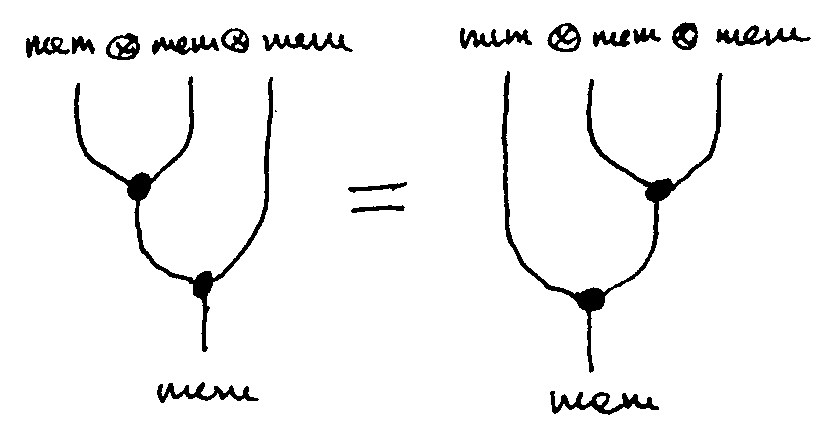
\includegraphics[scale=0.18]{draftfig/assoc}
\]

\[
  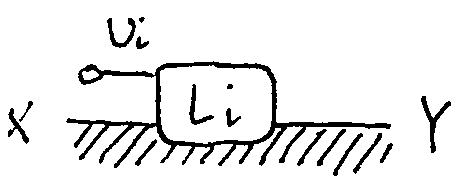
\includegraphics[scale=0.16]{draftfig/encap}
  \qquad\qquad
  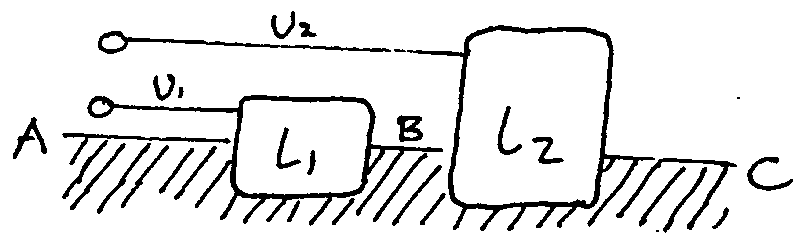
\includegraphics[scale=0.16]{draftfig/encap-comp}
\]

\[
  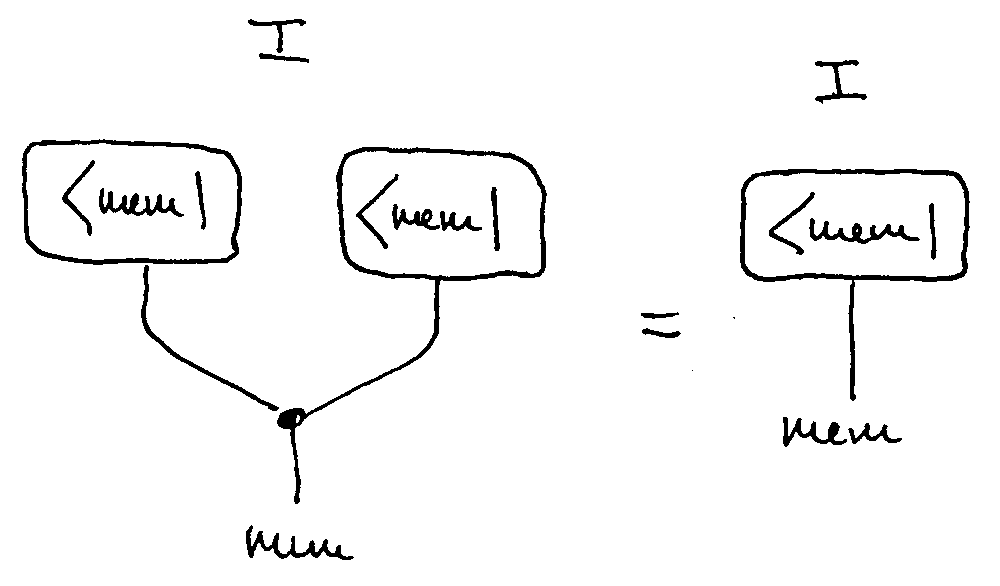
\includegraphics[scale=0.12]{draftfig/merge-caller}
  \qquad\qquad
  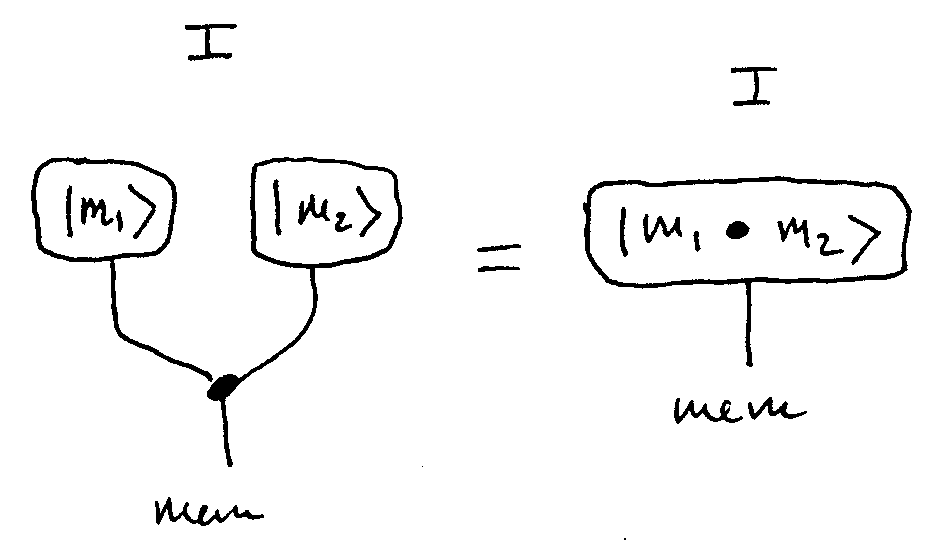
\includegraphics[scale=0.12]{draftfig/merge}
\]

%}}}

\section{Certified Abstraction Layers} \label{sec:cal} %{{{

This section will be dropped.

{
\color{gray}
A cleaner version of our OOPSLA story.
Here we must go from:
\begin{itemize}
  \item A fully abstract version where the layer interface
    has encapsulated abstract state,
    but does not change the memory at all
  \item A version where this is realized by an encapsulated
    memory component,
    which is added when the layer is invoked,
    and re-separated when it returns control to the client
    (refinement can act on that individual memory fragment).
  \item The concrete implementation version
    where the state is part of the global memory
    (refinement shown via
    simulation up to ${-} \bullet m \equiv {-}$).
\end{itemize}
}

We have shown in \ref{sec:base:abrel} that
abstraction relations are unwieldy,
especially when they are promoted to simulation conventions.

In general, the abstraction relations have the form
$R \subseteq K^\sharp \times (\kw{mem} \times K^\flat)$
so that the abstraction layers gradually refine
the concrete memory values and low-level abstract states
into high-level abstract states.
The abstraction relations are then promoted to simulation conventions
$\hat{R}: \mathcal{C}@(\kw{mem}\times K^\sharp)
\Leftrightarrow \mathcal{C}@(\kw{mem}\times K^\flat)$.
However, abstraction relations are not compatible with
vertical composition.
In other words, the following property does not hold
\[
   \hat{R \circ S} \sqsubseteq \hat{R}; \hat{S}
\]

The reason is that the abstraction relations
are playing two roles at the same time.
One is to refine the memory values to the abstract representations,
and the other is to embed the memory fragment
into the entire unified memory model.
Therefore, we seek to decouple the two tasks.
The $\ClightP$ language tackles the second task
and provides a more tractable $\kw{penv}$ interface
than the monolithic memory.
This leaves us the first task to solve.
With the help of state encapsulation,
the first task can be solved in a clean and elegant manner
as we will present.

\subsection{Layer Interfaces} %{{{

A layer interface with abstract states in $D$
can be defined using a transition system:
\[
  L : \mathbf{1} \twoheadrightarrow \mathcal{C}@D
\]
To interface with the client code,
we can hide the abstract state and lift the component to:
\[
  \Sigma := \kw{fbk}_D(\&L)@\kw{mem} : \mathbf{1} \rightarrow \mathcal{C}@\kw{mem}
\]
For example, we can hide the abstract state
from bounded queue and ring buffer interface in the example \ref{ex:rbspec}.
Note that the client may not modify their abstract states,
and may even not be aware of the existence of such states.
\[
  \Sigma_\kw{bq} := \kw{fbk}(\&L_\kw{bq}): \mathbf{1} \rightarrow \mathcal{C}@\kw{mem} \qquad
  \Sigma_\kw{rb} := \kw{fbk}(\&L_\kw{rb}): \mathbf{1} \rightarrow \mathcal{C}@\kw{mem}
\]

%}}}

\subsection{Layer Implementation}
\label{sec:cal:impl}

Given two transition systems manipulating states
at different abstraction levels
$L^\sharp: \mathbf{1} \twoheadrightarrow A@K^\sharp$
and
$L^\flat: \mathbf{1} \twoheadrightarrow A@K^\flat$,
the simulation between them is witnessed
by an abstraction relation $R \subseteq K^\sharp \times K^\flat$
such that
\[
  L^\sharp \le_{\kw{id} \twoheadrightarrow A@R} L^\flat
\]

Once the states are encapsulated,
the signatures of the two transition systems are identified.
As a consequence, the abstraction relation is concealed accordingly.
\[
  \kw{fbk}_{K^\sharp}(\& L^\sharp) \preceq \kw{fbk}_{K^\flat}(\& L^\flat)
\]
The secret is the simulation invariant.

The benefits of doing so:
\begin{itemize}
\item The self-simulation property for the client is no longer necessary.
  The client is ignorant of the representations.
  Decoupled the process of transforming the abstract state
  and assembling them into the memory.
  Again the secret is the simulation invariant.
\item The issues with composition of abstraction relations are solved
\end{itemize}

For the layer correctness,
we exploit the $\ClightP$ semantics as the implementation.
Then the correctness can be formulated as
\[
  \Sigma^\flat \vdash M : \Sigma^\sharp
  \Leftrightarrow
  \Sigma^\sharp \preceq \ClightP(M) \circ \Sigma^\flat
\]
The abstraction relation
$R \subseteq K^\sharp \times (\kw{penv} \times K^\flat)$
has once again been concealed.
Consequently, the vertical composition of abstraction layers
can be proved
by the monotonicity and associativity of layered composition
in a straightforward manner.
\[
  \begin{prooftree}
    \hypo{\Sigma^\flat \vdash M : \Sigma^\natural}
    \hypo{\Sigma^\natural \vdash N : \Sigma^\sharp}
    \infer2{\Sigma^\flat \vdash M, N : \Sigma^\sharp}
  \end{prooftree}
\]

Back to the bounded queue and ring buffer example,
we can prove the followings in the new framework
\[
  \Sigma_\kw{rb} \vdash M_\kw{bq} : \Sigma_\kw{bq}
  \qquad
  \varnothing \vdash M_\kw{rb} : \Sigma_\kw{rb}
\]
and then compose them together
\[
  \varnothing \vdash M_\kw{rb}, M_\kw{bq} : \Sigma_\kw{bq}
\]

{
\color{gray}
\subsection{Layer Implementation} %{{{

The correctness property $L^\flat \vdash M : L^\sharp$
must be established as a simulation of the form:
\[
  \kw{fbk}(\&L^\sharp)@\kw{mem}
  \le_\mathbb{R}
  \&\Clight(M) \circ \kw{fbk}(\&L^\flat)@\kw{mem}
  :
  \mathbf{1} \rightarrow \mathcal{C}@\kw{mem}
\]
Here the simulation convention $\mathbb{R}$
must exclude from the source memory
the region used in the target memory
to store the persistent state and stack frames used by $M$.
It must also ensure that
this region remains unchanged in the target memory
between successive activations of $M$.
However,
the exact representation used
to represent the hidden abstract state of $L^\sharp$
is itself hidden within the simulation.

\paragraph{Layer Correctness}

To prove a particular layer implementation correct,
we first focus on the way $M$ acts on its private fragment.
We give an abstraction relation
$R \subseteq D^\sharp \times (D^\flat \times \kw{mem})$
such that:
\begin{equation}
  L^\sharp
  \:\le_{\mathbf{1} \rightarrow \kw{id}@R}\:
  \Clight(M)@D^\flat \circ L^\flat@\kw{mem}
  \qquad \text{and} \qquad
  \intl{d}^\sharp \mathrel{R} \big( \intl{d}^{\,\flat}, \intl{m} \big)
  \,.
  \label{eqn:lc}
\end{equation}
Here $\intl{m}$ is the initial memory fragment for the module $M$,
derived from the definitions within $M$ itself.
Note that we can carry out this proof without regard for the context memory.
There are no particular conditions on $R$ other than
initial state being related.

\paragraph{Adding Context Memory}

By hiding internal state,
\autoref{eqn:lc} can be used to establish:
\begin{align*}
  \kw{fbk}_{D^\sharp}(\&L^\sharp) \le {} &
  \kw{fbk}_{D^\flat \times \kw{mem}} \big(
    \&(\Clight(M)@D^\flat \circ L^\flat@\kw{mem})
    \big) \\ \equiv {} &
  \kw{fbk}_\kw{mem}(\&\Clight(M)) \circ \kw{fbk}_{D^\flat}(\&L^\flat)
  : \mathbf{1} \rightarrow \mathcal{C}
  \,,
\end{align*}
however this does not take into account the context memory,
or the way in which the context memory and the memory used by $M$
are merged into the global memory
at the implementation level.
To achieve this we must use our memory separation primitive
and the frame rule for $\Clight$.
}

%Let me think about that but two things that come to mind:
%The first one is, for linking to work, you also need to do that for internal calls since the call from f to g will eventually become an internal call in [F + G] which will have to be matched with the cross-component interaction in [F] ⊕ [G].
%The second one is, think about the layer implementation case. We know that L : C@K ↠ C@K is refined by [[M]] : C@mem ↠ C@mem which operates in terms of a memory fragment that only contains the globals that implement abstract state K, and whatever stack blocks [[M]] allocates.
%Now the state for these transition systems is hidden so that we actually have a direct simulation between fbk(&L) : C → C and fbk(&L') : C → C. Both can then be lifted to fbk(&L)@mem, fbk(&L')@mem : C@mem → C@mem to be interfaced with context code. But note that in the execution of fbk(&L')@mem case there are now two different memory states involved: the context one which is left unchanged, and the 

%}}}

\subsection{Horizontal composition} %{{{

We first define the product.
\begin{definition}[Product] \label{def:prod}
  Given transition systems
\[
  L_1 = \langle S_1, {\rightarrow_1}, I_1, X_1, Y_1, T_1 \rangle
    : A \twoheadrightarrow B@K_1
  \quad \text{and} \quad
  L_2 = \langle S_2, {\rightarrow_2}, I_2, X_2, Y_2, T_2 \rangle
    : A \twoheadrightarrow B@K_2
\]
  we define
  $L_1 \cupdot L_2: A \twoheadrightarrow B@(K_1\times K_2)$
  as follows.
  \[
    S := (S_1 \times K_2) + (S_2 \times K_1)
  \]
  \[
    \begin{prooftree}
      \hypo{q@k_1 \mathrel{I_1} s_1}
      \infer1{q@(k_1, k_2) \mathrel{I} \iota_1(s_1@k_2)}
    \end{prooftree}
    \qquad
    \begin{prooftree}
      \hypo{s_1 \rightarrow_1 s'_1}
      \infer1{\iota_1(s_1@k_2) \rightarrow \iota_1(s'_1@k_2)}
    \end{prooftree}
    \qquad
    \begin{prooftree}
      \hypo{s_1 \mathrel{X_1} m}
      \infer1{\iota_1(s_1@k_2) \mathrel{X} m}
    \end{prooftree}
  \]
  \[
    \begin{prooftree}
      \hypo{n \mathrel{Y_1}^{s_1} s'_1}
      \infer1{n \mathrel{Y}^{s_1@k_2} \iota_1(s'_1@k_2)}
    \end{prooftree}
    \qquad
    \begin{prooftree}
      \hypo{s_1 \mathrel{F_1} r@k_1}
      \infer1{\iota_1(s_1@k_2) \mathrel{F} r@(k_1,k_2)}
    \end{prooftree}
  \]
  the symmetric cases are elided
\end{definition}

Then apply it to the components with encapsulated states.
\begin{definition}[Product] \label{def:sprod}
  Given two stateful components
$\Sigma_1 = (K_1 \mid L_1) : A \rightarrow B$ and
$\Sigma_2 = (K_2 \mid L_2) : A \rightarrow B$,
we define their composition
$\Sigma_1 \cup \Sigma_2 : A \rightarrow B$
in the following way:
\[
  \Sigma_1 \cup \Sigma_2 :=
    ( K_1 \times K_2 \mid L_1 \cupdot L_2 )
\]
\end{definition}

The horizontal composition can be proved
by the monotonicity and interchangeability.
\[
  \begin{prooftree}
    \hypo{\Sigma_1^\flat \vdash M : \Sigma_1^\sharp}
    \hypo{\Sigma_2^\flat \vdash N : \Sigma_2^\sharp}
    \infer2{\Sigma_1^\flat \cup \Sigma_2^\flat
      \vdash M, N : \Sigma_1^\sharp \cup \Sigma_2^\sharp}
  \end{prooftree}
\]

For example, this indicates that we can further
decompose the ring buffer layer into three layers,
and verify them independently.

%}}}

\subsection{Upcalls} %{{{

%}}}

%}}}

\section{Cut material to keep for now}

\begin{remark}[to incorporate or cut]
In particular,
in the absence of demonic nondeterminism,
CompCert's notion of \emph{forward simulation} is appropriate:
given two transition systems $L_1$ and $L_2$,
it suffices to exhibit a relation between their possible states
such that:
\begin{itemize}
  \item initial state of $L_1$ have related initial states in $L_2$;
  \item state transitions in $L_1$ have corresponding sequences of transitions
    from related states in $L_2$;
  \item related state which produce a final outcome in $L_1$
    have a corresponding final outcome in $L_2$.
\end{itemize}
To take into account event traces,
the simulation works under the assumption that
$L_1$ and $L_2$ are fed the same inputs by the environement,
and requires that they produce identical outputs.
The existence of a simulation relation satisfying these properties
shows that the behavior of $L_1$ is refined by that of $L_2$;
we say that $L_1$ is simulated by $L_2$ and write $L_1 \le L_2$.
\end{remark}

\begin{definition} [Simulation Convention Refinement] \label{def:scref}
  Given the stateful simulation conventions
  $\mathbf{R} : A^\sharp \leftrightarrow A^\flat$ and
  $\mathbf{S} : A^\sharp \leftrightarrow A^\flat$,
  the refinement between $\mathbf{R}$ and $\mathbf{S}$ is defined as:
  \[
    \mathbf{R} \sqsubseteq \mathbf{S} :\Leftrightarrow
    \mathbf{1} \preceq_{\mathbf{S} \twoheadrightarrow \mathbf{R}} \mathbf{1}
  \]
We write $\mathbf{R} \equiv \mathbf{S}$ when
$\mathbf{R} \sqsubseteq \mathbf{S}$ and
$\mathbf{S} \sqsubseteq \mathbf{R}$.
\end{definition}

The notion $\mathbf{1}$ represents the identify transition system.
Essentially, the refinement corresponds to the following indefinite condition:
\begin{align*}
  \forall w^R_1\ q^\sharp_1\ q^\flat_1.\ \intl{w^R} \mapsto w^R_1
  \Vdash q^\sharp_1 \mathrel{\mathbf{R}^\que} q^\flat_1 &\rightarrow
  \exists w^S_1.\ \intl{w^S} \mapsto w^S_1 
  \Vdash q^\sharp_1 \mathrel{\mathbf{S}^\que} q^\flat_1 \wedge\\
  \forall w^S_2\ r^\sharp_1\ r^\flat_1.\ w^S_1 \leadsto w^S_2
  \Vdash r^\sharp_1 \mathrel{\mathbf{S}^\ans} r^\flat_1 &\rightarrow
  \exists w^R_2.\ w^R_1 \leadsto w^R_2
  \Vdash r^\sharp_1 \mathrel{\mathbf{R}^\ans} r^\flat_1 \wedge\\
  \forall w^R_3\ q^\sharp_2\ q^\flat_2.\ w^R_2 \mapsto w^R_3
  \Vdash q^\sharp_2 \mathrel{\mathbf{R}^\que} q^\flat_2 &\rightarrow
  \exists w^S_3.\ w^S_2 \mapsto w^S_3
  \Vdash q^\sharp_3 \mathrel{\mathbf{S}^\que} q^\flat_3 \wedge\\
  \forall w^S_4\ r^\sharp_2\ r^\flat_2.\ w^S_3 \mapsto w^S_4
  \Vdash r^\sharp_2 \mathrel{\mathbf{S}^\ans} r^\flat_2 &\rightarrow
  \exists w^R_4.\ w^R_3 \mapsto w^R_4
  \Vdash r^\sharp_2 \mathrel{\mathbf{R}^\ans} r^\flat_2 \wedge\\[-1ex]
  &\:\:\vdots
\end{align*}

Similar to the refinement of the stateless simulation conventions,
a stateful simulation convention $\mathbf{S}$
is considered more general than $\mathbf{R}$
if the refinement $\mathbf{R} \sqsubseteq \mathbf{S}$ holds.
In particular, questions related by any worlds of $\mathbf{R}$
are also related under some worlds of $\mathbf{S}$;
when response is returned,
answers related at any successive worlds of $\mathbf{S}$
are also related under some successive worlds of $\mathbf{R}$.
However, because the questions and replies related
by a stateful simulation convention
are subject to the transition of its world,
the refinement unfolds indefinitely as the world evolves.

In general, in order to prove the stateful simulation between components
one has to design the simulation relation and invariant.
However, for proving simulation convention refinement,
there is not much to say about the states in the identity transition system.
So the simulation invariant is the key ingredient to prove such properties.


\begin{theorem}[Sequential rule of simulation convention] \label{thm:scseq}
  \[
    \begin{prooftree}
      \hypo{\mathbf{R'} \sqsubseteq \mathbf{R}}
      \hypo{L_1 \preceq_{\mathbf{R} \twoheadrightarrow \mathbf{S}} L_2}
      \hypo{\mathbf{S} \sqsubseteq \mathbf{S'}}
      \infer3{L_1 \preceq_{\mathbf{R'} \twoheadrightarrow \mathbf{S'}} L_2}
    \end{prooftree}
  \]
\end{theorem}

\section{ClightP}
\label{sec:clightp-1}


{
\color{gray}
[Note: this could be swapped with Section 3
because it showcases the use of persistent state,
but probably does not have much to gain
from the memory separation framework.]

Can we add a $\mathsf{private}$ keyword or storage class to Clight,
formulate a semantics and show a correctness proof
for erasure of the keyword?

Main challenge: how to define the semantics of the new keyword
in a way that's convenient.

We need a good name for this language.
For now I will use \ClightP{}.
}

Unlike the temporaries,
the module-local variables can also have type array or struct.
Therefore, we extend the type $\kw{val}$ with composite types to $\kw{cval}$
and define the $\kw{penv}$ as a map from identifiers to $\kw{cval}$.
Lifting the variables from memory to a separate environment
means that their address cannot be taken.
So we introduce accessors $\kw{lcval}$ to simulate left values,
which represent memory locations in $\Clight$,
so that the module-static variables can be evaluated to left values similarly
and updated accordingly.
Under this approach, struct assignment is not supported
because it is only possible to assign by value.
However, this enforces the program not to pass the address
of the private variables to other modules
so that undesired behaviors can be avoided.

\begin{gather*}
  cv \in \kw{cval} \mathrel{::=} \kw{Val}(v:\kw{val})
                     \mathrel{|} \kw{Arr}(sz:\mathbb{N},a:\mathbb{Z} \rightarrow \kw{cval})
  \\
  \kw{penv} \mathrel{::=} \kw{ident} \rightarrow \kw{cval}
  \\
  l \in \kw{lcval} \mathrel{::=} \kw{Lval}(i: \kw{ident})
                          \mathrel{|} \kw{Lloc}(l:\kw{lcval}, x:\mathbb{Z})
\end{gather*}

We reuse the $\Clight$ expressions,
and add the following expressions to access the private variables.
Similarly, we reuse the statements and small-step transitions
and add extra cases for updating the private states.
\begin{gather*}
  e \mathrel{::=} \cdots \mathrel{|} \kw{Epvar}(i:\kw{ident})
  \mathrel{|} \kw{Eaccess}(e:\kw{expr}, x: \kw{expr})
  \\[2ex]
  \kw{pread} \mathrel{:} \kw{penv} \rightarrow \kw{lcval} \rightarrow \kw{option}\ \kw{val}\\
  \kw{pwrite} \mathrel{:} \kw{penv} \rightarrow \kw{lcval} \rightarrow \kw{val} \rightarrow \kw{option}\ \kw{penv}
  \\[2ex]
  {\begin{prooftree}
    \hypo{\kw{pe}[i] = \lfloor \kw{Val}(v) \rfloor }
    \infer1{\kw{m},\kw{pe} \vdash \kw{Epvar}(i) \downarrow v}
  \end{prooftree}}
  \qquad
  {\begin{prooftree}
    \hypo{\kw{m}, \kw{pe} \vdash e \Downarrow loc}
    \hypo{\kw{m},\kw{pe} \vdash x \downarrow \kw{Vint}(i)}
    \hypo{\kw{pread}(\kw{pe}, \kw{Lloc}(loc, i)) = \lfloor \kw{Val}(v) \rfloor }
    \infer3{\kw{m},\kw{pe} \vdash \kw{Eaccess}(e, x) \downarrow v}
  \end{prooftree}}
  \\[2ex]
  {\begin{prooftree}
    \infer0{\kw{m},\kw{pe} \vdash \kw{Epvar}(i) \Downarrow \kw{Lval}(i)}
  \end{prooftree}}
  \qquad
  {\begin{prooftree}
    \hypo{\kw{m},\kw{pe} \vdash e \Downarrow loc}
    \hypo{\kw{m},\kw{pe} \vdash x \downarrow \kw{Vint}(i)}
    \infer2{\kw{m}, \kw{pe} \vdash \kw{Eaccess}(e, x) \Downarrow \kw{Lloc}(loc, i)}
  \end{prooftree}}
  \\[2ex]
  {\begin{prooftree}
    \hypo{\kw{m}, \kw{pe} \vdash a_1 \Downarrow loc}
    \hypo{\kw{m}, \kw{pe} \vdash a_2 \downarrow v}
    \hypo{\kw{pwrite}(pe, loc, v) = \lfloor pe' \rfloor }
    \infer3{(\kw{m}, \kw{pe}, \kw{Sassign}(a_1, a_2)) \rightarrow
      (\kw{m}, \kw{pe'}, \kw{Sskip})}
  \end{prooftree}}
\end{gather*}

A \ClightP{} program can be compiled to Clight
by erasing the \texttt{private} annotations
and turning privates variable into regular
global variables.
{
\color{gray}
Proving the correctness of this transformation
should not be too difficult.
We can just use a memory extension or injection.
The only new part is that we must express
the simulation convention for the underlying transition systems
in a way that relates the source private environment
to the target (public) memory state.
The twist here is that
the externally observable simulation convention
should just enforce the empty permissions in the source memory.
The relation between the private state and the target memory
should be existentially quantified.
But this means we need requirements on the initial target memory as well.
We will have to set up our extended notion of simulation
in a way that supports those things.
}

$\ClightP$ expressions are turned into $\Clight$ expressions
by replacing accesses to the private variables
with accesses to the corresponding memory locations.
\begin{gather*}
  \kw{transl\_expr}(\kw{Epvar}(i)) = \kw{Evar}(i)\\
  \kw{transl\_expr}(\kw{Eaccess}(e, \iota_2(i))) = \kw{Oadd}(\kw{transl\_expr(e)}, \kw{transl\_expr(i)})
\end{gather*}
The semantics of $\Clight$ is typed-directed
so the offset calculated by $\kw{Oadd}$
depends on the type of the array elements.
After the expressions are transated, the statements
are immediately valid $\Clight$ statements.

To establish the simulation between
the source $\ClightP$ program and the target $\Clight$ program,
we essentially transform the persistent environment into memory fragment,
and merge the fragment with the regular memory state.
We define a relation $\kw{pe} \rhd \kw{m}$
to denote that the the persistent environment $\kw{pe}$
can be concretized to the memory $\kw{m}$ under the global symbol table $\kw{se}$.
\[
  \begin{prooftree}
    \hypo{\forall i \mapsto cv \in \kw{pe}, \exists i \mapsto b \in se,
      (b,0) \leadsto_{\kw{m}} cv}
    \infer1{\kw{pe} \rhd \kw{m}}
  \end{prooftree}
\]
We define $(b, o) \leadsto_{\kw{m}} cv$ as follows:
\begin{gather*}
  {
  \begin{prooftree}
    \hypo{\kw{load}(\kw{m}, b, o) = \lfloor v \rfloor }
    \infer1{(b, o) \leadsto_{\kw{m}} \kw{Val}(v)}
  \end{prooftree}
  }
  \quad
  {
  \begin{prooftree}
    \hypo{\forall i, (b, o+\kw{offset}(a, i)) \leadsto_{\kw{m}} a[i]}
    \infer1{(b, o) \leadsto_{\kw{m}} \kw{Arr}(sz, a)}
  \end{prooftree}
  }
\end{gather*}
The auxiliary function $\kw{offset}$
calculates the offset based on the type information
which is elided for readability.

The other part of memory should remain the same.
We exploit the join operator defined in \ref{sec:sep}.

\section{Stashed examples}

\begin{example}[Layer specifications] \label{ex:rbspec} %{{{
We can formulate a specification for
the program component $\kw{rb.c}$ as follows.
The state of the ring buffer
is expressed as a tuple
$(f, c_1, c_2) \in S_\kw{rb} := \kw{val}^N \times \mathbb{N} \times \mathbb{N}$.
Operations do not otherwise access the memory,
so the specification will be of type
\[
  L_\kw{rb} : \mathbf{1} \twoheadrightarrow \mathcal{C}@S_\kw{rb}
  \,.
\]
To define it, we construct a simple transition system such that
all executions take the shape
\[
  q@(f, c_1, c_2) \:\mathrel{I}\: (v', f', c_1', c_2')
                  \:\mathrel{F}\: v'@(f', c_1', c_2')
  \,.
\]
The predicates $X$, $Y$ and $\rightarrow$ are empty.
As suggested above, $F$ is in essence the identity relation.
This leaves us to define $I$ which specifies the component's
actual behavior:
\[ \begin{array}{c@{\qquad}c}
 {\begin{prooftree}
    \hypo{i < N}
    \infer1{
      \kw{set}(i, v)@(f, c_1, c_2)
      \mathrel{I_\kw{rb}}
      (\kw{undef}, f[i := v], c_1, c_2)}
  \end{prooftree}}
  &
 {\begin{prooftree}
    \hypo{c_1' = (c_1 + 1) \mathbin{\mathrm{mod}} N}
    \infer1{
      \kw{inc1}@(f, c_1, c_2)
      \mathrel{I_\kw{rb}}
      (c_1, f, c_1', c_2)}
  \end{prooftree}}
  \vspace{1em}
  \\
 {\begin{prooftree}
    \hypo{i < N}
    \infer1{
      \kw{get}(i)@(f, c_1, c_2)
      \mathrel{I_\kw{rb}}
      (f_i, f, c_1, c_2)
    }
  \end{prooftree}}
  &
 {\begin{prooftree}
    \hypo{c_2' = (c_2 + 1) \mathbin{\mathrm{mod}} N}
    \infer1{
      \kw{inc1}@(f, c_1, c_2)
      \mathrel{I_\kw{rb}}
      (c_2, f, c_1, c_2')}
  \end{prooftree}}
\end{array} \]
We can then define
$L_\kw{rb} := \langle
  S_\kw{rb},\:
  \varnothing,\:
  I_\kw{rb},\:
  \varnothing,\:
  \varnothing,\:
  {=}
 \rangle$.

A similar approach can be use to define
$L_\kw{bq} : \mathbf{1} \twoheadrightarrow \mathcal{C}@S_\kw{bq}$,
where the states in $S_\kw{bq} := \kw{val}^*$
are simply lists enumerating the contents of the queue.
Here the operations will be specified as follows:
\[
  \begin{prooftree}
    \hypo{|\vec{q}| < N}
    \infer1{\kw{enq}(v)@\vec{q} \:\mathrel{I_\kw{bq}}\: (\kw{undef}, \vec{q}v)}
  \end{prooftree}
  \qquad\qquad
  \begin{prooftree}
    \hypo{\vec{q} = v\vec{p}}
    \infer1{\kw{deq}(\epsilon)@\vec{q} \:\mathrel{I_\kw{bq}}\: (v, \vec{p})}
  \end{prooftree}
\]
Again we can define $L_\kw{bq} := \langle
  S_\kw{bq},\:
  \varnothing,\:
  I_\kw{bq},\:
  \varnothing,\:
  \varnothing,\:
  {=}
\rangle$.
\end{example}
%}}}

\begin{example}[Interfacing $L_\kw{rb}$ with client code] \label{ex:context} %{{{
Building on Example~\ref{ex:rbspec},
consider the problem of interfacing
the client code in $\kw{bq.c}$ with the underlay interface $L_\kw{rb}$.
The types
\[
  L_\kw{rb} : \mathbf{1} \twoheadrightarrow \mathcal{C}@S_\kw{rb}
  \qquad
  \text{and}
  \qquad
  \Clight(\kw{bq.c}) : \mathcal{C}@\kw{mem} \twoheadrightarrow \mathcal{C}@\kw{mem}
\]
are not directly compatible,
given that $L_\kw{rb}$ manipulates a state of type $S_\kw{rb}$
and $\kw{rb.c}$ expects a memory state of type $\kw{mem}$.
The solution is to lift each one to ``pass through''
the state of the other:
\[
  \begin{tikzcd}[column sep=huge]
    \mathbf{1}@\kw{mem}
    \ar[r, "L_\kw{rb}@\kw{mem}"] &
    \mathcal{C}@S_\kw{rb}@\kw{mem} \cong
    \mathcal{C}@\kw{mem}@S_\kw{rb}
    \ar[r, "\Clight(\kw{bq.c})@S_\kw{rb}"] &
    \mathcal{C}@\kw{mem}@S_\kw{rb}
  \end{tikzcd}
\]
Implicitly taking into account the isomorphisms
\[
  \mathbf{1} \cong \mathbf{1}@\kw{mem}
  \qquad
  \text{and}
  \qquad
  \mathcal{C}@S_\kw{rb}@\kw{mem} \cong
  \mathcal{C}@\kw{mem}@S_\kw{rb} \cong
  \mathcal{C}@(S_\kw{rb} \times \kw{mem})
  \,,
\]
they can then be composed into
\begin{gather*}
  \Clight(\kw{bq.c})@S_\kw{rb} \odot
  L_\kw{rb}@\kw{mem} :
  \mathbf{1} \twoheadrightarrow \mathcal{C}@(S_\kw{rb} \times \kw{mem})
  \,.
\end{gather*}

To establish that this combination implements the overlay interface $L_\kw{bq}$,
we can lift the latter to:
\[
  L_\kw{bq}@\kw{mem} : \mathbf{1} \twoheadrightarrow
    \mathcal{C}@(S_\kw{bq} \times \kw{mem})
  \,.
\]
We will then need to define a simulation convention
explaining the relationship between
the states of type $S_\kw{bq}$ used by the specification and
the states of type $S_\kw{rb}$ used by the implementation.
\end{example}
%}}}

\section{Old intro}

\subsection{Verification Frameworks} \label{sec:intro:bigpict} %{{{

Building large-scale certified systems
requires the ability
to model and specify those systems compositionally,
so that verification can be carried out
on components of a manageable size.
In addition,
the verification of large heterogeneous systems---%
for example,
computer systems involving combinations of
hardware, software and network components---%
will require models versatile enough
to account for the large variety of
operational paradigms and interfaces involved.

Devising models that are up to the task is challenging,
but existing research has laid much of the necessary groundwork.
Denotational semantics and category theory
excel at describing and manipulating compositional structures.
They tend to focus on the externally observable behavior of components,
abstracting away any internal details which are irrelevant
to the ways in which components interact and combine.
In principle,
they could be used to achieve
large-scale compositionality for certified components.
However,
category theory and denotational semantics
have not seen widespread adoption
for certified software engineering.

By necessity,
many certified software projects use
specialized semantic models,
chosen first and foremost
to make verification tractable
in the context of a particular
programming language or verification target.
Any compositional structures they provide
are likewise fine-tuned to their particular setting.
In this context,
mandating the use of any one model
%in order to achieve interoperability between
%certified system components
is unrealistic.
Instead,
researchers should attempt to establish
a hierarchy of semantic models
with varying degrees of generality.
Simple models could be used
in specific contexts in order to facilitate verification.
At the same time,
the resulting specifications and proofs
could be embedded into more flexible models
where they could interface
with other components.

With that said,
the high level of abstraction and generality of
existing compositional semantics
is not the only thing
standing in the way of their use for verification.
As a general rule,
work of this kind has focused on characterizing exactly
the space of behaviors which can be defined in a particular language.
By contrast,
verification often operates in much more open-ended settings.
The focus is the relationship between specifications and implementations,
involving both abstraction and program refinement.
A better understanding of how these concepts fit into
the paradigm of compositional semantics
is therefore another important task
to make the construction of
large-scale, heterogeneous, certified systems
tractable.

%In this paradigm,
%suitable high-level models would need to account
%for specifications, refinement and abstraction,
%which have not been a traditional focus
%for denotational semantics
%but which are the bread and butter of
%many verification frameworks.
%Conversely,
%compositional structures
%used in low-level models to facilitate verification
%should ideally be designed in such a way that
%they can be preserved when embedded into richer settings.
%This would allow compositional reasoning
%to cut across components of different kinds,
%even when they were originally verified
%using different low-level frameworks.

%In what follows,
%we use this lens
%to examine recent work on
%the certified compiler CompCert.

%We present a formal account
%of both horizontal and vertical compositionality
%as well as the \emph{certified abstraction layer}
%techniques used to verify
%the operating system kernel CertiKOS.
%We identify \emph{double categories}
%as an account of structures found in CompCertO,
%an extension of CompCert
%which provides a compositional semantic preservation theorem.
%We outline a high-level account
%of this semantic model
%and show how these high-level structures
%can be used to facilitate
%an implementation of certified abstraction layers
%within the framework provided by CompCertO.

%}}}

% xx where do interaction trees fit in the picture

\subsection{CompCert} %{{{

Work on
the certified C compiler CompCert \cite{compcert}
illustrates many challenging aspects of compositional verification.
CompCert is a C compiler written in the Coq proof assistant
which comes with a formal, mechanized proof of correctness:
the semantics of the source and target languages
are described as labeled transition systems,
and a simulation proof
shows that the behavior of the compiled program
refines the behavior of the source program.

%The original correctness theorem of
Originally,
CompCert
only modeled the compilation of whole programs.
To overcome this limitation,
researchers first attempted to make
the transition system model used by CompCert
more compositional,
and to update the compiler's semantic preservation property
to operate at the level of individual translation units
\cite{compcompcert}.
Because
this came at a high cost in terms of proof effort,
subsequent work on verified separate compilation
turned instead to the development of compositional
\emph{proof techniques}
within the context of a closed, whole-program semantics
(\S\ref{sec:related:compcert}).
%Another successful approach
%was explored by the work
However,
the recent work on CompCertO \cite{compcerto}
revisits compositional semantic preservation,
addressing its challenges
by incorporating data refinement
as a first-class citizen.
The flexibility
gained by this approach
makes it possible %---as in CompCertM---%
to reuse much of CompCert's existing
correctness proofs,
and to address any difficulties in composition
using external reasoning.

The semantic model of CompCertO
remains fairly specialized:
its goal is to minimize any changes needed to CompCert,
to eliminate any unnecessary complexity,
and to enable compositionality
to the exact extent required
for compositional semantic preservation to work.
%In particular,
%the model does not account for
%encapsulated state;
%it describes the behavior of individual function calls,
%independently of any prior history,
%and expect any persistent state
%to be passed by the environment at entry
%alongside the names and parameters of the function to be invoked.
%
Yet
the directness of the approach
%in terms of the programme outlined in \S\ref{sec:intro:bigpict},
%CompCertO's approach also opens up the possibility
opens the door to
a compositional embedding
of CompCertO's semantics and proofs
into richer models.
In fact,
we will show that CompCertO's model
already exhibits a surprisingly rich compositional structure,
and that once this structure has been brought to light,
it can be extended to account for encapsulated state
using fairly general constructions.

%We will show that CompCertO's model
%can be equipped with the structure of
%a \emph{double category}.
%Based on this view
%of CompCertO's open semantics,
%we can further extend the framework
%to support state encapsulation.
%Moreover,
%once they are brought to light,
%we can give an account of
%these compositional structures
%in terms of simpler and more abstract models,
%such as Reddy's
%coherence space model of objects
%\cite{objsem}.
%
%The main difficulty encountered in this work
%is the difference in data representation
%in the semantics of source and target programs.
%In CompCert's closed semantics,
%these differences play no role in
%the externally observable behavior of programs.
%Consequently,
%simulation proofs can capture these differences
%in the simulation relations they use.
%Simulation relations are existentially quantified
%within proofs,
%and can remain hidden in correctness statements.
%By contrast,
%in the context of compositional semantics,
%cross-component interactions which occur
%within a linked program become observable,
%and these internal details can no longer be ignored.

%}}}

\subsection{Certified abstraction layers} %{{{

The divide between abstract semantic models
and concrete verification projects
also exists in the context of \emph{certified abstraction layers},
a technique which
allows a complex program to be verified in steps,
and which was used in the construction of
the certified operating system kernel CertiKOS
\cite{popl15,ccal}.

Under this approach,
the verification begins first with the lowest-level layer of code,
which other parts of the program rely on.
Once verified,
this code can be given a high-level specification,
which hides the implementation details
and makes it possible to reason about client code
in terms of an abstract view
of the lower layer's state.
This abstract state
can be accessed only by calling into
the layer's interface,
realizing a form of state encapsulation
and data abstraction.

To implement this methodology,
CertiKOS uses a modified version of CompCert
called CompCertX,
which parameterizes the compiler's semantics and correctness proof
with a layer interface.
This requirement [is a problem but now we have a general-purpose CompCertO].

%This approach was 
%
%There are limitations to the way this approach
%was implemented for the verification of CertiKOS.
%This work reused the CompCert semantics,
%by augmenting its memory model
%with a layer-dependent \emph{abstract state} component,
%making it possible to connect the code verification
%with the compiler's correctness proof.
%However,
%this means that the formulation of certified abstraction layers
%used in this context
%was intimately tied to CompCert-specific constructs.

In addition,
while this approach allows code
to be verified in a piecemeal manner,
and allows reasoning at an appropriate level of abstraction
for each layer,
the method is not fully compositional
in the sense that it relies on \emph{closed} semantics.
The behavior of a given abstraction layer
can only be characterized
once a specification for the lower layer it builds on has been given,
reducing the flexibility of the framework.
This also forces verification to proceed
in a linear way,
so that when two parts of the code
are independent,
one must nonetheless be verified
as a client to a layer which includes the other.

To address these limitations,
more abstract models have been proposed
for certified abstraction layers
\cite{rbgs-cal,popl22},
inspired by game semantics and
coherence space models of objects \cite{objsem}.
These models have not been used
in the context of practical verification tasks,
but shed light on the underlying structures
involved in this methodology.

Based on our framework,
we propose a formulation of certified abstraction layers
which incorporates the best of both worlds:
on one hand,
like the original formulation,
it is based on CompCertO semantics
and seamlessly integrates
with the compiler's correctness theorem;
on the other hand,
like more recent work,
the categorical structures underlying its construction
are made explicit,
facilitating a more compositional approach
to certified abstraction layers.
To illustrate these capabilities,
we demonstrate the use of this framework
by verifying a simple example
found in prior work.

%}}}

\begin{example}[Certified Abstraction Layers] \label{ex:overview:lint} %{{{

Software systems are often constructed in layers:
basic data structures and functionality
are implemented by low-level code.
We can then rely on this code
without concern its implementation details
or the data representation it uses.
Instead,
a programmer writing client code
will understand and reason about
this layer of code
in terms of a more abstract mental picture
of its operation.
For example,
when using the functions $\kw{enq}$ and $\kw{deq}$
shown in Fig.~\ref{fig:code},
we can think of the bounded queue they provide
as a simple sequence of elements,
and ignore the mechanics
of the ring buffer used to implement it.
\emph{Certified abstraction layers}
formalize this methodology within CompCert
and were used to verify the operating system kernel
CertiKOS \cite{popl15}.

Modeling layers required a modification of CompCert's semantics
to incorporate an \emph{underlay interface}
described using an \emph{abstract state}.
%to achieve a limited form of compositionality.
The closed semantics of CompCert can be described as
\[
  \chi : \top \twoheadrightarrow \mathcal{C} \mathbin@ \kw{mem}
  \: \vdash \:
  \kw{Clight}_\chi[M] : \top \twoheadrightarrow \mathbf{I}
  \,,
  \quad \text{ where }
  \top := \langle \varnothing, \varnothing \rangle
  \text{ and }
  \mathbf{I} := \langle \mathbbm1, \mathbbm1 \rangle
  \,.
\]
The transition system $\kw{Clight}_\chi[M]$
is invoked with a trivial question ${*} \in \mathbf{I}^\que$,
which initiates the execution of the $\kw{main}$ function of $M$.
When $M$ invokes an external function,
the behavior of that function is obtained from the parameter $\chi$.
In the CertiKOS proof,
abstraction layers are formalized by using
a variant CompCertX,
whose semantic model can be described as:
\[
  \forall D \in \mathbf{Set}
  \: \mathbin. \:
  L^\flat :
    \top \twoheadrightarrow
    \mathcal{C} \mathbin@ \kw{mem} \mathbin@ D
  \: \vdash \:
  \kw{Clight}_{L^\flat}[M] :
    \top \twoheadrightarrow
    \mathcal{C} \mathbin@ \kw{mem} \mathbin@ D
  \,.
\]
This allows the semantics of $M$ to be evaluated
in the context of the \emph{underlay} interface $L^\flat$,
whose primitives are described in terms of
an \emph{abstract state} memory component of type $D$.
A specification for the code in \autoref{fig:code}
may use an abstract state in $S_\kw{bq} := \kw{val}^*$.
The corresponding layer interface
$L_\kw{bq} : \top \twoheadrightarrow
 \mathcal{C} \mathbin@ \kw{mem} \mathbin@ S_\kw{bq}$
will then generate traces such as:
\[
  L_\kw{bq} \:\vDash\:
  \kw{enq}(v) \mathbin@ m \mathbin@ \vec{q}
  \:\rightarrowtail\:
  \kw{undef} \mathbin@ m \mathbin@ \vec{q}v
  \qquad%\qquad
  L_\kw{bq} \:\vDash\:
  \kw{deq}() \mathbin@ m \mathbin@ v\vec{q}
  \:\rightarrowtail\:
  v \mathbin@ m \mathbin@ \vec{q}
\]
We can then evaluate and reason about any client code
in terms of this abstract representation:
\[
  \kw{Clight}_{L_\kw{bq}} \big[\,
  \begin{minipage}{13em}
\begin{minted}{C}
void rot() { enq(deq()); }
\end{minted}
  \end{minipage} \,\big]
\:\vDash\:
%  \qquad
%  \Rightarrow
%  \qquad
  \kw{rot}() \mathbin@ m \mathbin@ v\vec{q}
  \:\rightarrowtail\:
  {*} \mathbin@ m \mathbin@ \vec{q}v
  \,.
\]

We will use certified abstraction layers
to illustrate the flexibility of CompCertO's approach
and as an example application for the techniques we introduce.
\end{example}
%}}}

\begin{example}[Layer Semantics] %{{{
As noted in Example~\ref{ex:overview:lint},
the CertiKOS verification effort
required the entire correctness proof of CompCert
to be modified to operate in terms of an underlay interface.
We can achieve a similar effect in CompCertO
without any modification to the compiler,
by defining
\[
  \kw{Clight}_{L^\flat}[M] :=
    (\kw{Clight}(M) \mathbin@ D^\flat) \odot L^\flat
  \,.
\]
We will see that CompCertO's open simulations
make it possible to formulate layer correctness
in a reasonably straightforward way as well.
\end{example}

%Using this construction,
%a C layer interface $L^\flat$ which uses abstract states in $D$
%can be modeled as a transition system of type
%$
%  L^\flat : \top \twoheadrightarrow \mathcal{C}_\kw{m}@D
%$,
%using questions and answers of the form:
%\begin{align*}
%  (\mathcal{C}_\kw{m}@D)^\que &:=
%    \{ f(\vec{v})@(m, d) \mid
%       f \in \kw{ident},
%       \vec{v} \in \kw{val}^*,
%       m \in \kw{mem},
%       d \in D \}
%  \\
%  (\mathcal{C}_\kw{m}@D)^\ans &:=
%    \{ v'@(m', d') \mid
%       v' \in \kw{val},
%       m' \in \kw{mem},
%       d' \in D \}
%\end{align*}
%This leaves the question of evaluating client code
%running on top of the underlay $L$.
%}}}

\begin{example}[Abstraction relations] \label{ex:overview:absrel} %{{{
In \S\ref{sec:overview:slift},
we noted that a layer specification
$L^\sharp :
 \top \twoheadrightarrow \mathcal{C} \mathbin@ \kw{mem} \mathbin@ D^\sharp$
and its implementation
$\kw{Clight}_{L^\flat}[M] :
 \top \twoheadrightarrow \mathcal{C}_\kw{m}@D^\flat$
%in terms of an underlay $L^\flat$
are not directly comparable, owing to their
use of different abstract states.
We now show how to construct,
using the techniques that we have introduced,
a simulation convention suitable for
stating the desired correctness property.

Note the decomposition
$\mathcal{C}_\kw{m}@D \cong \mathcal{C} \otimes [\kw{mem}] \otimes [D]$.
When a layer specification $L^\sharp$ is implemented,
part of its abstract state $D^\sharp$ is realized as concrete values
stored in the global memory,
and part of it reflects the abstract state of the underlay in $D^\flat$.
The details of this can be expressed using a relation
$R \subseteq (\kw{mem} \times D^\sharp) \times (\kw{mem} \times D^\flat)$,
allowing us to state the layer correctness property as
\[
  L^\flat \vdash_R M : L^\sharp \quad :\Leftrightarrow \quad
    L^\sharp \le_{\top \twoheadrightarrow \mathcal{C} \otimes [R]}
    \llbracket M \rrbracket_{L^\flat}
  \,.
\]
To ensure that this relation is compatible with client code,
we must require that
\[
  \forall C \mathbin.
    \kw{Clight}(C)@D^\sharp
    \le_{\mathcal{C} \otimes [R] \twoheadrightarrow \mathcal{C} \otimes [R]}
    \kw{Clight}(C)@D^\flat
  \,.
\]
%Now consider an assembly version
%$L^\sharp_\mathcal{A} :
% \top \twoheadrightarrow \mathcal{A} \otimes [\kw{mem}] \otimes [D^\sharp]$
%of the specification, such that
%\[
%  L^\sharp
%  \le_{\top \twoheadrightarrow \mathbb{C} \otimes D^\sharp}
%  L^\sharp_\mathcal{A}
%  \,.
%\]
\end{example}
%}}}

\end{document}
%%% Local Variables: 
%%% mode: LaTeX
%%% TeX-command-extra-options: "-shell-escape"
%%% End:
